% =============================================================================
% EpiForecast-MX — Avance 3: Modelo Baseline
% Tecnológico de Monterrey × Instituto Mexicano del Seguro Social (IMSS)
% Equipo 01 · Febrero 2026
% =============================================================================
\documentclass[11pt,a4paper]{article}

% --- Paquetes ----------------------------------------------------------------
\usepackage[utf8]{inputenc}
\usepackage[T1]{fontenc}
\usepackage[spanish,es-tabla]{babel}
\usepackage[margin=2.5cm]{geometry}
\usepackage{graphicx}
\usepackage{booktabs}
\usepackage{amsmath,amssymb}
\usepackage{hyperref}
\usepackage{xcolor}
\usepackage{float}
\usepackage{caption}
\usepackage{subcaption}
\usepackage{adjustbox}

% --- Captions grises y centrados ---------------------------------------------
\captionsetup{
    font={small, color=imss-gray},
    labelfont={bf, color=imss-gray},
    justification=centering,
    singlelinecheck=true,
}
\captionsetup[lstlisting]{
    font={small, color=imss-gray},
    labelfont={bf, color=imss-gray},
    justification=centering,
    singlelinecheck=true,
}
\usepackage{multirow}
\usepackage{tabularx}
\usepackage{array}
\usepackage{longtable}
\usepackage{enumitem}
\usepackage{fancyhdr}
\usepackage{listings}
\usepackage{natbib}
\usepackage{url}
\usepackage{parskip}
\usepackage{titlesec}
\usepackage{pdfpages}
\usepackage{wrapfig}

% --- Colores IMSS institucionales --------------------------------------------
\definecolor{imss-burgundy}{HTML}{9B2242}
\definecolor{imss-teal}{HTML}{00524E}
\definecolor{imss-gold}{HTML}{B58500}
\definecolor{imss-black}{HTML}{231F20}
\definecolor{imss-gray}{HTML}{97999B}
\definecolor{imss-dk-burgundy}{HTML}{6F1D46}
\definecolor{imss-dk-teal}{HTML}{173F35}

% --- Configuración de hyperref -----------------------------------------------
\hypersetup{
    colorlinks=true,
    linkcolor=imss-teal,
    citecolor=imss-burgundy,
    urlcolor=imss-teal,
    bookmarksopen=true,
    pdftitle={EpiForecast-MX — Avance 3: Modelo Baseline},
    pdfauthor={Equipo 01 — Tecnológico de Monterrey},
}

% --- Configuración de listings (para bloques Tableau) ------------------------
\lstset{
    basicstyle=\small\ttfamily,
    backgroundcolor=\color{gray!8},
    frame=single,
    rulecolor=\color{imss-gray},
    breaklines=true,
    numbers=none,
    xleftmargin=1em,
    framexleftmargin=0.5em,
    captionpos=b,
}

% --- Encabezado y pie de página ----------------------------------------------
\pagestyle{fancy}
\fancyhf{}
\fancyhead[L]{\small\textcolor{imss-gray}{EpiForecast-MX — Avance 3}}
\fancyhead[R]{\small\textcolor{imss-gray}{Equipo 01 · Tec de Monterrey × IMSS}}
\fancyfoot[C]{\thepage}
\renewcommand{\headrulewidth}{0.4pt}
\renewcommand{\footrulewidth}{0pt}

% --- Ajuste de secciones -----------------------------------------------------
\titleformat{\section}{\Large\bfseries\color{imss-burgundy}}{\thesection}{1em}{}
\titleformat{\subsection}{\large\bfseries\color{imss-teal}}{\thesubsection}{1em}{}
\titleformat{\subsubsection}{\normalsize\bfseries\color{imss-dk-teal}}{\thesubsubsection}{1em}{}

% --- Nuevos comandos ---------------------------------------------------------
\newcommand{\padF}{\textbf{Depresión (F32)}}
\newcommand{\padG}{\textbf{Parkinson (G20)}}
\newcommand{\padA}{\textbf{Alzheimer (G30)}}

% =============================================================================
%  PORTADA
% =============================================================================
\begin{document}
\thispagestyle{empty}

\begin{center}

\vspace*{0.5cm}

% --- Logos -------------------------------------------------------------------
\begin{minipage}{0.35\textwidth}
    \centering
    
\includegraphics[height=2.5cm]{logo_tec.png}
\end{minipage}
\hfill
\begin{minipage}{0.35\textwidth}
    \centering
    
\includegraphics[height=2.5cm]{logo_imss.png}
\end{minipage}

\vspace{1.5cm}

{\LARGE\bfseries\textcolor{imss-burgundy}{EpiForecast-MX}}\\[0.4cm]
{\Large\bfseries Avance 3: Modelo Baseline}\\[0.3cm]
{\large \textbf{``Generalización de modelos nacionales de pronóstico epidemiológico hacia un enfoque modular con desagregación por sexo y entidad federativa en México''}}

\vspace{0.6cm}

{\large\textcolor{imss-burgundy}{Depresión (F32)} $\cdot$
\textcolor{imss-teal}{Parkinson (G20)} $\cdot$
\textcolor{imss-gold}{Alzheimer (G30)}}

\vspace{1.0cm}

\resizebox{\textwidth}{!}{%
\begin{tabular}{l l l}
\toprule
\textbf{Rol} & \textbf{Nombre} & \textbf{Institución} \\
\midrule
Estudiante — Desarrollo & Javier Augusto Rebull Saucedo & Tec de Monterrey / Santander US \\
Estudiante — Desarrollo & Juan Carlos Pérez Nava & Tec de Monterrey / IMSS \\
Estudiante — Desarrollo & Luis Gerardo Sánchez Salazar & Tec de Monterrey / Tesla \\
\addlinespace
Asesora Académica & Dra.\ Grettel Barceló Alonso & Tecnológico de Monterrey \\
Sponsor / Líder de Proyecto & Dra.\ Ruth Pérez & IMSS \\
Investigadora en Psiquiatría & Dra.\ Lina Díaz Castro & IMSS \\
\bottomrule
\end{tabular}%
}

\vspace{0.8cm}

{\large TC5035 — Proyecto Integrador\\
Módulo 3: Ingeniería y Evaluación de Modelos\\[0.2cm]
Maestría en Inteligencia Artificial Aplicada\\
Tecnológico de Monterrey}

\vspace{0.5cm}

{\large\bfseries Semana 05 · Febrero 2026}

\vspace{1.0cm}

% --- Enlaces oficiales -------------------------------------------------------
\begin{flushleft}
\small
\textcolor{imss-teal}{\textbf{Dashboard interactivo:}}\\
\url{https://proyectointegrador.org/epidashboard}\\[0.25cm]
\textcolor{imss-teal}{\textbf{Sitio oficial del proyecto:}}\\
\url{https://proyectointegrador.org}\\[0.25cm]
\textcolor{imss-teal}{\textbf{PDF Ejecutivo y Notebook completo:}}\\
\url{https://drive.google.com/drive/folders/1LRi0WzthWZgz2PaD7cno3xAxaPbRNpaG?usp=sharing}\\[0.25cm]
\textcolor{imss-teal}{\textbf{Repositorio oficial GitHub:}}\\
\url{https://github.com/IntegradorIMSS2026Team01/EpiForecast-MX}
\end{flushleft}

\end{center}

\newpage

% =============================================================================
%  RESUMEN
% =============================================================================
\section*{Resumen}
\addcontentsline{toc}{section}{Resumen}

El presente documento describe el desarrollo y evaluación de 297 modelos baseline de pronóstico epidemiológico para tres padecimientos neurológicos y de salud mental en México: Depresión (F32), Parkinson (G20) y Alzheimer (G30). Los modelos se construyeron utilizando el algoritmo Prophet \citep{taylor2018forecasting} y se evaluaron mediante validación cruzada temporal con cuatro métricas complementarias: MAPE, RMSE, MAE y MDAPE.

A nivel nacional, el modelo de Depresión alcanzó un MAPE de 14.60\% en validación cruzada, mientras que Parkinson y Alzheimer registraron 27.76\% y 28.30\%, respectivamente. El análisis por sexo reveló que los modelos masculinos presentan menor error en Depresión (13.80\% vs.\ 15.21\%) y Parkinson (28.04\% vs.\ 30.64\%), mientras que en Alzheimer las mujeres muestran mejor predecibilidad (31.18\% vs.\ 34.03\%). A nivel estatal, la mediana del MAPE fue de 37.79\% para Depresión, 65.62\% para Parkinson y 47.48\% para Alzheimer, con una dispersión significativa entre entidades federativas. Los mejores desempeños estatales correspondieron a Ciudad de México para Depresión (MAPE 4.79\%), Jalisco para Parkinson (36.04\%) y San Luis Potosí para Alzheimer (38.69\%). Se identificaron un total de 143 outliers en Depresión, 36 en Parkinson y 0 en Alzheimer.

Estos resultados establecen una línea base cuantitativa contra la cual se compararán los modelos optimizados del Avance~4.

\textbf{Palabras clave:} pronóstico epidemiológico, series de tiempo, Prophet, Depresión, Parkinson, Alzheimer, IMSS, México.

\newpage
\tableofcontents
\newpage

% =============================================================================
%  1. INTRODUCCIÓN Y CONTEXTO
% =============================================================================
\section{Introducción y Contexto}\label{sec:intro}

El pronóstico epidemiológico constituye una herramienta fundamental para la planificación y asignación de recursos en sistemas de salud pública. En el contexto del Instituto Mexicano del Seguro Social (IMSS), la capacidad de anticipar la incidencia de padecimientos neurológicos y de salud mental permitiría una gestión más eficiente de consultas, tratamientos y personal especializado.

El proyecto EpiForecast-MX aborda este desafío para tres padecimientos con características epidemiológicas distintas, codificados según la Clasificación Internacional de Enfermedades (CIE-10): Depresión (F32), Parkinson (G20) y Alzheimer (G30). Estos padecimientos fueron seleccionados en conjunto con las stakeholders del IMSS —la Dra.\ Ruth Pérez y la Dra.\ Lina Díaz Castro— por su relevancia clínica y su potencial impacto en la planificación operativa.

El presente avance tiene como objetivo construir un modelo de referencia (\emph{baseline}) para cada padecimiento que permita: (a) evaluar la viabilidad del pronóstico epidemiológico automatizado, (b) establecer un piso de desempeño contra el cual se compararán modelos optimizados en el Avance~4, (c) gestionar expectativas con los stakeholders del IMSS y (d) validar el pipeline de datos SINAVE--INEGI para las tres enfermedades.

Los datos provienen de los boletines epidemiológicos del Sistema Nacional de Vigilancia Epidemiológica (SINAVE), complementados con información demográfica del Instituto Nacional de Estadística y Geografía (INEGI). Las series temporales abarcan el período 2012--2025 con resolución semanal e incluyen la desagregación por entidad federativa y sexo.

% =============================================================================
%  2. METODOLOGÍA
% =============================================================================
\section{Metodología}\label{sec:metodo}

\subsection{Selección del Algoritmo: Prophet}\label{sec:justificacion-prophet}

La selección de Prophet \citep{taylor2018forecasting} como algoritmo baseline se fundamenta en los criterios del marco metodológico CRISP-ML(Q) \citep{studer2021crisp}:

\begin{itemize}[nosep]
    \item \textbf{Tipo de datos:} Series de tiempo semanales con estacionalidad anual y tendencia. Prophet está diseñado específicamente para este tipo de patrón temporal.
    \item \textbf{Robustez:} Maneja valores faltantes, outliers y \emph{changepoints} de forma nativa, aspecto crítico dado el efecto disruptivo del COVID-19 en los tres padecimientos.
    \item \textbf{Escalabilidad:} Pipeline parametrizable que ejecuta modelos idénticos por padecimiento, entidad y sexo sin cambio de arquitectura.
    \item \textbf{Interpretabilidad:} Descompone la serie en tendencia y estacionalidad, facilitando la comunicación con los stakeholders clínicos del IMSS.
    \item \textbf{Intervalos de predicción:} Genera bandas de incertidumbre nativamente, requisito fundamental para planificación en salud pública.
    \item \textbf{Evidencia previa:} La Fase~I del proyecto demostró que modelos ML recursivos (XGBoost, Random Forest) presentan acumulación progresiva de error en horizontes largos ($52+$ semanas).
\end{itemize}

\subsection{Descarte de Modelos Alternativos}\label{sec:descarte}

Se evaluaron y descartaron las siguientes alternativas:

\begin{table}[H]
\centering
\caption{Modelos descartados y razones de exclusión.}
\label{tab:descarte}
\begin{tabularx}{\textwidth}{@{}l X@{}}
\toprule
\textbf{Modelo} & \textbf{Razón de descarte} \\
\midrule
XGBoost / RF recursivo & La Dra.\ Grettel identificó \emph{data leakage} en la implementación de la Fase~I (reunión 12-feb-2026). La predicción recursiva multi-paso acumula error en horizontes de 84~semanas. \\
\addlinespace
ARIMA / SARIMA & Requieren estacionariedad estricta y especificación manual de órdenes. No manejan los \emph{changepoints} por COVID-19 de forma nativa. \\
\addlinespace
Modelo naïve & No captura la estacionalidad anual documentada en los tres padecimientos neurológicos y de salud mental. \\
\bottomrule
\end{tabularx}
\end{table}

\subsection{Estructura de Modelado}\label{sec:estructura}

Para cada uno de los tres padecimientos se construyeron modelos en cuatro niveles de granularidad:

\begin{table}[H]
\centering
\caption{Niveles de granularidad por padecimiento.}
\label{tab:niveles}
\begin{tabular}{@{}l c l@{}}
\toprule
\textbf{Nivel} & \textbf{Modelos} & \textbf{Propósito} \\
\midrule
Nacional & 1 & Visión macro del comportamiento epidemiológico \\
Nacional $\times$ Sexo & 2 & Identificar diferencias de género en la incidencia \\
Por Entidad Federativa & 32 & Pronóstico estatal para asignación de recursos \\
Entidad $\times$ Sexo & 64 & Máxima granularidad para planificación operativa \\
\addlinespace
\textbf{Total por padecimiento} & \textbf{99} & \\
\bottomrule
\end{tabular}
\end{table}

De esta forma, se entrenaron y evaluaron $3 \times 99 = 297$ modelos baseline en total.

\subsection{Métricas de Desempeño}\label{sec:metricas}

Se seleccionaron cuatro métricas complementarias que permiten comparar entre padecimientos con volúmenes de incidencia muy distintos (Depresión $\gg$ Parkinson $>$ Alzheimer) y que resultan interpretables para stakeholders no técnicos:

\begin{align}
\text{MAPE} &= \frac{100}{n}\sum_{i=1}^{n}\frac{|y_i - \hat{y}_i|}{|y_i|} \label{eq:mape} \\[6pt]
\text{RMSE} &= \sqrt{\frac{1}{n}\sum_{i=1}^{n}(y_i - \hat{y}_i)^2} \label{eq:rmse} \\[6pt]
\text{MAE} &= \frac{1}{n}\sum_{i=1}^{n}|y_i - \hat{y}_i| \label{eq:mae} \\[6pt]
\text{MDAPE} &= \text{mediana}\left(\frac{|y_i - \hat{y}_i|}{|y_i|}\right) \label{eq:mdape}
\end{align}

El MAPE (Ecuación~\ref{eq:mape}) constituye la métrica principal por su comparabilidad entre padecimientos y entidades. El RMSE (Ecuación~\ref{eq:rmse}) penaliza errores extremos que afectan la asignación de recursos. El MAE (Ecuación~\ref{eq:mae}) es directamente interpretable como diferencia promedio en casos. El MDAPE (Ecuación~\ref{eq:mdape}) complementa al MAPE con robustez ante outliers \citep{hyndman2006another}. Se excluyen observaciones con $y_i = 0$ del cálculo de MAPE y MDAPE, conforme a la advertencia de la Dra.\ Grettel sobre entidades con bajo reporte.

\subsection{Validación Cruzada Temporal}\label{sec:cv}

La evaluación se realizó mediante validación cruzada temporal \citep{bergmeir2012use} con los siguientes parámetros, establecidos por recomendación de la Dra.\ Grettel:

\begin{itemize}[nosep]
    \item \textbf{initial:} 730 días ($\approx$2 años de entrenamiento mínimo).
    \item \textbf{period:} 56 días ($\approx$8 semanas entre cortes de validación).
    \item \textbf{horizon:} 168 días ($\approx$24 semanas de horizonte evaluado).
\end{itemize}

Esta configuración asegura que el modelo es evaluado de forma realista con ventanas deslizantes que simulan el escenario operativo de pronóstico, respetando la naturaleza temporal de los datos.

\subsection{Detección de Outliers}\label{sec:outliers}

Se implementó el método del rango intercuartílico (IQR) \citep{tukey1977exploratory} con factor $k=1.5$ para la identificación de valores atípicos en cada serie. Un dato $y_i$ se clasifica como outlier si:
\begin{equation}
y_i < Q_1 - 1.5 \cdot \text{IQR} \quad \text{ó} \quad y_i > Q_3 + 1.5 \cdot \text{IQR}
\label{eq:iqr}
\end{equation}
donde $Q_1$ y $Q_3$ son el primer y tercer cuartil, respectivamente, e $\text{IQR} = Q_3 - Q_1$.

% =============================================================================
%  3. RESULTADOS POR PADECIMIENTO
% =============================================================================
\section{Resultados por Padecimiento}\label{sec:resultados}

Esta sección presenta los resultados del modelo baseline a nivel nacional para cada uno de los tres padecimientos. La Tabla~\ref{tab:metricas-nacionales} consolida las métricas de los nueve modelos nacionales (tres padecimientos $\times$ tres niveles).

\begin{table}[H]
\centering
\caption{Métricas de desempeño de los modelos nacionales (validación cruzada temporal).}
\label{tab:metricas-nacionales}
\resizebox{\textwidth}{!}{%
\begin{tabular}{@{}l l r r r r r r r r r@{}}
\toprule
\textbf{Padecimiento} & \textbf{Nivel} & \textbf{MAPE (\%)} & \textbf{RMSE} & \textbf{MAE} & \textbf{MDAPE} & \textbf{MAPE\textsubscript{train} (\%)} & \textbf{RMSE\textsubscript{train}} & \textbf{MAE\textsubscript{train}} & \textbf{Brecha (pp)} & \textbf{Outliers} \\
\midrule
Depresión & Nacional       & 14.60 & 396.68 & 270.89 & 0.088 & 9.37 & 275.28 & 165.12 & 5.22 & 6 \\
Depresión & Hombres        & 13.80 & 99.83  & 69.35  & 0.091 & 9.58 & 74.91  & 44.42  & 4.22 & 5 \\
Depresión & Mujeres        & 15.21 & 301.63 & 206.45 & 0.088 & 10.06 & 209.47 & 129.89 & 5.15 & 5 \\
\addlinespace
Parkinson & Nacional       & 27.76 & 39.07  & 28.82  & 0.149 & 20.37 & 26.46  & 20.07  & 7.39 & 24 \\
Parkinson & Hombres        & 28.04 & 20.84  & 15.89  & 0.159 & 22.78 & 15.30  & 11.79  & 5.27 & 26 \\
Parkinson & Mujeres        & 30.64 & 19.48  & 14.45  & 0.162 & 23.31 & 14.01  & 10.85  & 7.34 & 18 \\
\addlinespace
Alzheimer & Nacional       & 28.30 & 11.55  & 8.64   & 0.164 & 23.41 & 8.77   & 6.76   & 4.90 & 5 \\
Alzheimer & Hombres        & 34.03 & 5.45   & 4.19   & 0.200 & 28.85 & 4.38   & 3.49   & 5.18 & 2 \\
Alzheimer & Mujeres        & 31.18 & 7.05   & 5.41   & 0.186 & 27.19 & 5.65   & 4.39   & 3.99 & 4 \\
\bottomrule
\end{tabular}%
}
\end{table}

\subsection{Depresión (F32)}\label{sec:depresion}

La Depresión constituye el padecimiento con mayor volumen de incidencia reportada en SINAVE. El modelo nacional alcanzó un MAPE de 14.60\% en validación cruzada, clasificándose como \emph{Excelente} según los umbrales definidos en la Sección~\ref{sec:desempeno}. La brecha entre el error de entrenamiento (9.37\%) y el de validación (14.60\%) es de 5.22 puntos porcentuales, indicando un nivel moderado de sobreajuste consistente con la complejidad de la serie. Se detectaron 6~outliers a nivel nacional.

El análisis por sexo reveló que el modelo masculino presenta menor error (MAPE 13.80\%) frente al femenino (15.21\%), con una diferencia de 1.41 puntos porcentuales. Esta diferencia puede atribuirse a la mayor variabilidad en los patrones de consulta femenina, dato relevante para el prorrateo proporcional solicitado por las stakeholders del IMSS.

\begin{figure}[H]
\centering
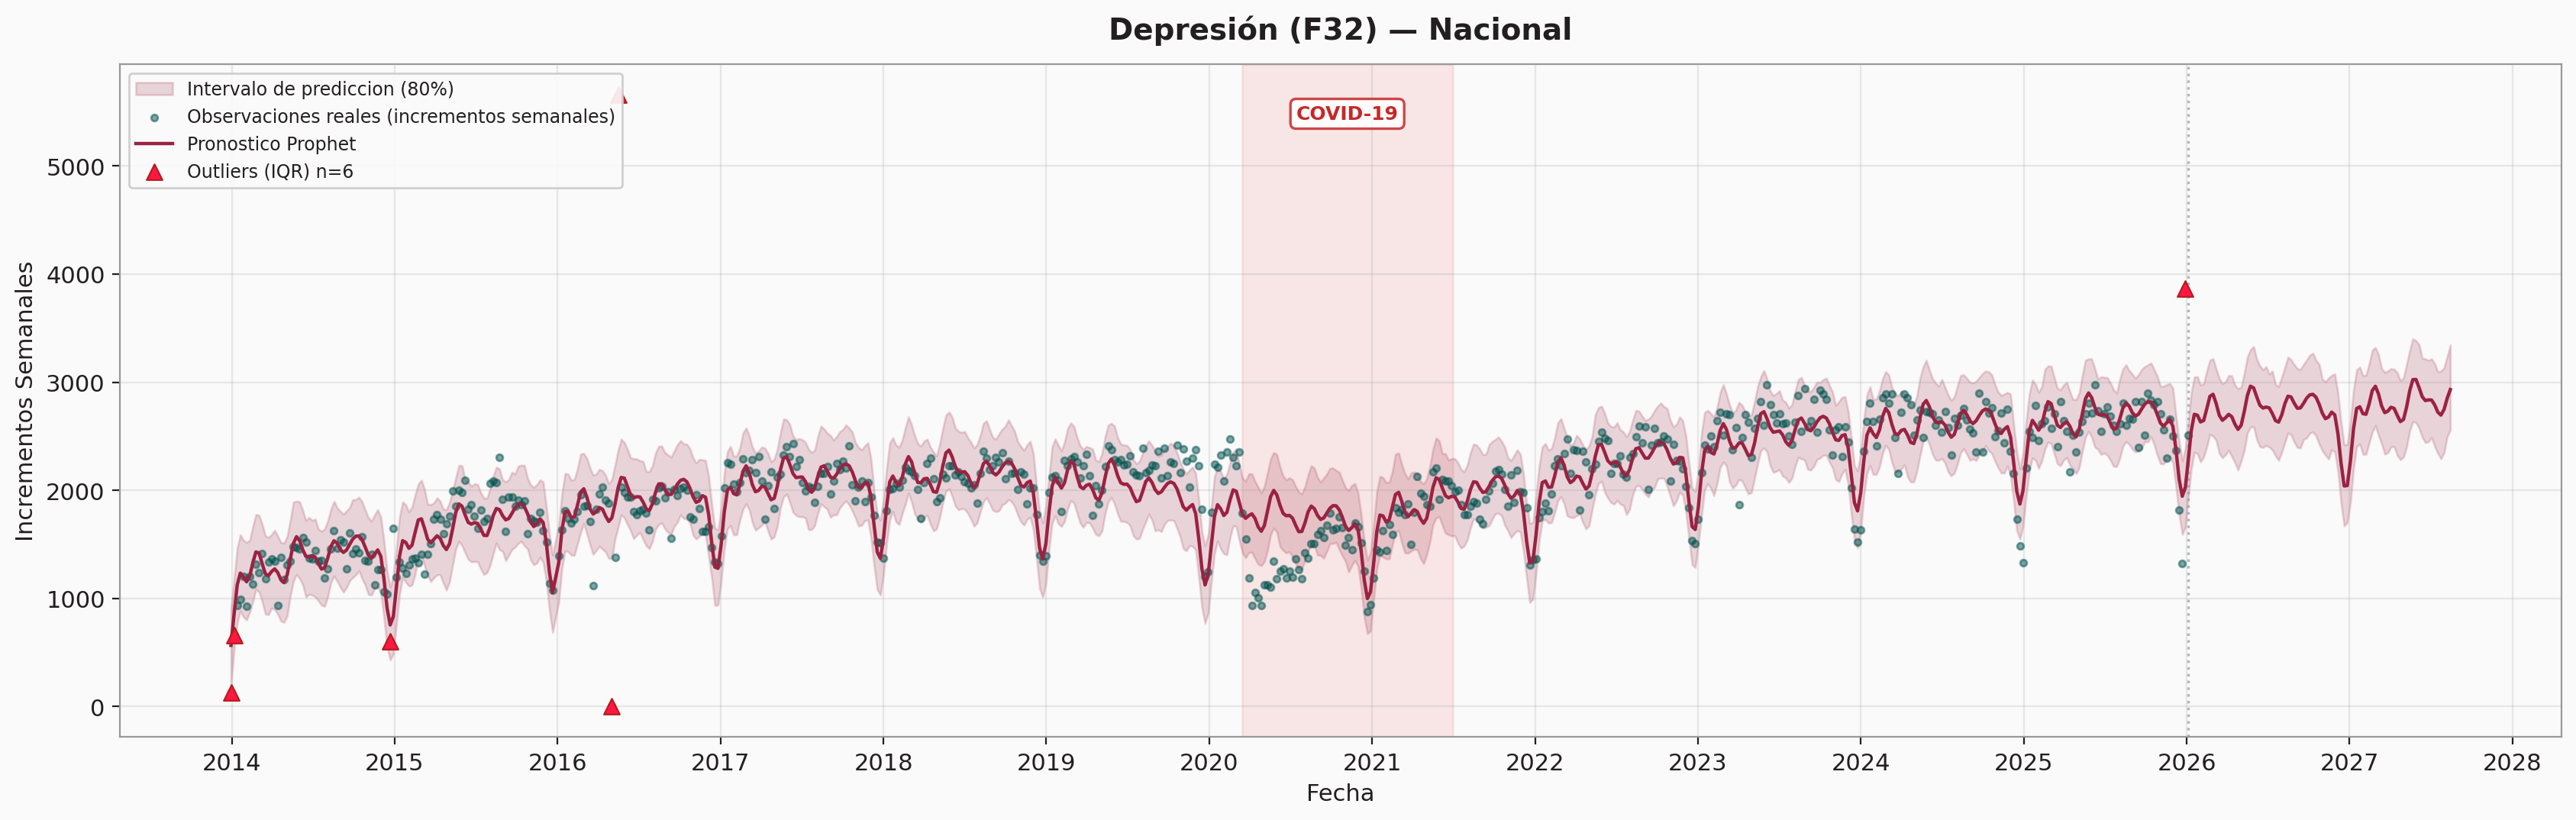
\includegraphics[width=\textwidth]{fig_01_F32_Depresion_nacional_pronostico.png}
\caption{Pronóstico nacional — Depresión (F32). Los puntos verdes representan observaciones reales, la línea roja el pronóstico Prophet, la banda sombreada el intervalo de predicción al 80\%, la franja roja el período COVID-19 y los triángulos rojos los valores atípicos detectados por IQR.}
\label{fig:f32-pronostico}
\end{figure}

\begin{figure}[H]
\centering
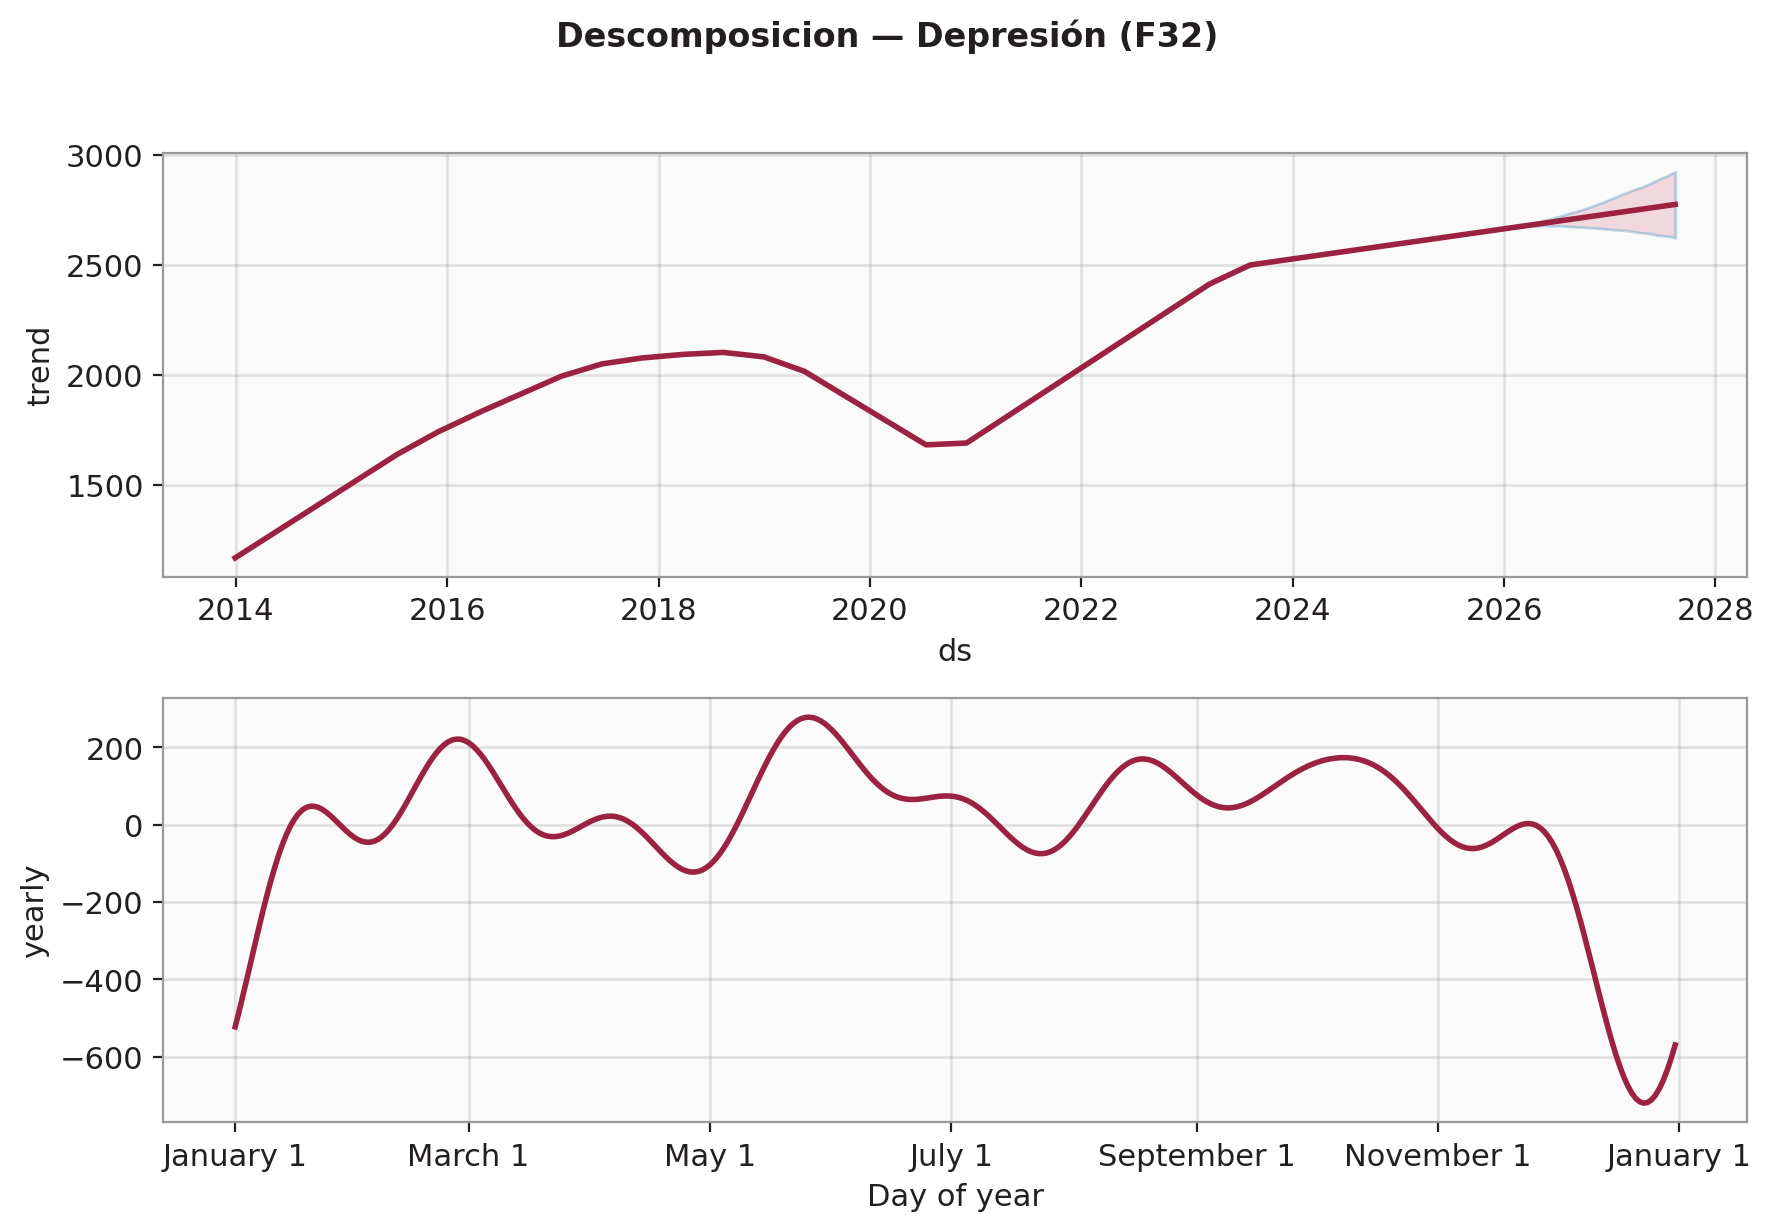
\includegraphics[width=\textwidth]{fig_02_F32_Depresion_nacional_componentes.png}
\caption{Descomposición en componentes — Depresión (F32). Panel superior: tendencia a largo plazo. Panel inferior: estacionalidad anual.}
\label{fig:f32-componentes}
\end{figure}

\begin{figure}[H]
\centering
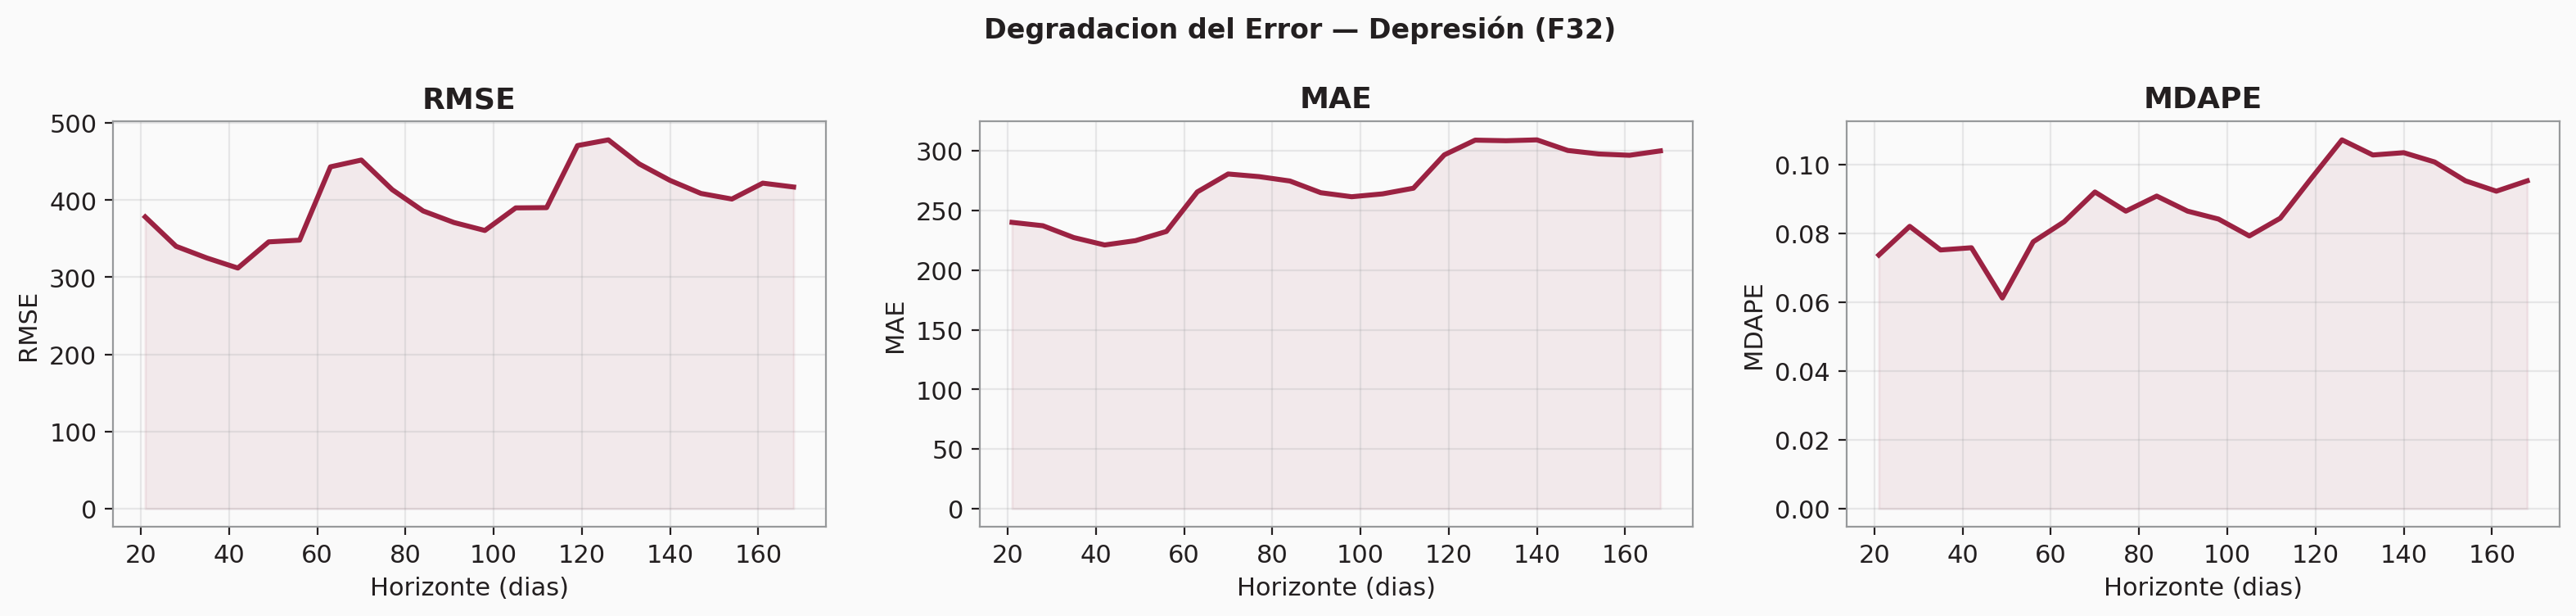
\includegraphics[width=\textwidth]{fig_03_F32_Depresion_nacional_cv_horizonte.png}
\caption{Degradación del error por horizonte de pronóstico — Depresión (F32). Se observa cómo el error de predicción aumenta conforme se extiende el horizonte temporal.}
\label{fig:f32-cv}
\end{figure}

\subsection{Parkinson (G20)}\label{sec:parkinson}

El modelo nacional de Parkinson registró un MAPE de 27.76\%, clasificándose como \emph{Aceptable}. Este padecimiento presenta la mayor brecha entre entrenamiento y validación (7.39~pp), sugiriendo mayor dificultad para generalizar, probablemente asociada al bajo volumen de incidencia y la irregularidad del reporte estatal. Se detectaron 24~outliers a nivel nacional.

La diferencia por sexo es de 2.60 puntos porcentuales (28.04\% en hombres vs.\ 30.64\% en mujeres), siendo nuevamente los modelos masculinos los de menor error.

\begin{figure}[H]
\centering
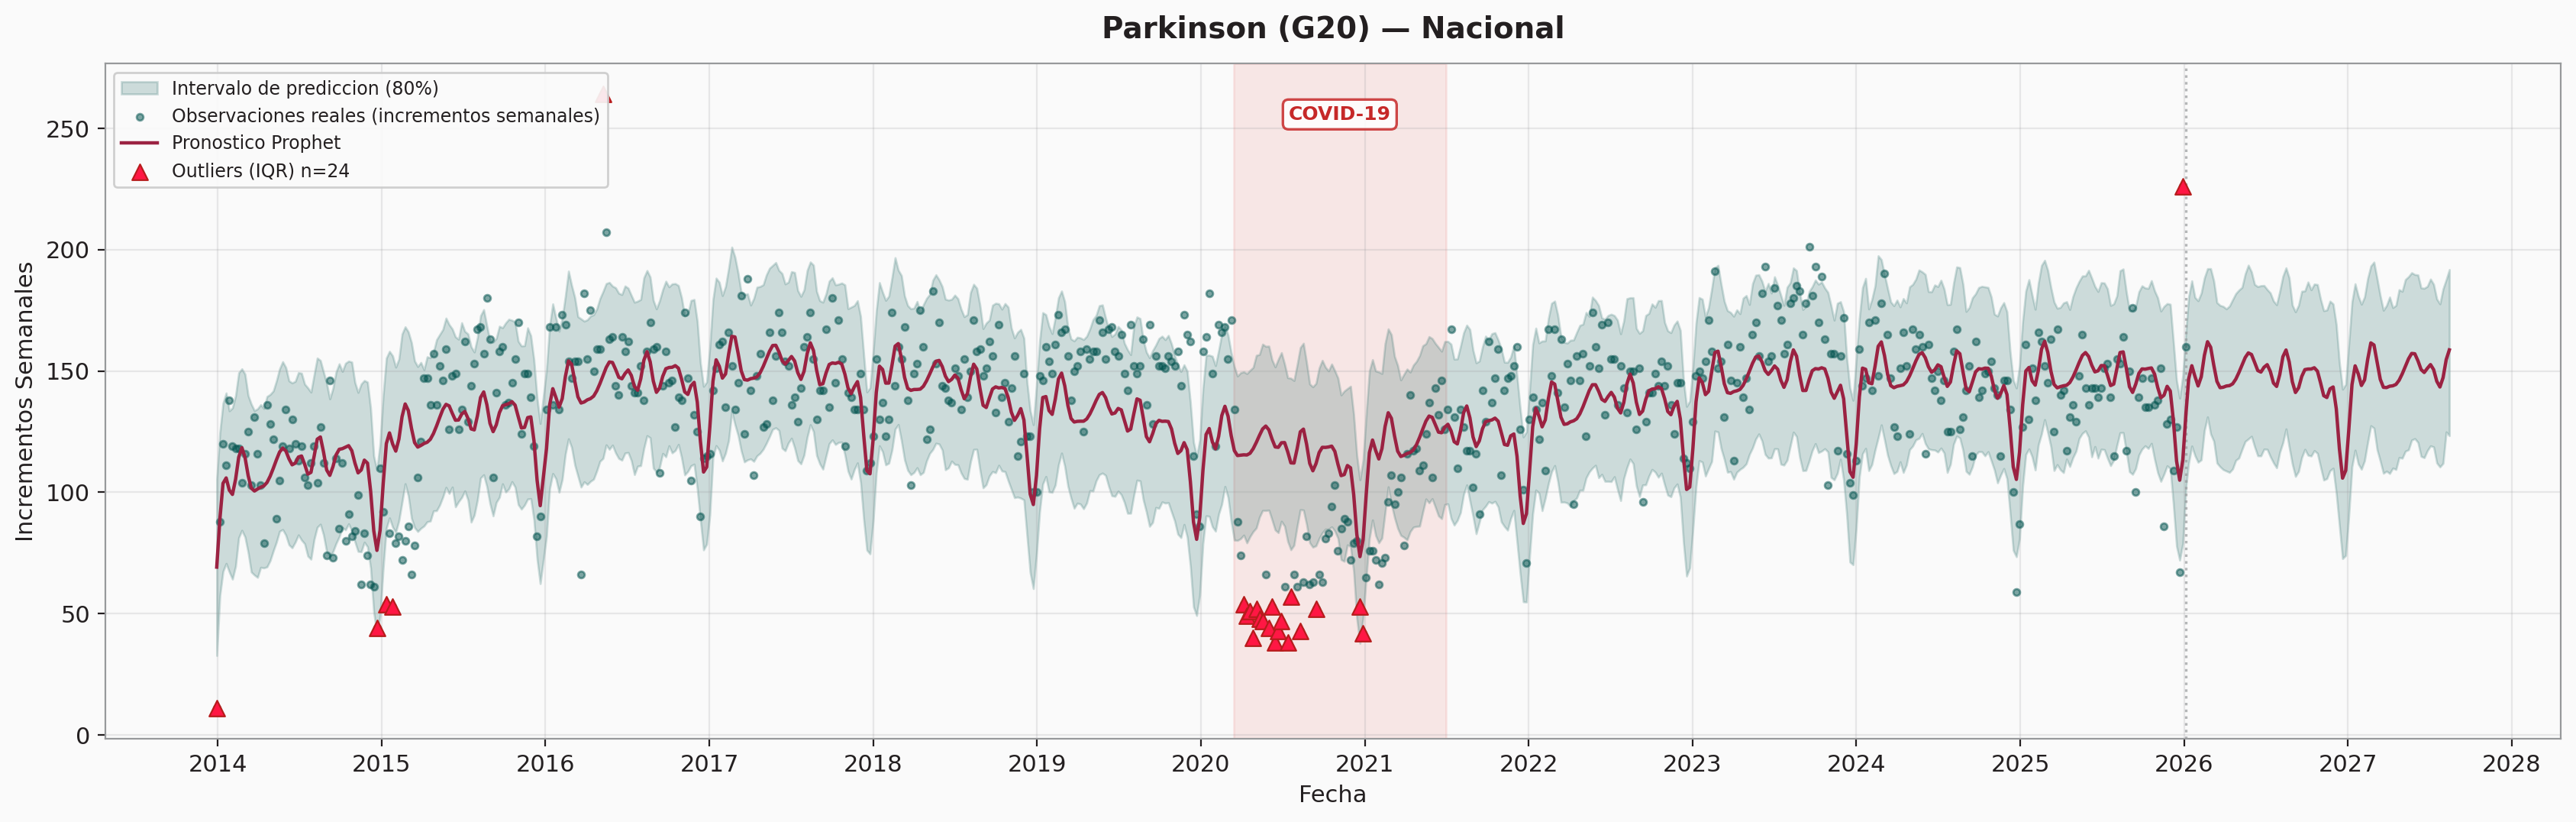
\includegraphics[width=\textwidth]{fig_04_G20_Parkinson_nacional_pronostico.png}
\caption{Pronóstico nacional — Parkinson (G20).}
\label{fig:g20-pronostico}
\end{figure}

\begin{figure}[H]
\centering
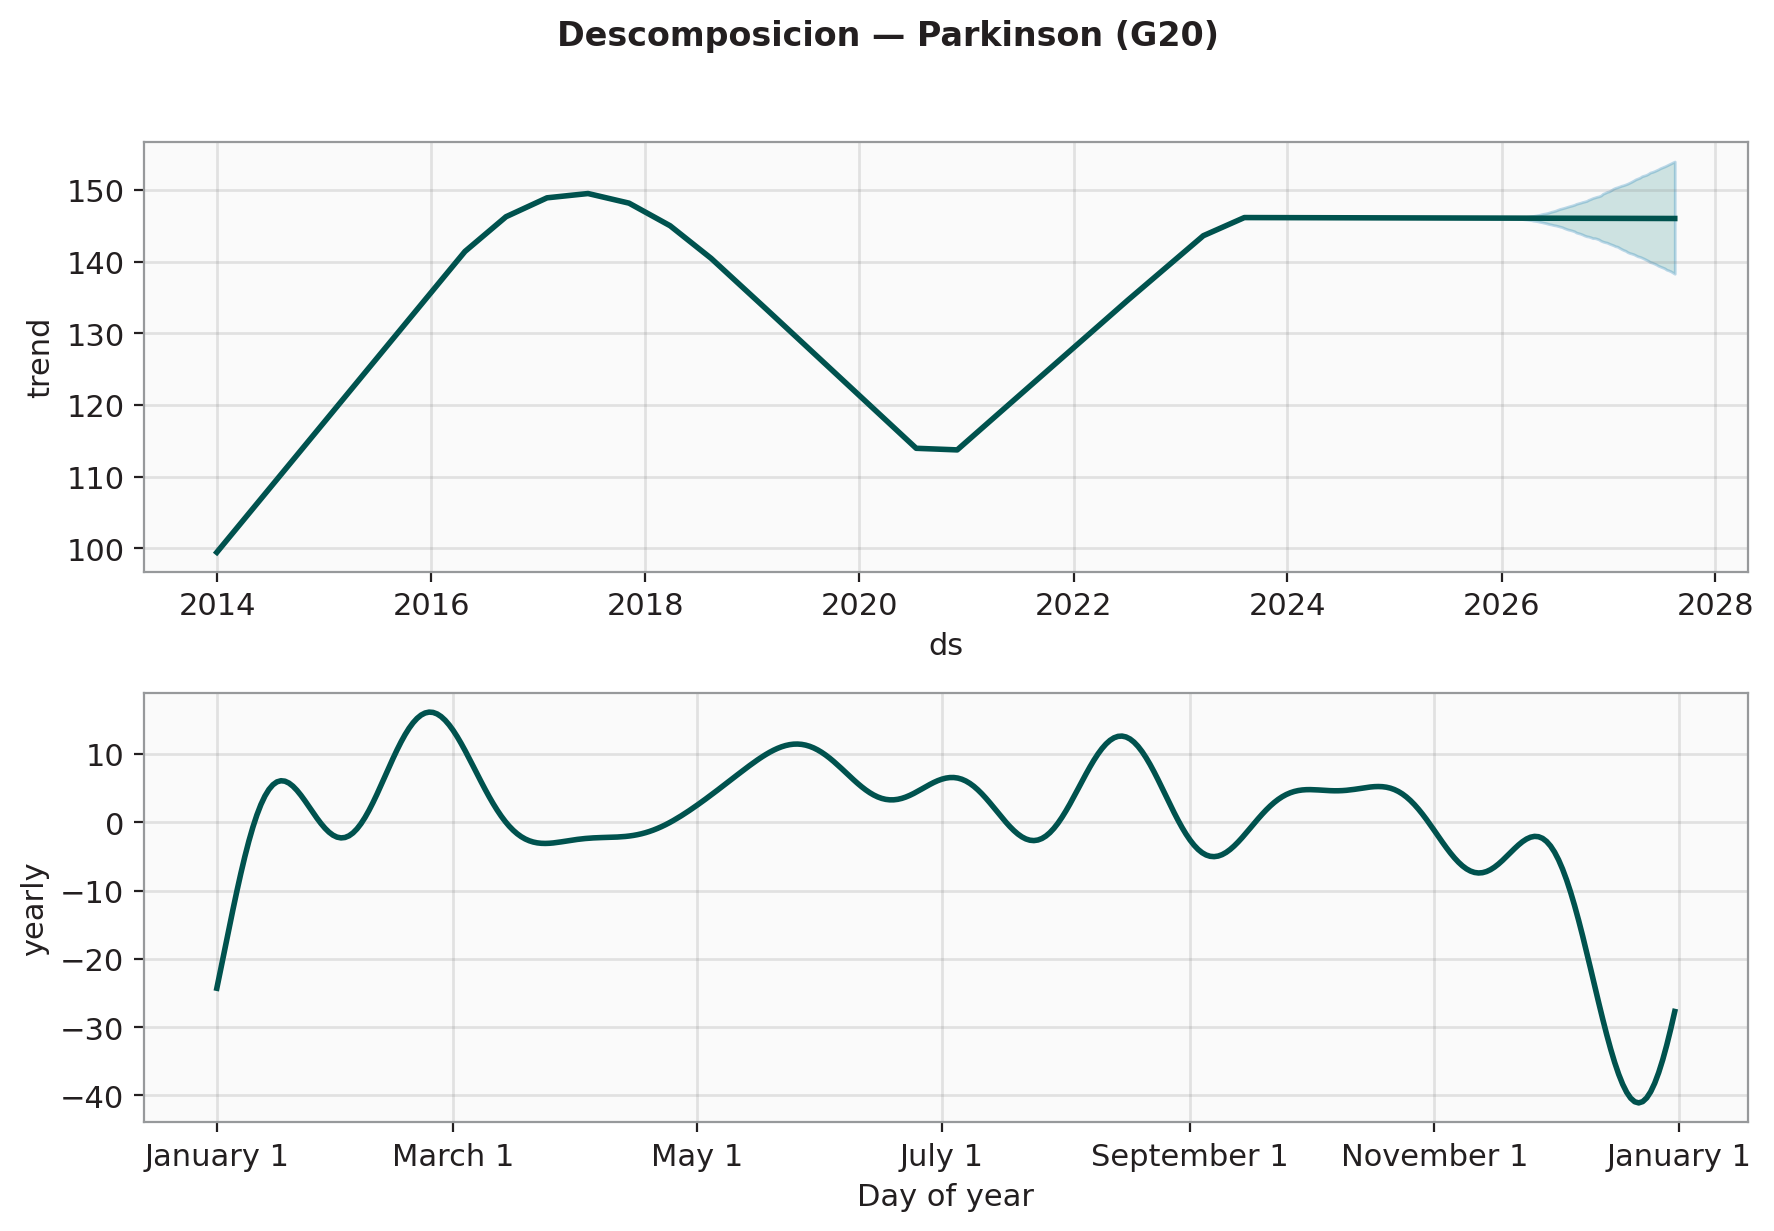
\includegraphics[width=\textwidth]{fig_05_G20_Parkinson_nacional_componentes.png}
\caption{Descomposición en componentes — Parkinson (G20).}
\label{fig:g20-componentes}
\end{figure}

\begin{figure}[H]
\centering
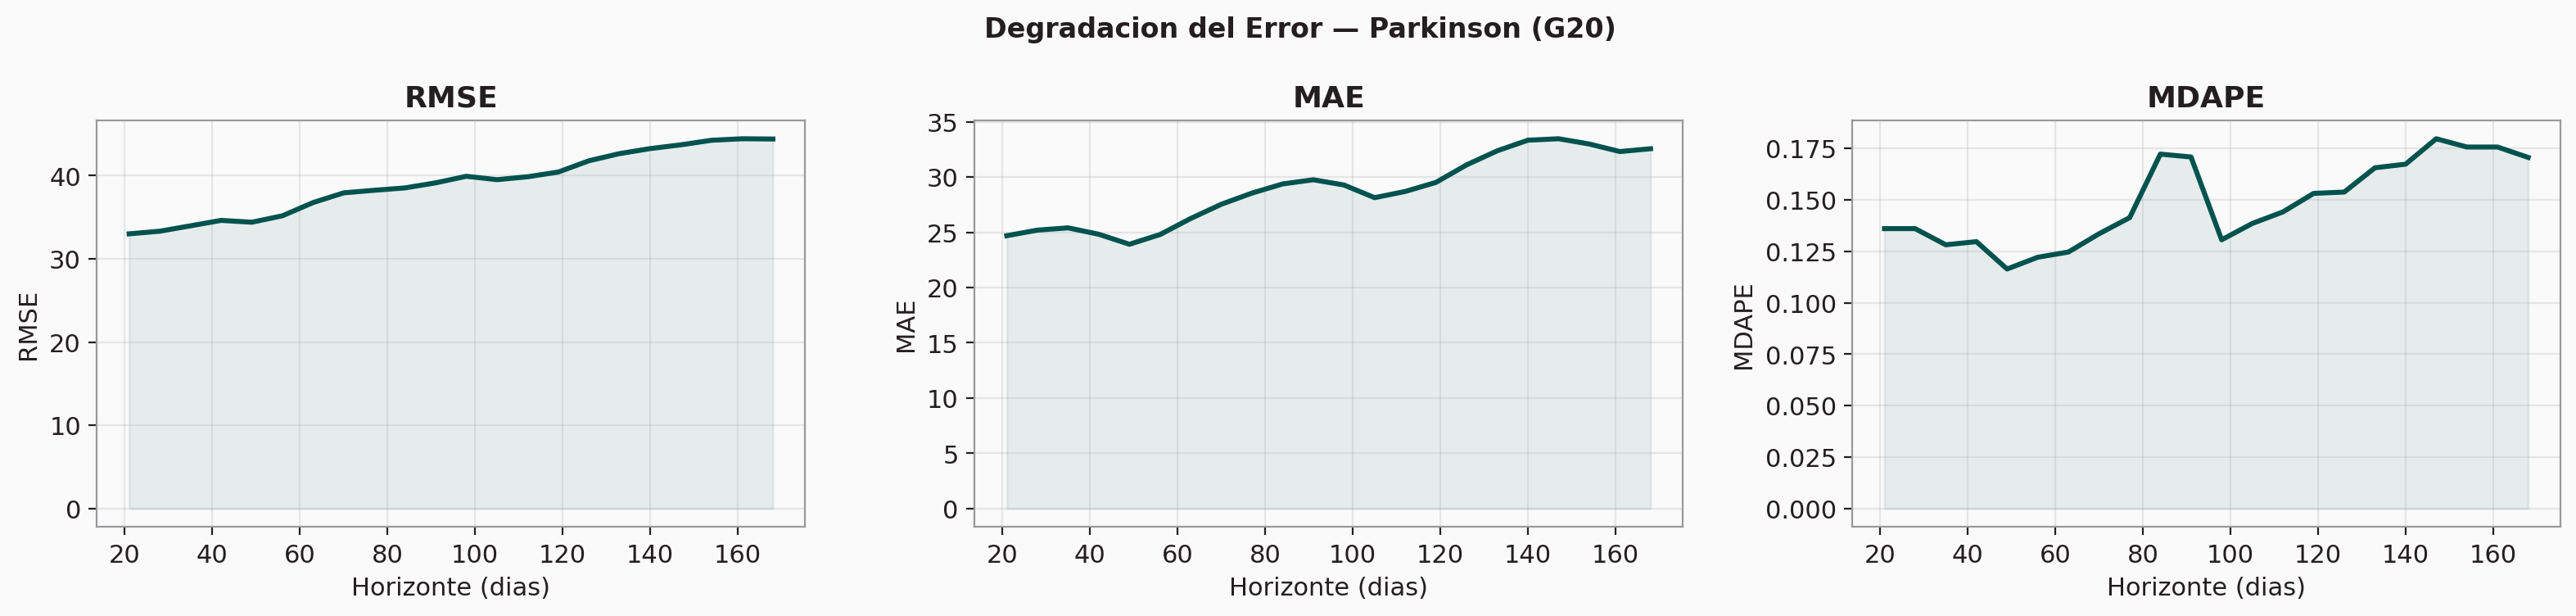
\includegraphics[width=\textwidth]{fig_06_G20_Parkinson_nacional_cv_horizonte.png}
\caption{Degradación del error por horizonte — Parkinson (G20).}
\label{fig:g20-cv}
\end{figure}

\subsection{Alzheimer (G30)}\label{sec:alzheimer}

El modelo nacional de Alzheimer obtuvo un MAPE de 28.30\%, clasificado como \emph{Aceptable}. A diferencia de los otros dos padecimientos, Alzheimer presenta una inversión en la diferencia por sexo: el modelo femenino registra menor error (31.18\%) que el masculino (34.03\%), con una diferencia de $-2.85$ puntos porcentuales. La brecha de sobreajuste es la menor de los tres padecimientos (4.90~pp). No se detectaron outliers en la serie de Alzheimer (0 a nivel estatal), lo cual sugiere series más estables pero con menor señal.

\begin{figure}[H]
\centering
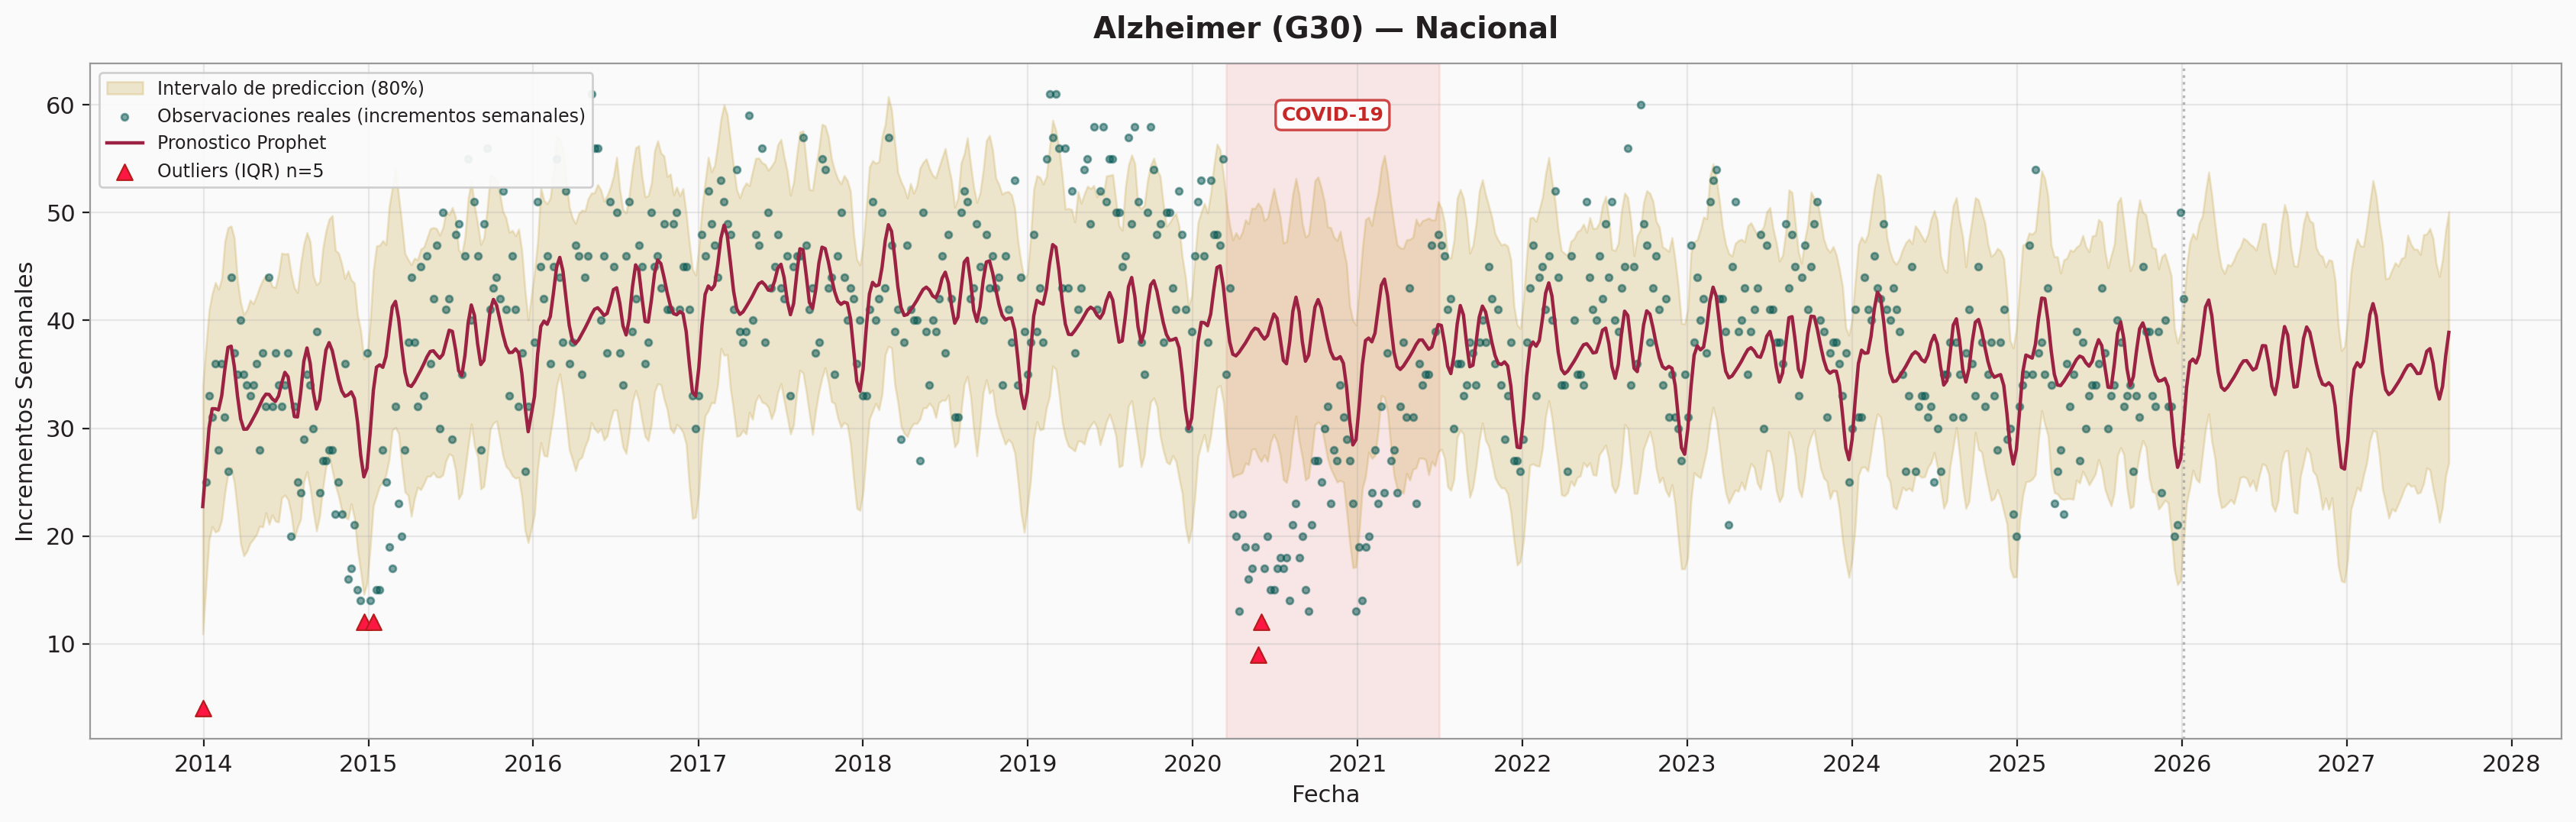
\includegraphics[width=\textwidth]{fig_07_G30_Alzheimer_nacional_pronostico.png}
\caption{Pronóstico nacional — Alzheimer (G30).}
\label{fig:g30-pronostico}
\end{figure}

\begin{figure}[H]
\centering
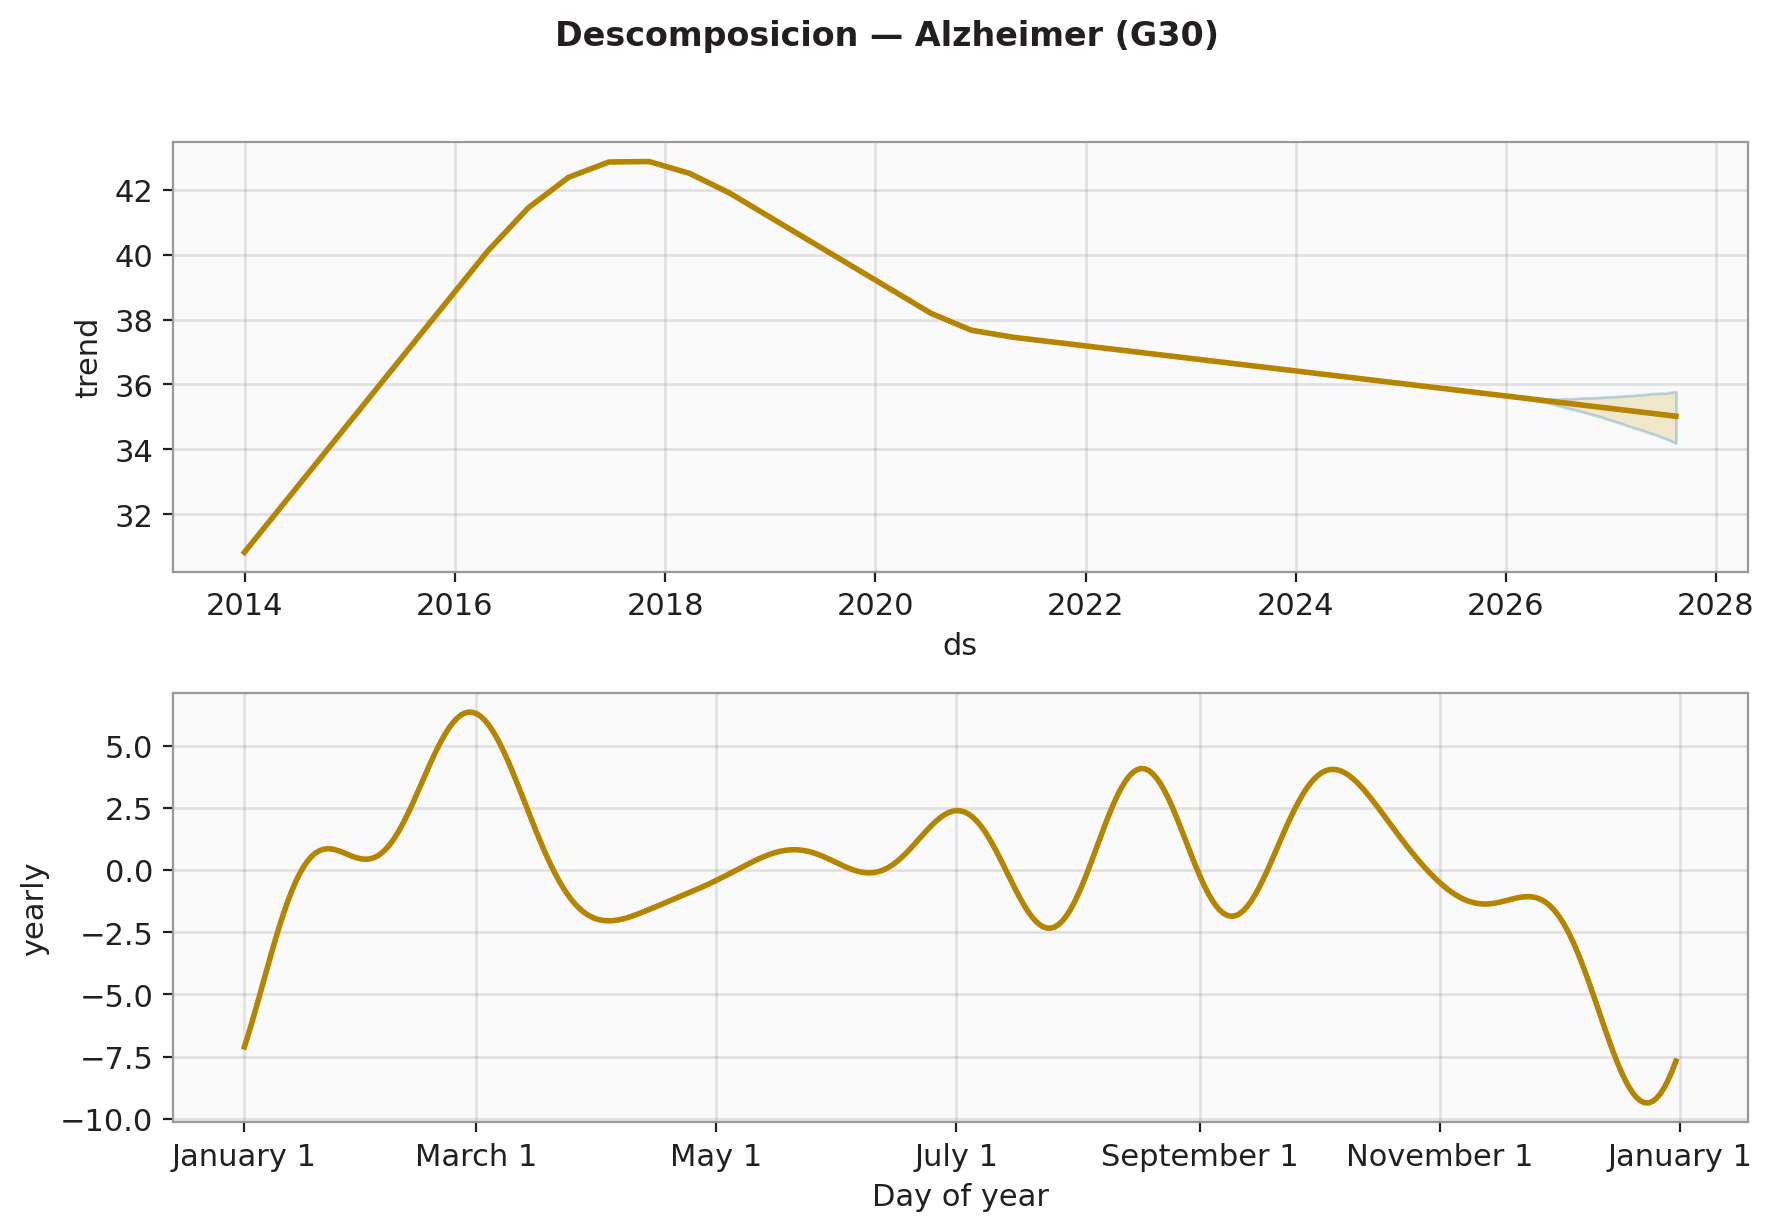
\includegraphics[width=\textwidth]{fig_08_G30_Alzheimer_nacional_componentes.png}
\caption{Descomposición en componentes — Alzheimer (G30).}
\label{fig:g30-componentes}
\end{figure}

\begin{figure}[H]
\centering
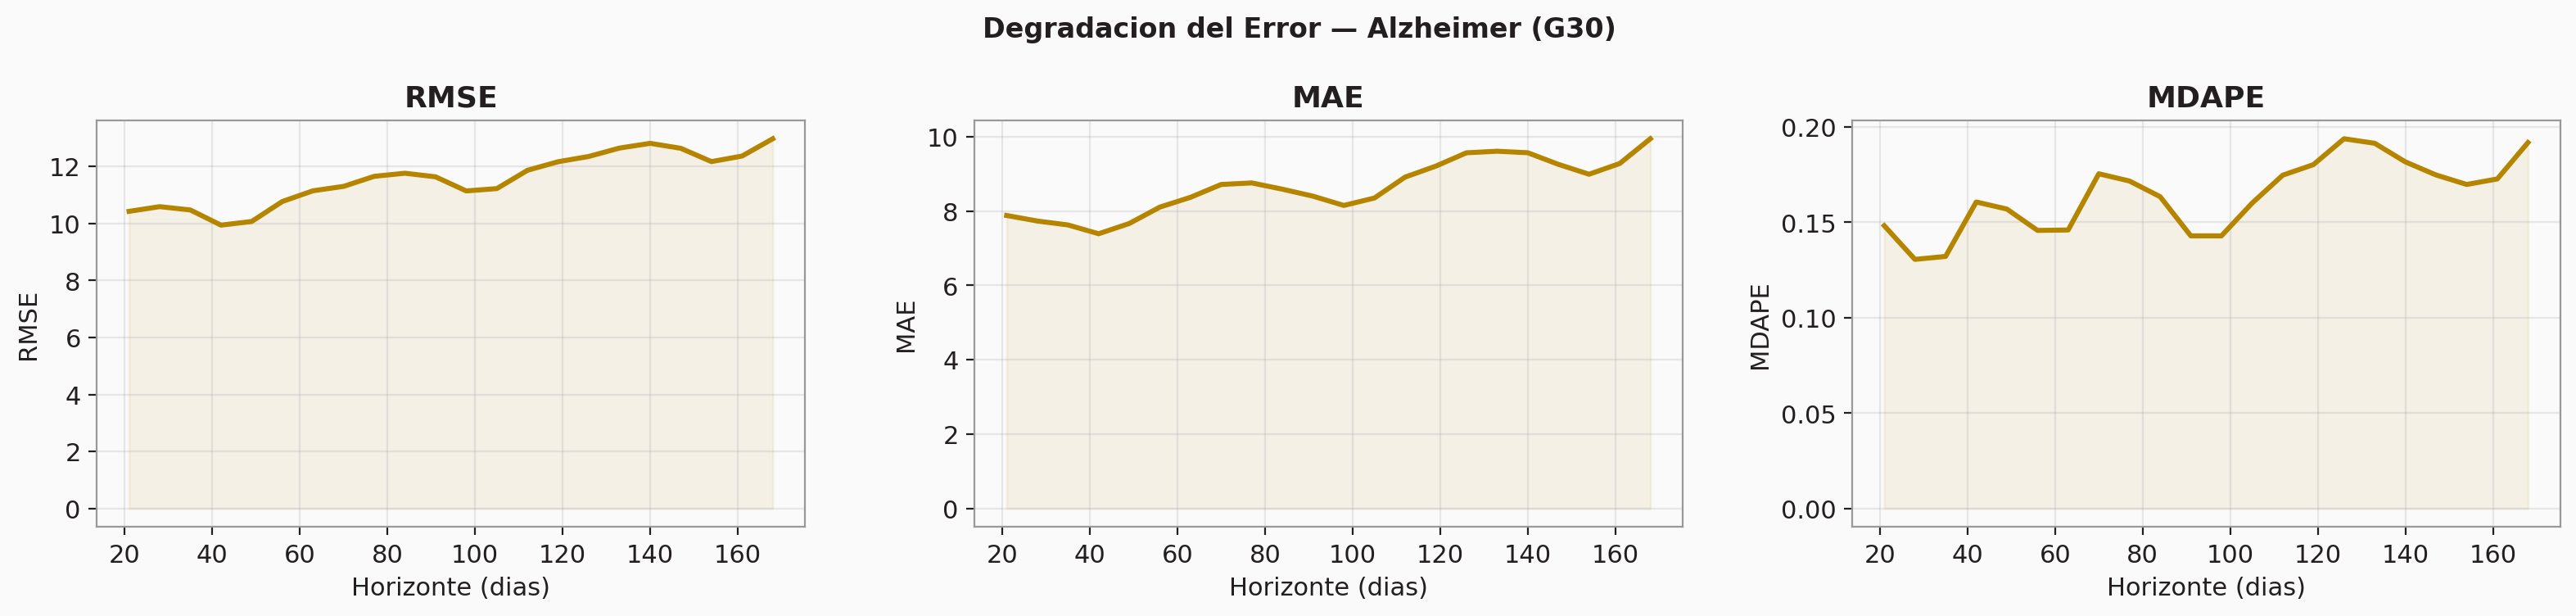
\includegraphics[width=\textwidth]{fig_09_G30_Alzheimer_nacional_cv_horizonte.png}
\caption{Degradación del error por horizonte — Alzheimer (G30).}
\label{fig:g30-cv}
\end{figure}

% =============================================================================
%  4. DASHBOARD EJECUTIVO COMPARATIVO
% =============================================================================
\section{Dashboard Ejecutivo Comparativo}\label{sec:dashboard}

Se construyó un dashboard ejecutivo que permite la comparación visual simultánea de los tres padecimientos en seis paneles (Figura~\ref{fig:dashboard-6paneles}) y un heatmap de desempeño por entidad federativa (Figura~\ref{fig:heatmap}).

\begin{figure}[H]
\centering
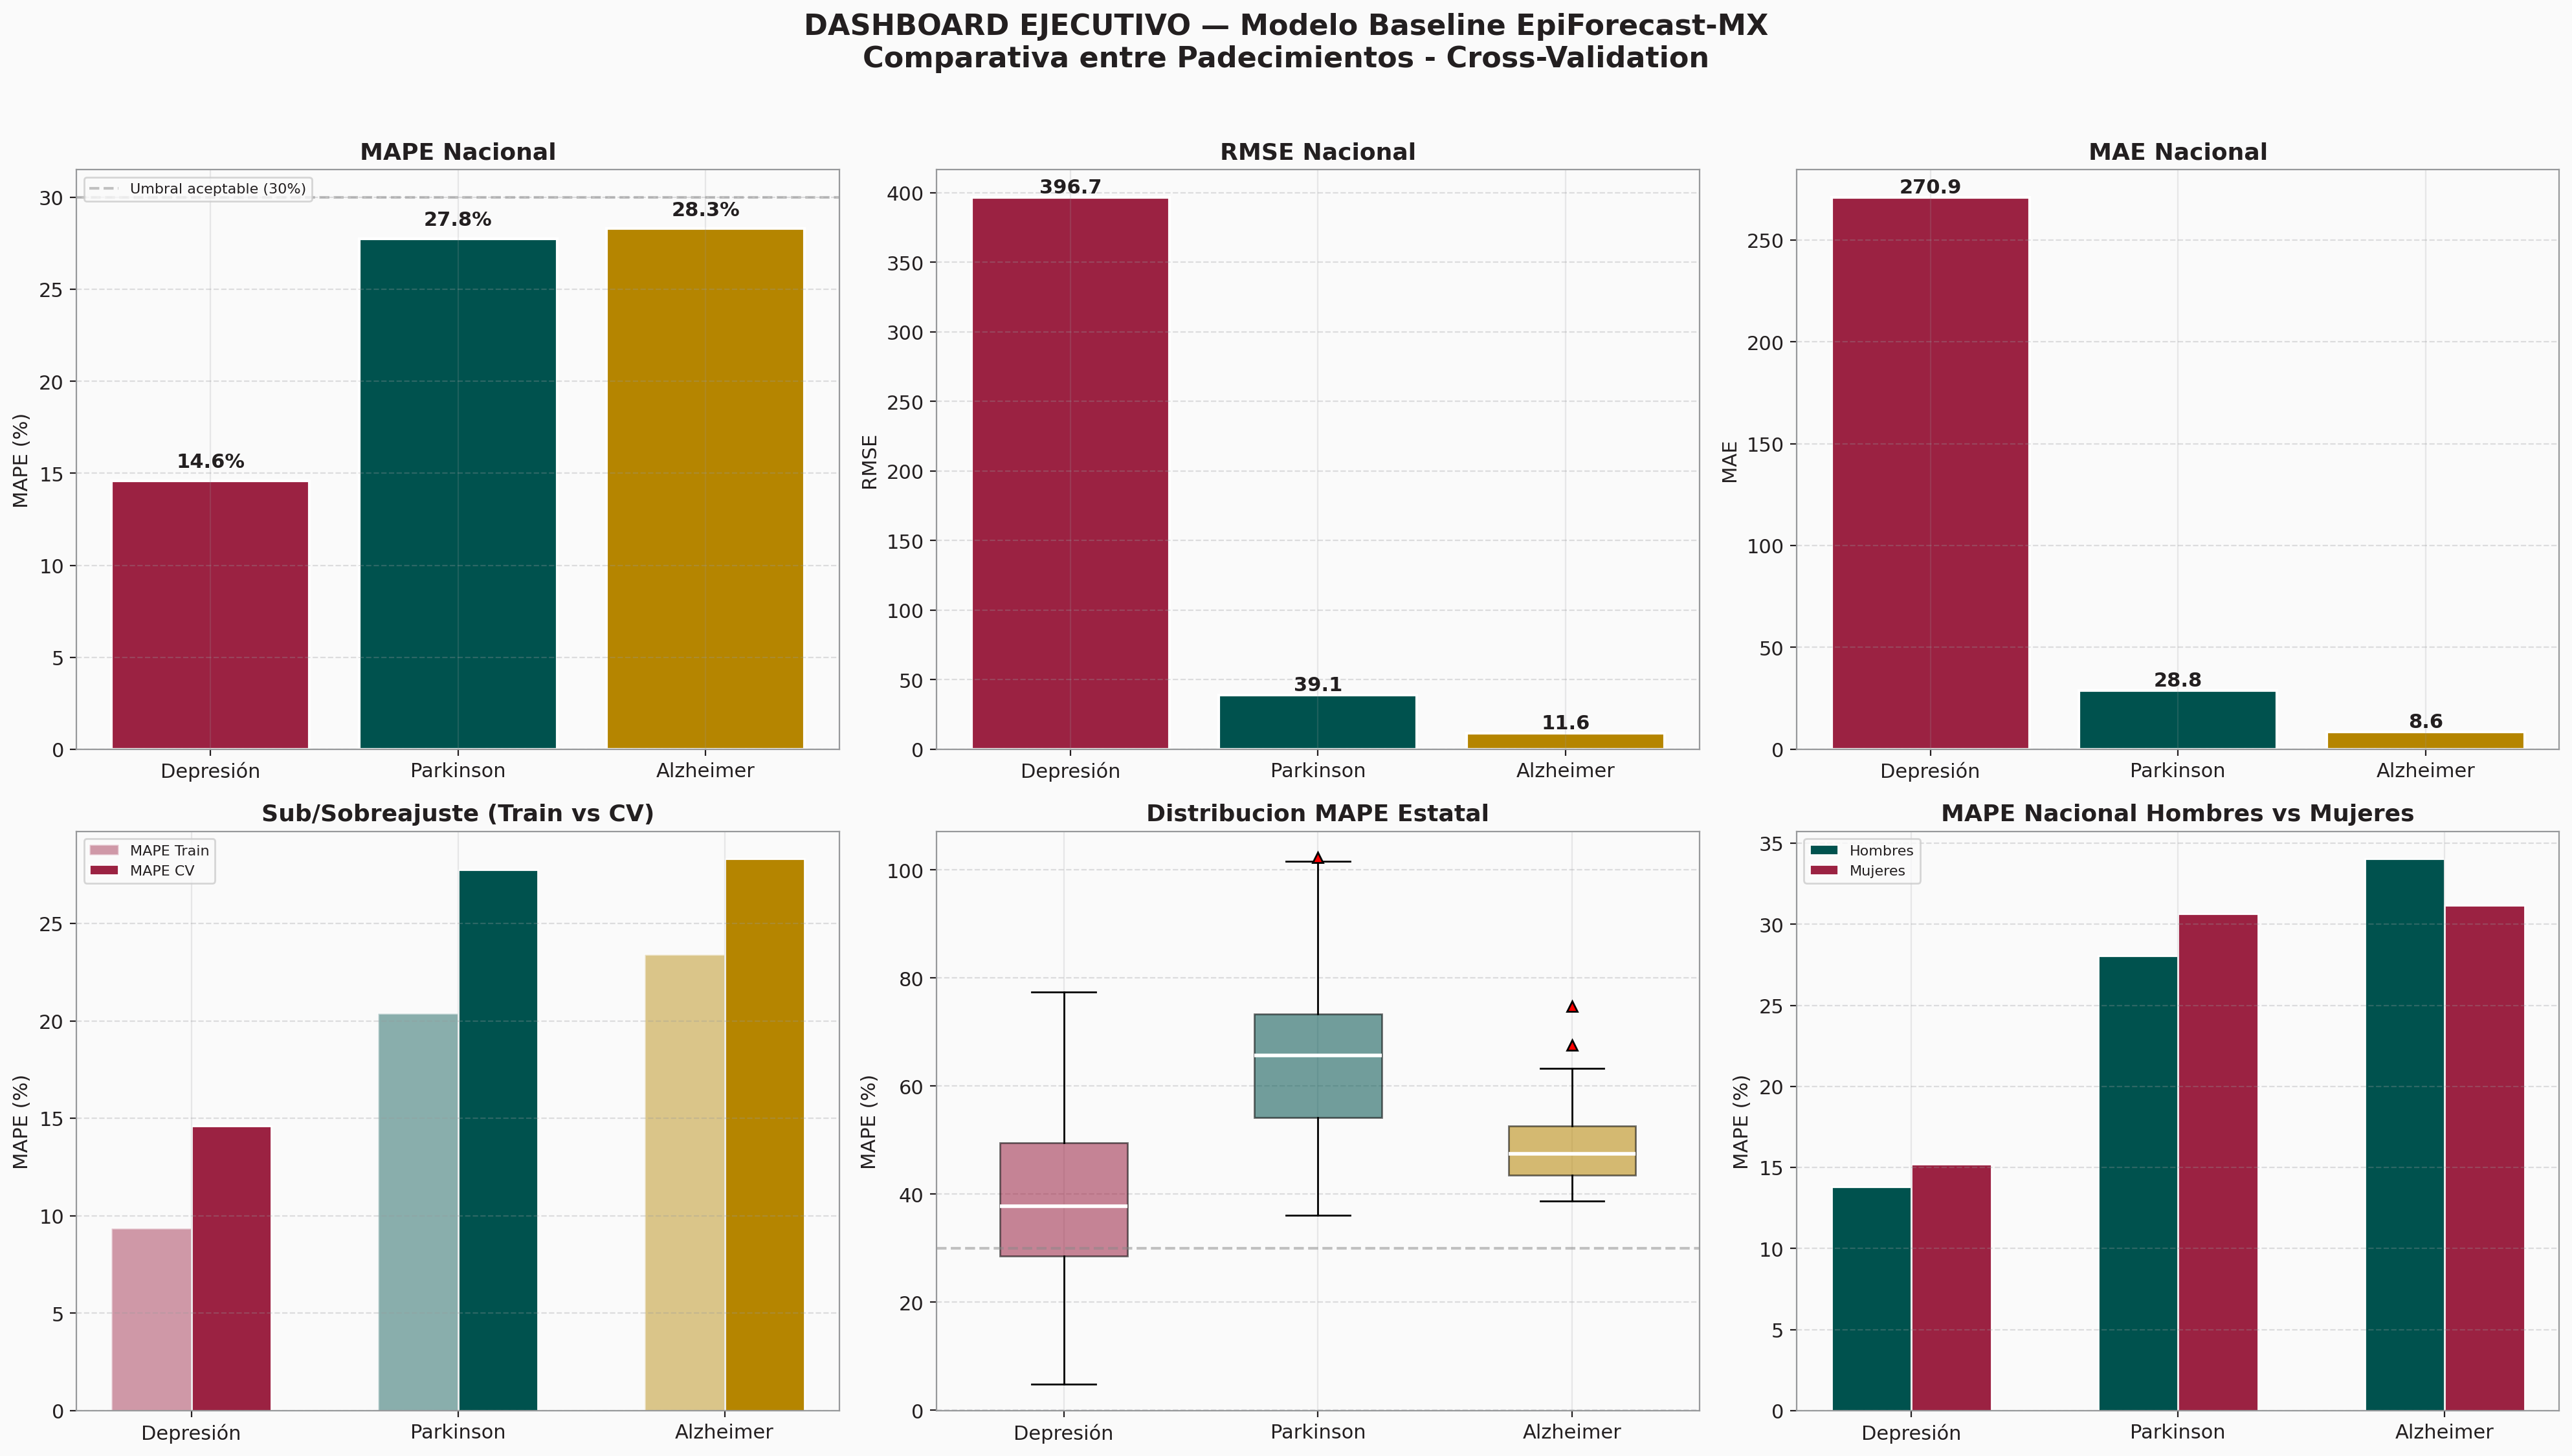
\includegraphics[width=\textwidth]{fig_10_sec09_dashboard_6paneles.png}
\caption{Dashboard ejecutivo — Seis paneles comparativos. Fila superior: distribución del MAPE por estado para cada padecimiento. Fila inferior: comparativas de métricas complementarias.}
\label{fig:dashboard-6paneles}
\end{figure}

\begin{figure}[H]
\centering
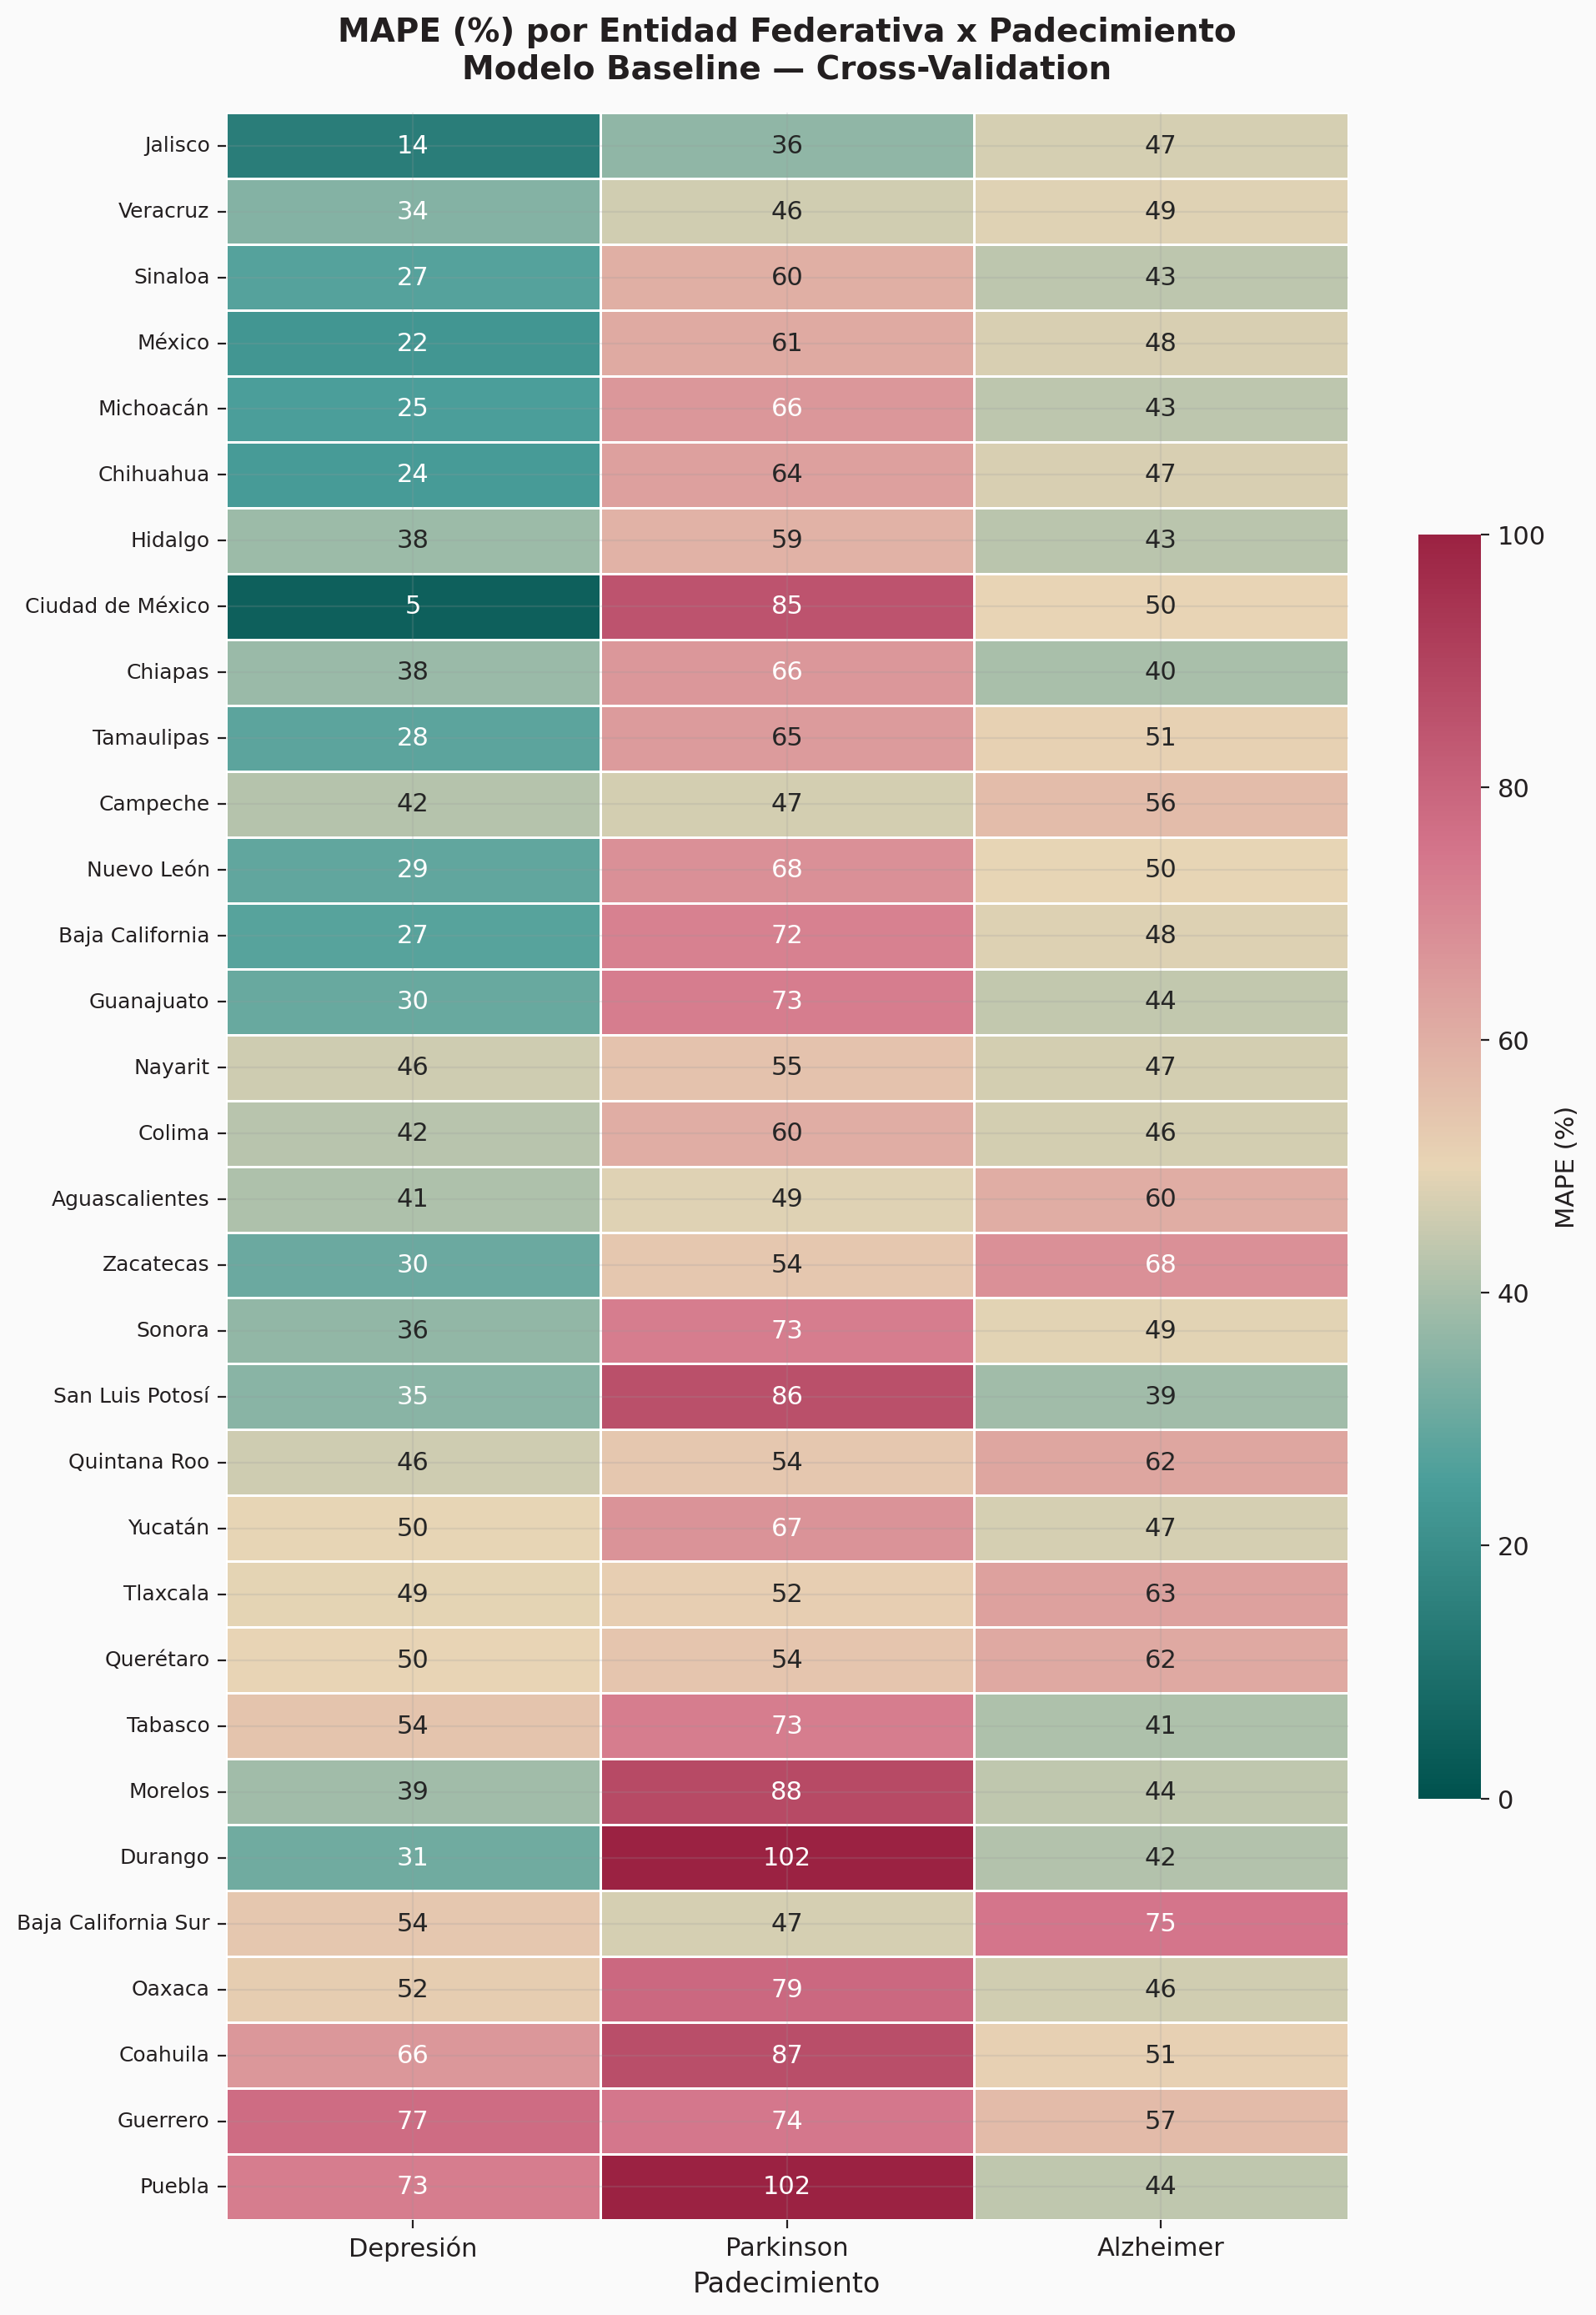
\includegraphics[width=\textwidth]{fig_11_sec09_heatmap_estado_padecimiento.png}
\caption{Heatmap del MAPE por entidad federativa y padecimiento. Tonalidades más oscuras indican mayor error de predicción.}
\label{fig:heatmap}
\end{figure}

La Tabla~\ref{tab:resumen-ejecutivo} sintetiza los indicadores clave extraídos del análisis comparativo de los 297 modelos.

\begin{table}[H]
\centering
\caption{Resumen ejecutivo comparativo de los tres padecimientos.}
\label{tab:resumen-ejecutivo}
\small
\begin{tabular}{@{}l r r r@{}}
\toprule
\textbf{Indicador} & \textbf{Depresión} & \textbf{Parkinson} & \textbf{Alzheimer} \\
\midrule
MAPE Nacional (\%)            & 14.60  & 27.76  & 28.30 \\
RMSE Nacional                 & 396.68 & 39.07  & 11.55 \\
MAPE\textsubscript{train} Nacional (\%) & 9.37 & 20.37 & 23.41 \\
\addlinespace
MAPE Hombres (\%)             & 13.80  & 28.04  & 34.03 \\
MAPE Mujeres (\%)             & 15.21  & 30.64  & 31.18 \\
Dif.\ por sexo (pp)           & 1.41   & 2.60   & $-2.85$ \\
Mejor sexo                    & Hombres & Hombres & Mujeres \\
\addlinespace
Mediana MAPE estatal (\%)     & 37.79  & 65.62  & 47.48 \\
Media MAPE estatal (\%)       & 39.22  & 66.32  & 50.05 \\
Desv.\ est.\ MAPE estatal    & 15.80  & 15.95  & 8.60 \\
Mín.\ MAPE estatal (\%)      & 4.79   & 36.04  & 38.69 \\
Máx.\ MAPE estatal (\%)      & 77.43  & 102.27 & 74.74 \\
\addlinespace
Mejor estado                  & Cd.\ de México & Jalisco & San Luis Potosí \\
Peor estado                   & Guerrero & Puebla & Baja Calif.\ Sur \\
\addlinespace
Total de modelos              & 99     & 99     & 99 \\
Outliers totales              & 143    & 36     & 0 \\
\bottomrule
\end{tabular}
\end{table}

% =============================================================================
%  5. ANÁLISIS DE SUB/SOBREAJUSTE
% =============================================================================
\section{Análisis de Sub/Sobreajuste}\label{sec:subsobreajuste}

La Figura~\ref{fig:scatter-ajuste} presenta el diagrama de dispersión del MAPE de entrenamiento contra el MAPE de validación cruzada para cada modelo estatal. Los puntos ubicados sobre la diagonal ($y = x$) indican mayor error en validación que en entrenamiento, lo cual es la condición esperada en modelos correctamente regularizados. Puntos significativamente por encima sugieren sobreajuste, mientras que puntos sobre o debajo de la diagonal con valores altos en ambos ejes sugieren subajuste.

\begin{figure}[H]
\centering
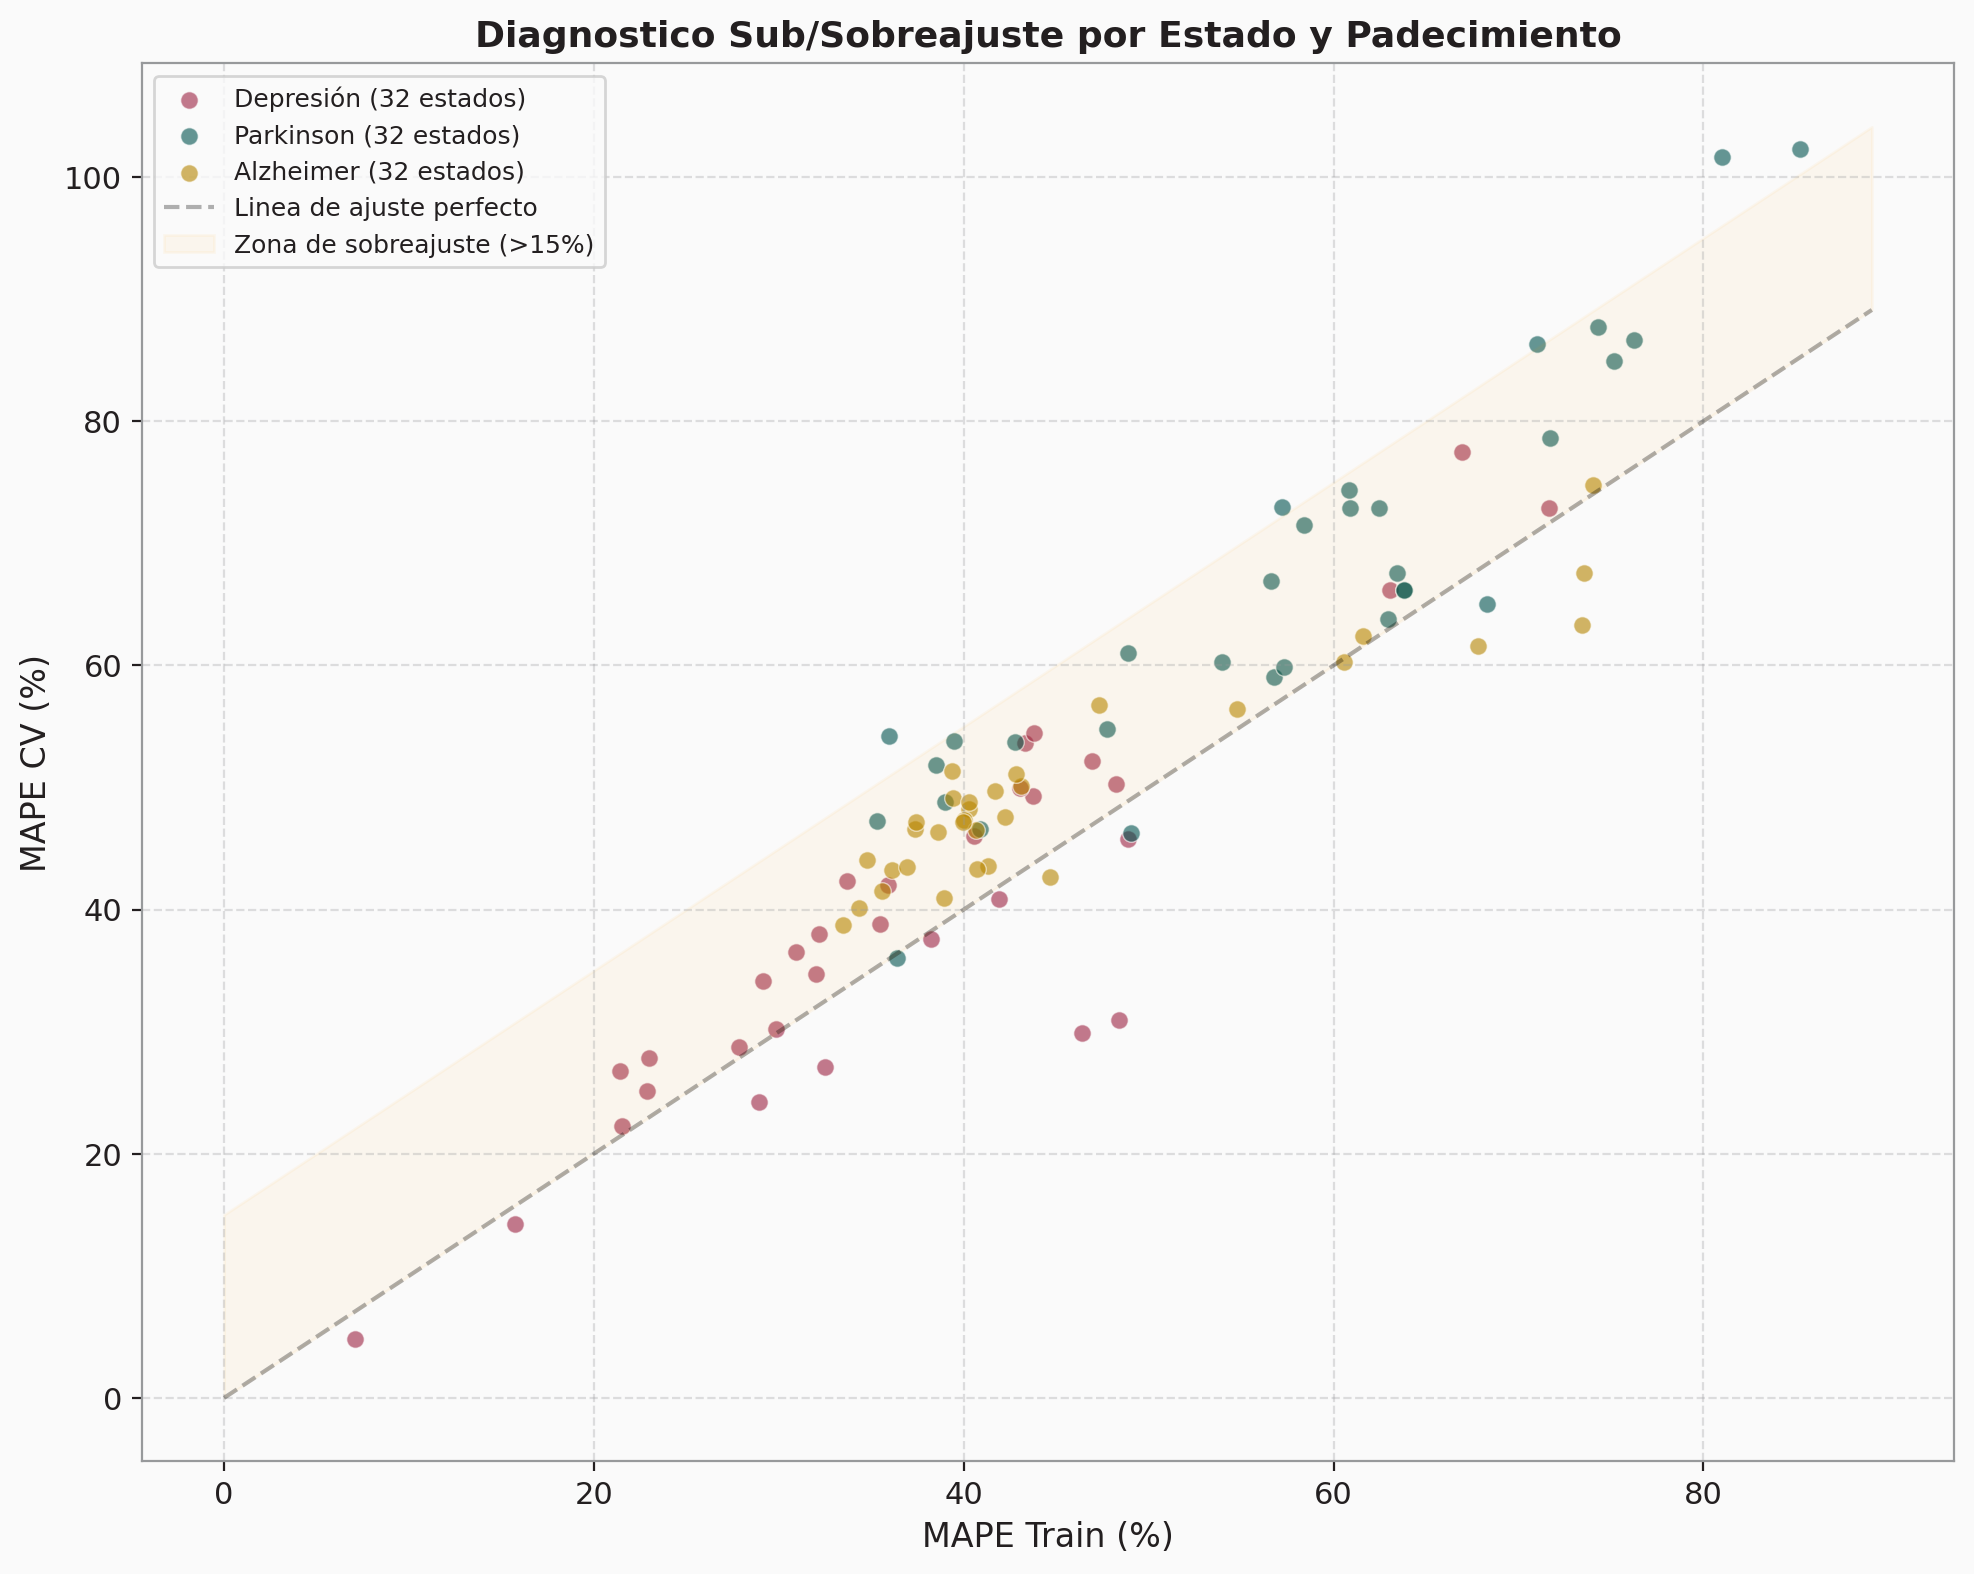
\includegraphics[width=0.85\textwidth]{fig_12_sec10_scatter_subsobreajuste.png}
\caption{Diagnóstico de sub/sobreajuste por estado y padecimiento. Puntos sobre la diagonal indican mayor error en validación que en entrenamiento.}
\label{fig:scatter-ajuste}
\end{figure}

La Tabla~\ref{tab:brechas} presenta las brechas promedio entre entrenamiento y validación a nivel nacional. Una brecha positiva indica que el error de validación es mayor que el de entrenamiento (comportamiento esperado); brechas excesivamente grandes sugieren sobreajuste.

\begin{table}[H]
\centering
\caption{Brechas MAPE\textsubscript{CV} $-$ MAPE\textsubscript{train} a nivel nacional.}
\label{tab:brechas}
\begin{tabular}{@{}l r r r@{}}
\toprule
\textbf{Padecimiento / Nivel} & \textbf{MAPE\textsubscript{CV} (\%)} & \textbf{MAPE\textsubscript{train} (\%)} & \textbf{Brecha (pp)} \\
\midrule
Depresión — Nacional & 14.60 & 9.37 & 5.22 \\
Depresión — Hombres  & 13.80 & 9.58 & 4.22 \\
Depresión — Mujeres  & 15.21 & 10.06 & 5.15 \\
\addlinespace
Parkinson — Nacional & 27.76 & 20.37 & 7.39 \\
Parkinson — Hombres  & 28.04 & 22.78 & 5.27 \\
Parkinson — Mujeres  & 30.64 & 23.31 & 7.34 \\
\addlinespace
Alzheimer — Nacional & 28.30 & 23.41 & 4.90 \\
Alzheimer — Hombres  & 34.03 & 28.85 & 5.18 \\
Alzheimer — Mujeres  & 31.18 & 27.19 & 3.99 \\
\bottomrule
\end{tabular}
\end{table}

Las brechas oscilan entre 3.99 y 7.39 puntos porcentuales. Parkinson presenta las brechas más amplias (hasta 7.39~pp a nivel nacional y 7.34~pp en mujeres), lo cual es consistente con el menor volumen de datos disponibles para este padecimiento. Alzheimer muestra la menor brecha global (3.99~pp en mujeres), sugiriendo que los patrones de esta serie son menos propensos al sobreajuste a nivel nacional, aunque el error absoluto sigue siendo elevado.

% =============================================================================
%  6. ANÁLISIS DE COMPONENTES
% =============================================================================
\section{Análisis de Componentes}\label{sec:componentes}

En Prophet, el modelo aditivo se expresa como:
\begin{equation}
\hat{y}(t) = g(t) + s(t) + \epsilon_t
\label{eq:prophet-model}
\end{equation}
donde $g(t)$ representa la tendencia (evolución estructural a largo plazo), $s(t)$ la estacionalidad anual (patrones cíclicos de 52~semanas) y $\epsilon_t$ el término de error \citep{taylor2018forecasting}. A diferencia de modelos supervisados donde la importancia se asigna a \emph{features} explícitas, Prophet opera sobre descomposición temporal, por lo que las ``características'' relevantes son los componentes del modelo.

La Tabla~\ref{tab:componentes} presenta la contribución relativa de cada componente a la varianza explicada del modelo y los \emph{changepoints} detectados durante el período COVID-19.

\begin{table}[H]
\centering
\caption{Contribución de varianza por componente y \emph{changepoints} COVID-19.}
\label{tab:componentes}
\resizebox{\textwidth}{!}{%
\begin{tabular}{@{}l r r c c l@{}}
\toprule
\textbf{Padecimiento} & \textbf{Tendencia (\%)} & \textbf{Estacionalidad (\%)} & \textbf{Changepoints} & \textbf{CP COVID} & \textbf{Fechas COVID} \\
\midrule
Depresión & 82.4 & 17.6 & 25 & 5 & 2020-02-24; 2020-07-13; 2020-11-30; 2021-04-19; 2021-09-06 \\
Parkinson & 60.3 & 39.7 & 25 & 5 & 2020-02-24; 2020-07-13; 2020-11-30; 2021-04-19; 2021-09-06 \\
Alzheimer & 45.6 & 54.4 & 25 & 5 & 2020-02-24; 2020-07-13; 2020-11-30; 2021-04-19; 2021-09-06 \\
\bottomrule
\end{tabular}%
}
\end{table}
\begin{figure}[H]
\centering
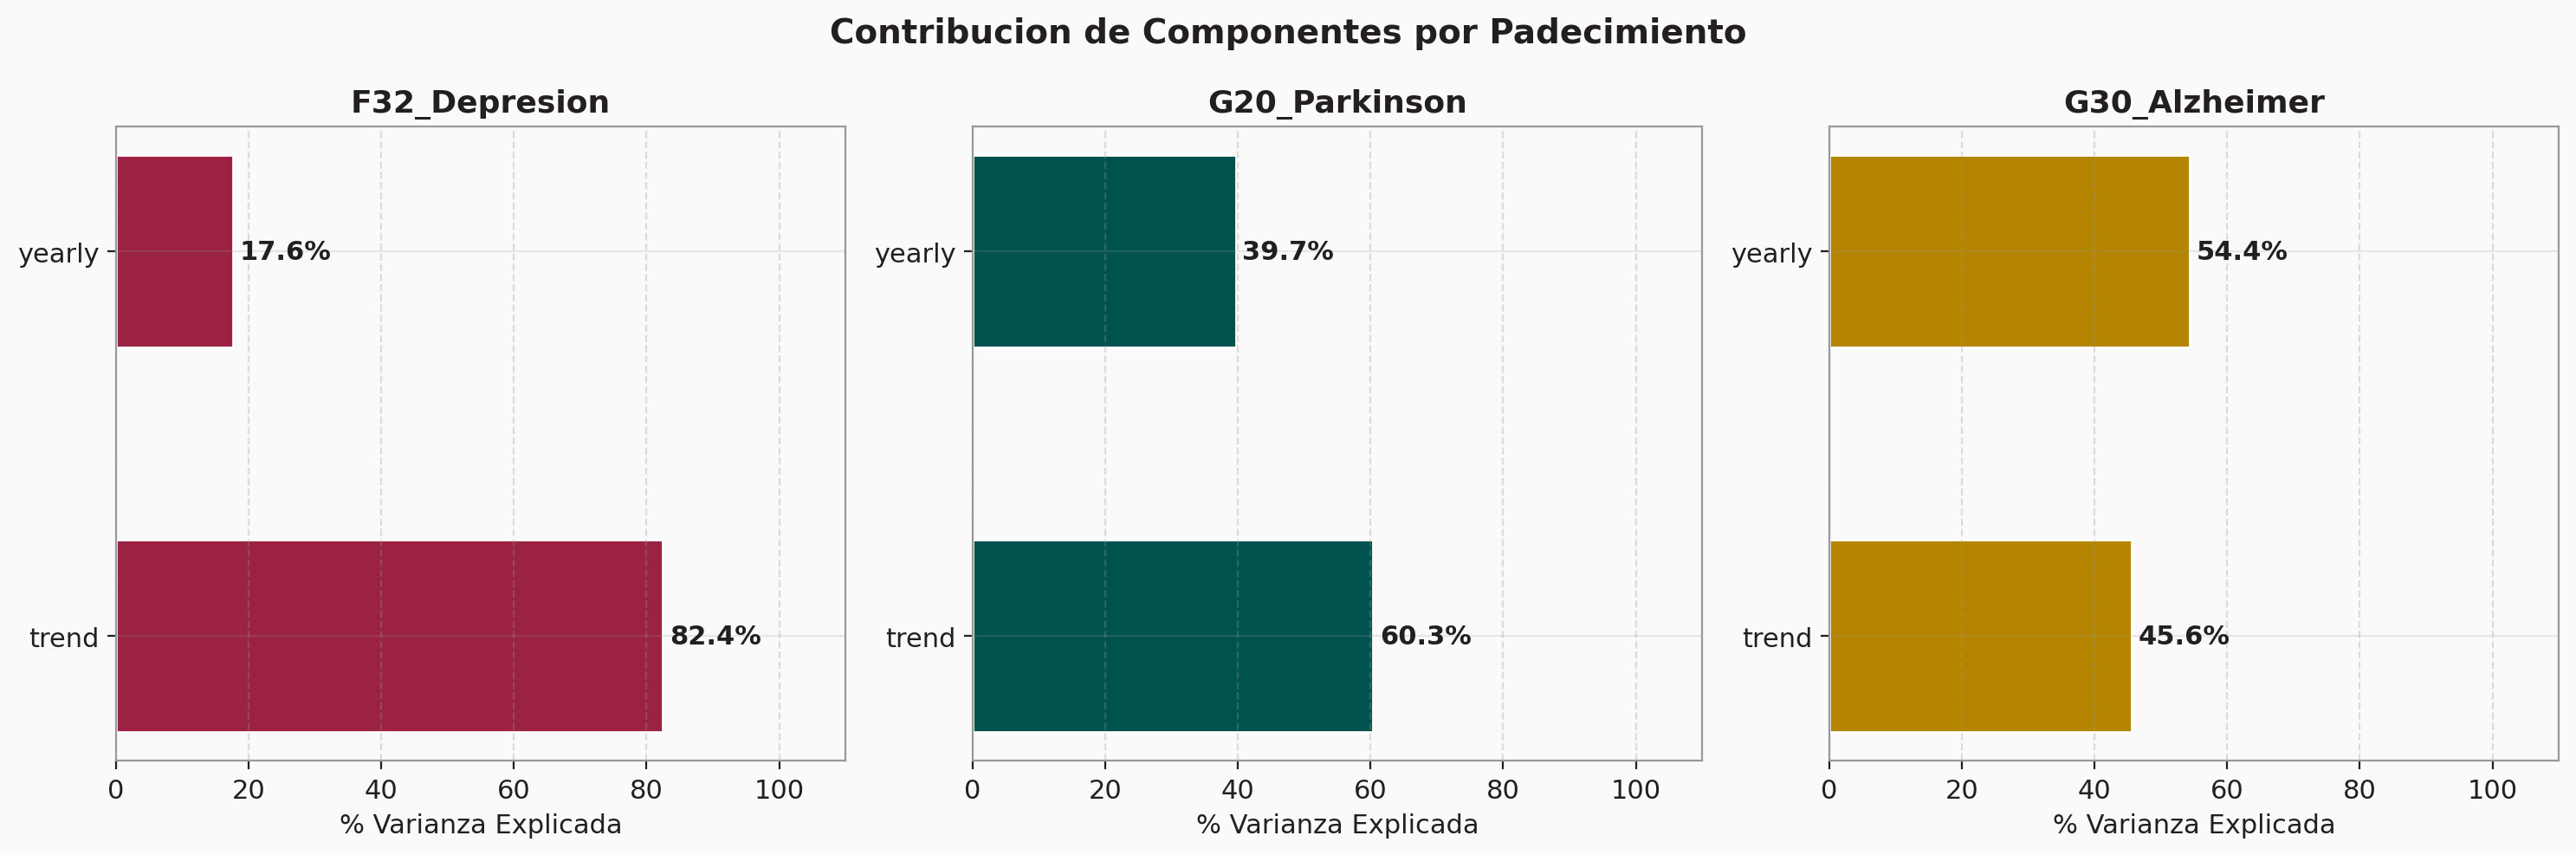
\includegraphics[width=0.85\textwidth]{fig_13_sec11_varianza_componentes.png}
\caption{Contribución de varianza por componente para cada padecimiento.}
\label{fig:varianza-componentes}
\end{figure}

El análisis revela patrones diferenciados entre padecimientos. En Depresión, la tendencia domina con un 82.4\% de la varianza, lo que indica una evolución estructural pronunciada (incremento sostenido en consultas de salud mental a lo largo de la década). Parkinson muestra un balance más equilibrado (60.3\%/39.7\%), reflejando tanto una tendencia ascendente moderada como una estacionalidad relevante. Alzheimer presenta una inversión notable: la estacionalidad explica el 54.4\% de la varianza frente al 45.6\% de la tendencia, sugiriendo que los patrones cíclicos son el principal motor de la variabilidad en las consultas de esta enfermedad.

Los cinco \emph{changepoints} detectados durante el período COVID-19 (2020-02-24, 2020-07-13, 2020-11-30, 2021-04-19 y 2021-09-06) coinciden con las fases del confinamiento en México, validando la capacidad de Prophet para capturar quiebres estructurales. La caída en reportes durante la pandemia —particularmente en Alzheimer— refleja menor detección, no menor prevalencia, tal como señaló la Dra.\ Ruth Pérez en reunión del 11 de febrero de 2026.

% =============================================================================
%  7. DESEMPEÑO MÍNIMO ACEPTABLE
% =============================================================================
\section{Desempeño Mínimo Aceptable}\label{sec:desempeno}

No existe antecedente histórico de pronóstico epidemiológico automatizado para estos padecimientos en el IMSS. Los umbrales se establecieron con base en la literatura \citep{hyndman2021forecasting} y los requisitos institucionales de la Dra.\ Ruth Pérez:

\begin{table}[H]
\centering
\caption{Umbrales de desempeño mínimo aceptable (MAPE).}
\label{tab:umbrales}
\begin{tabular}{@{}l c l@{}}
\toprule
\textbf{Nivel} & \textbf{MAPE} & \textbf{Interpretación} \\
\midrule
Excelente & $\leq 20\%$ & Pronóstico confiable para decisiones operativas \\
Aceptable & $\leq 30\%$ & Útil para planificación estratégica \\
Requiere mejora & $\leq 50\%$ & Indicativo de viabilidad; requiere tuning en Avance~4 \\
Insuficiente & $> 50\%$ & No viable sin mejora significativa \\
\bottomrule
\end{tabular}
\end{table}

La Tabla~\ref{tab:semaforo} presenta la distribución de los 32 estados por categoría de semáforo para cada padecimiento.

\begin{table}[H]
\centering
\caption{Distribución de entidades federativas por semáforo de desempeño.}
\label{tab:semaforo}
\begin{tabular}{@{}l r r r r@{}}
\toprule
\textbf{Padecimiento} & \textbf{Excelente} & \textbf{Aceptable} & \textbf{Requiere mejora} & \textbf{Insuficiente} \\
 & ($\leq$20\%) & ($\leq$30\%) & ($\leq$50\%) & ($>$50\%) \\
\midrule
Depresión & 2 & 8 & 15 & 7 \\
Parkinson & 0 & 0 & 5 & 27 \\
Alzheimer & 0 & 0 & 21 & 11 \\
\bottomrule
\end{tabular}
\end{table}

Depresión es el padecimiento con mejor distribución: 10 estados (31.3\%) se ubican en categorías \emph{Excelente} o \emph{Aceptable}, y solo 7 (21.9\%) resultan \emph{Insuficientes}. En contraste, Parkinson presenta el escenario más desafiante con 27 de 32 estados (84.4\%) clasificados como \emph{Insuficientes} y ningún estado en las categorías superiores. Alzheimer se encuentra en una posición intermedia con 21 estados (65.6\%) en \emph{Requiere mejora} y 11 (34.4\%) \emph{Insuficientes}. Estos resultados confirman la necesidad del tuning de hiperparámetros previsto para el Avance~4, particularmente para Parkinson y Alzheimer a nivel estatal.

% =============================================================================
%  8. GALERÍA COMPARATIVA
% =============================================================================
\section{Galería Comparativa de Modelos}\label{sec:galeria}

\subsection{Comparativa Nacional — Tres Padecimientos}\label{sec:triptych}

La Figura~\ref{fig:triptych} presenta el tríptico nacional que permite la comparación visual directa de los tres padecimientos.

\begin{figure}[H]
\centering
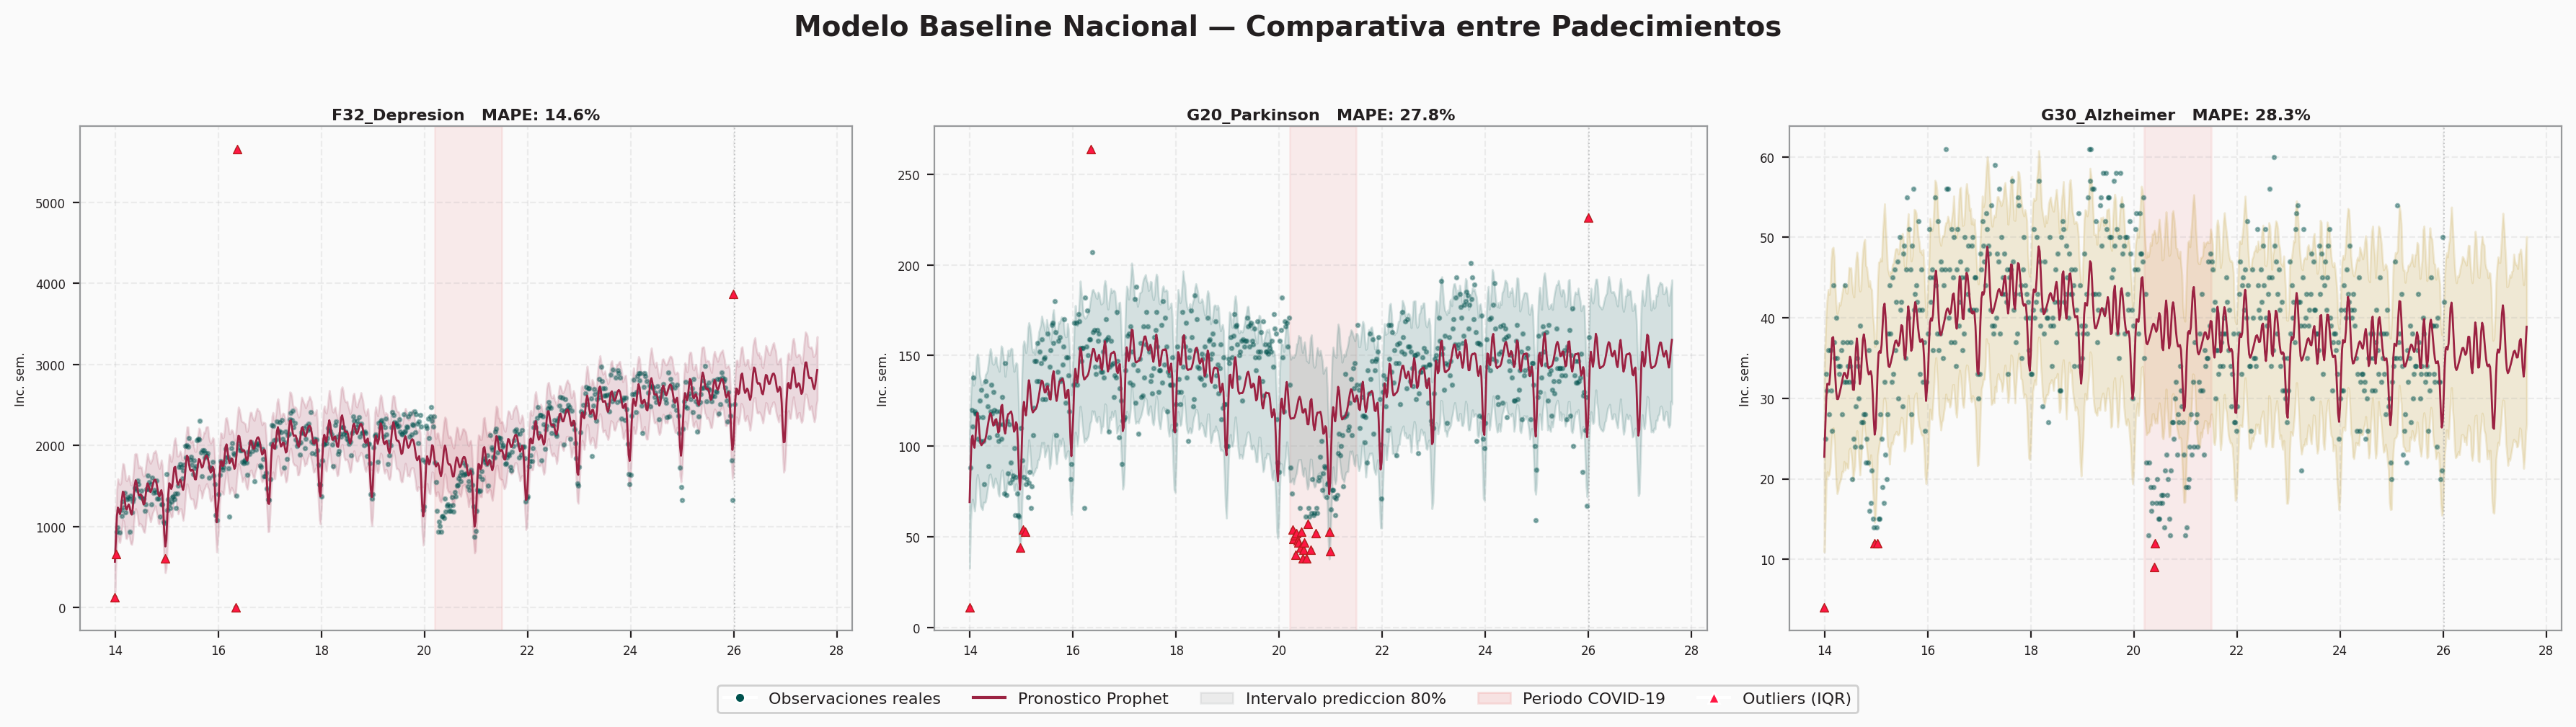
\includegraphics[width=\textwidth]{fig_14_sec13_1_triptych_nacional.png}
\caption{Comparativa nacional — Pronóstico baseline para los tres padecimientos.}
\label{fig:triptych}
\end{figure}

\subsection{Comparativa Nacional por Sexo}\label{sec:nacional-sexo}

La Figura~\ref{fig:nacional-sexo} desagrega el pronóstico nacional por sexo, evidenciando las diferencias de predecibilidad documentadas en la Tabla~\ref{tab:metricas-nacionales}.

\begin{figure}[H]
\centering
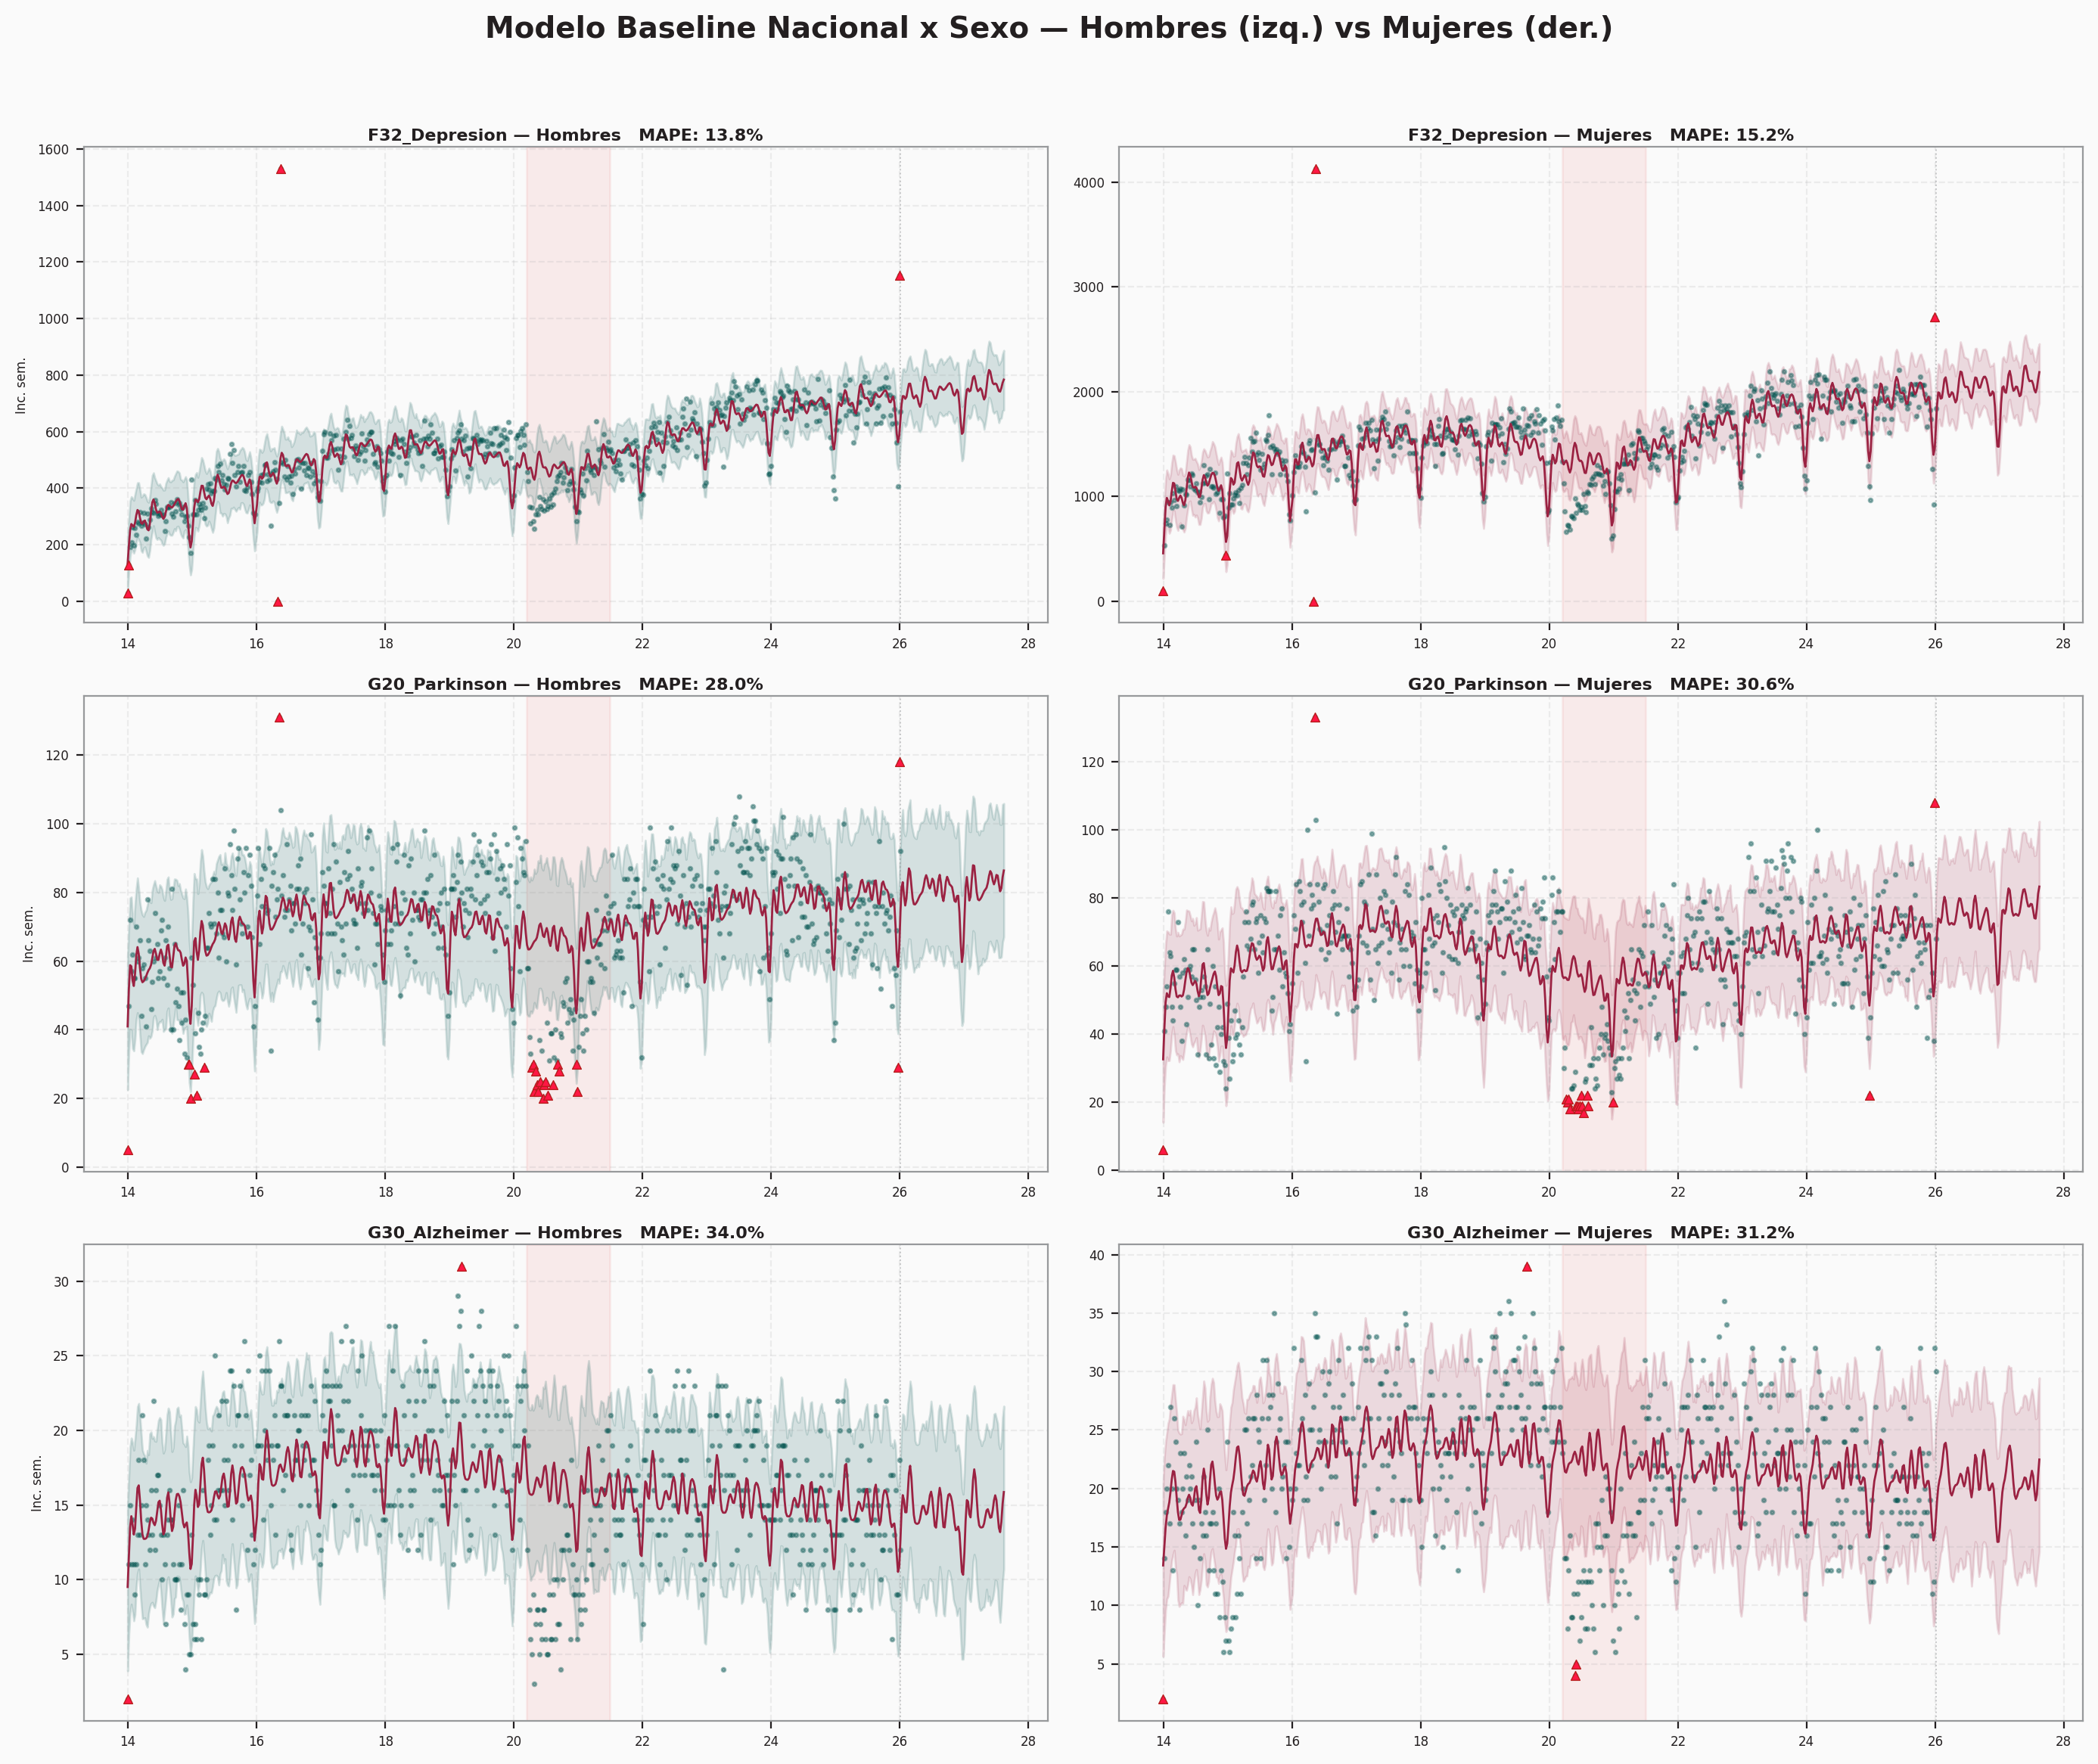
\includegraphics[width=\textwidth]{fig_15_sec13_2_nacional_sexo.png}
\caption{Comparativa nacional por sexo para los tres padecimientos.}
\label{fig:nacional-sexo}
\end{figure}

\subsection{Rankings Estatales}\label{sec:rankings}

Antes de examinar los rankings numéricos, las Figuras~\ref{fig:cuadricula-f32}--\ref{fig:cuadricula-g30} presentan la cuadrícula completa de los 32~modelos estatales por padecimiento. Cada panel muestra la serie observada, el pronóstico Prophet y el intervalo de predicción; el color del título indica la categoría de desempeño según los umbrales de la Sección~\ref{sec:desempeno}.

\subsubsection{Cuadrícula Estatal — Depresión (F32)}

La Figura~\ref{fig:cuadricula-f32} revela un espectro amplio de predecibilidad. Ciudad de México (5\%) y Jalisco (14\%) presentan ajustes notablemente precisos con bandas de predicción estrechas, lo cual se explica por el alto volumen de consultas y la estabilidad de sus sistemas de reporte. En contraste, estados como Guerrero (77\%), Puebla (73\%) y Coahuila (66\%) muestran pronósticos con bandas amplias y desfases sistemáticos, particularmente en el período post-COVID donde la recuperación del reporte sigue trayectorias irregulares. Se observa que los estados del sureste (Chiapas, Campeche, Quintana Roo) comparten un patrón de subestimación durante 2024--2025, sugiriendo un incremento regional en la incidencia de depresión que el modelo baseline no logra capturar completamente con los parámetros por defecto.

\begin{figure}[H]
\centering
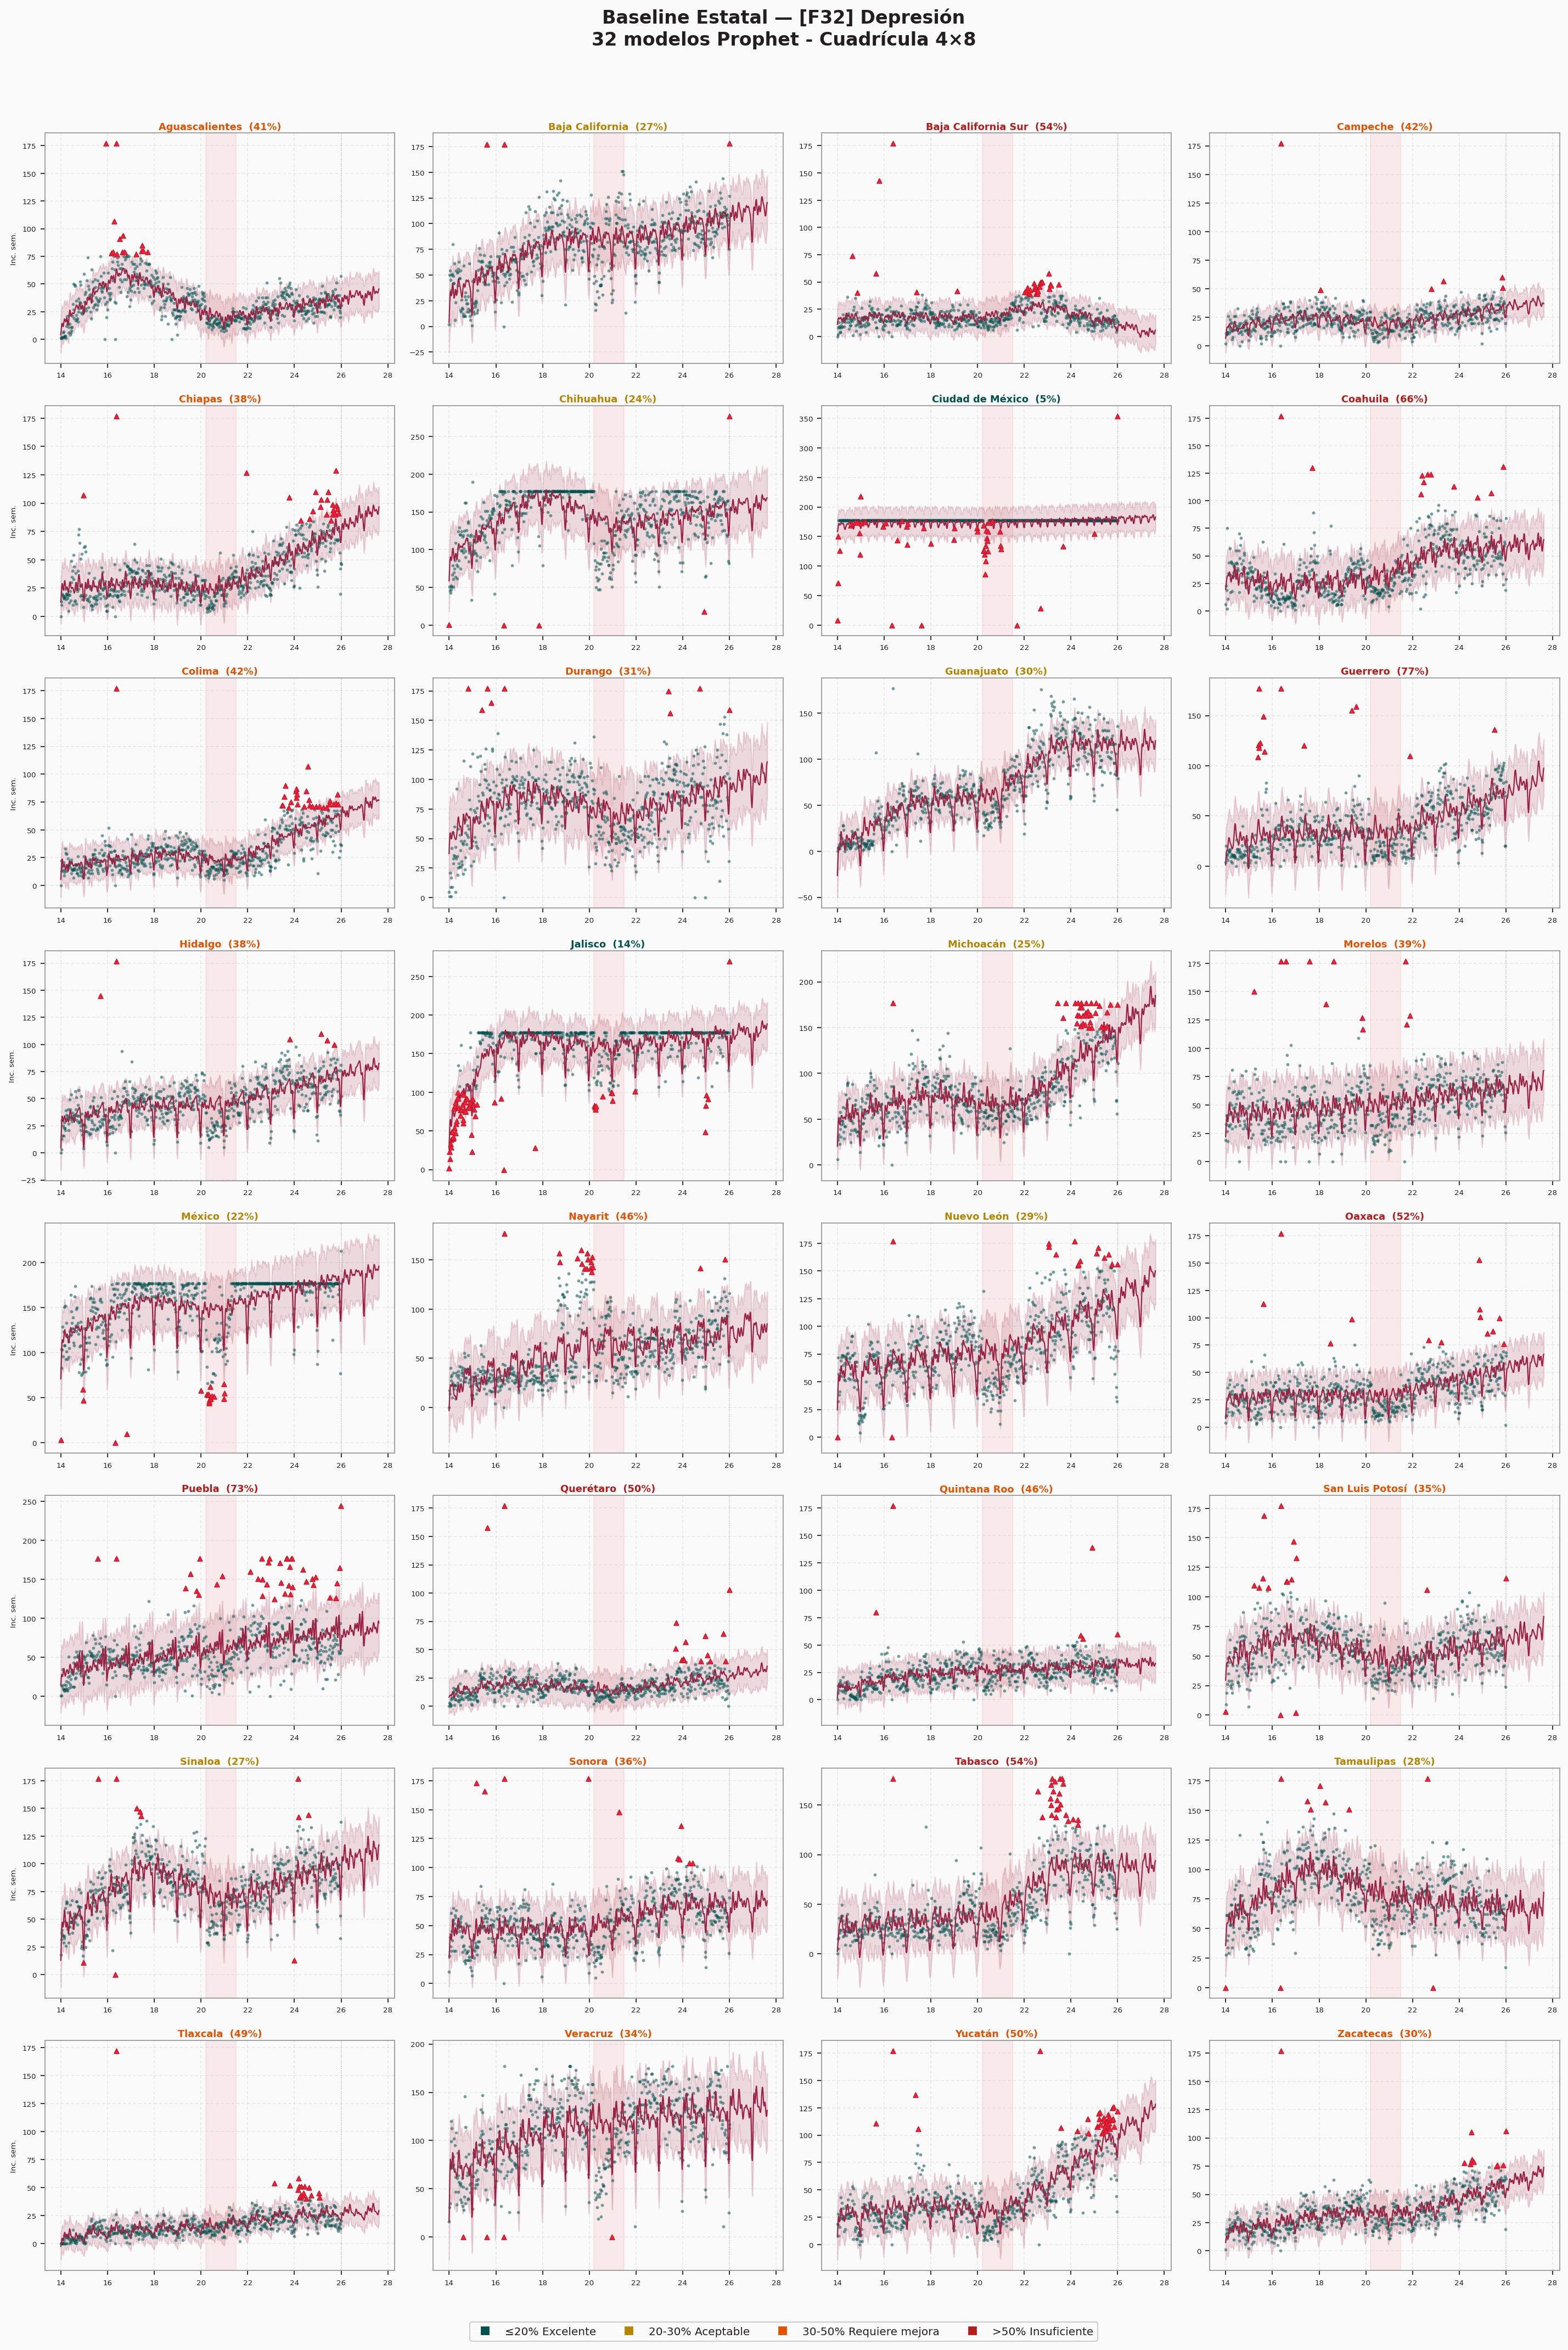
\includegraphics[width=\textwidth]{fig_19_sec13_3_cuadricula_F32_Depresion.png}
\caption{Cuadrícula de 32 modelos estatales — Depresión (F32). El color del título indica la categoría de desempeño: verde ($\leq$20\%), amarillo (20--30\%), naranja (30--50\%) y rojo ($>$50\%).}
\label{fig:cuadricula-f32}
\end{figure}

\subsubsection{Cuadrícula Estatal — Parkinson (G20)}

La cuadrícula de Parkinson (Figura~\ref{fig:cuadricula-g20}) evidencia el escenario más desafiante de los tres padecimientos. La totalidad de los estados presenta títulos en tonos naranjas y rojos, confirmando que 27 de 32 entidades se clasifican como \emph{Insuficientes}. Las series muestran un patrón característico de bajo volumen y alta volatilidad: los valores oscilan entre 0 y 12 casos semanales por 100,000~habitantes, generando una relación señal-ruido desfavorable para el modelo. Jalisco (36\%) destaca como la única entidad con un ajuste razonablemente aceptable, probablemente por su infraestructura hospitalaria de tercer nivel. Se observan bandas de predicción desproporcionadamente anchas en Durango (102\%) y Puebla (102\%), donde los intervalos cubren rangos negativos — un artefacto del modelo que subraya la necesidad de restricciones de no-negatividad en el Avance~4.

\begin{figure}[H]
\centering
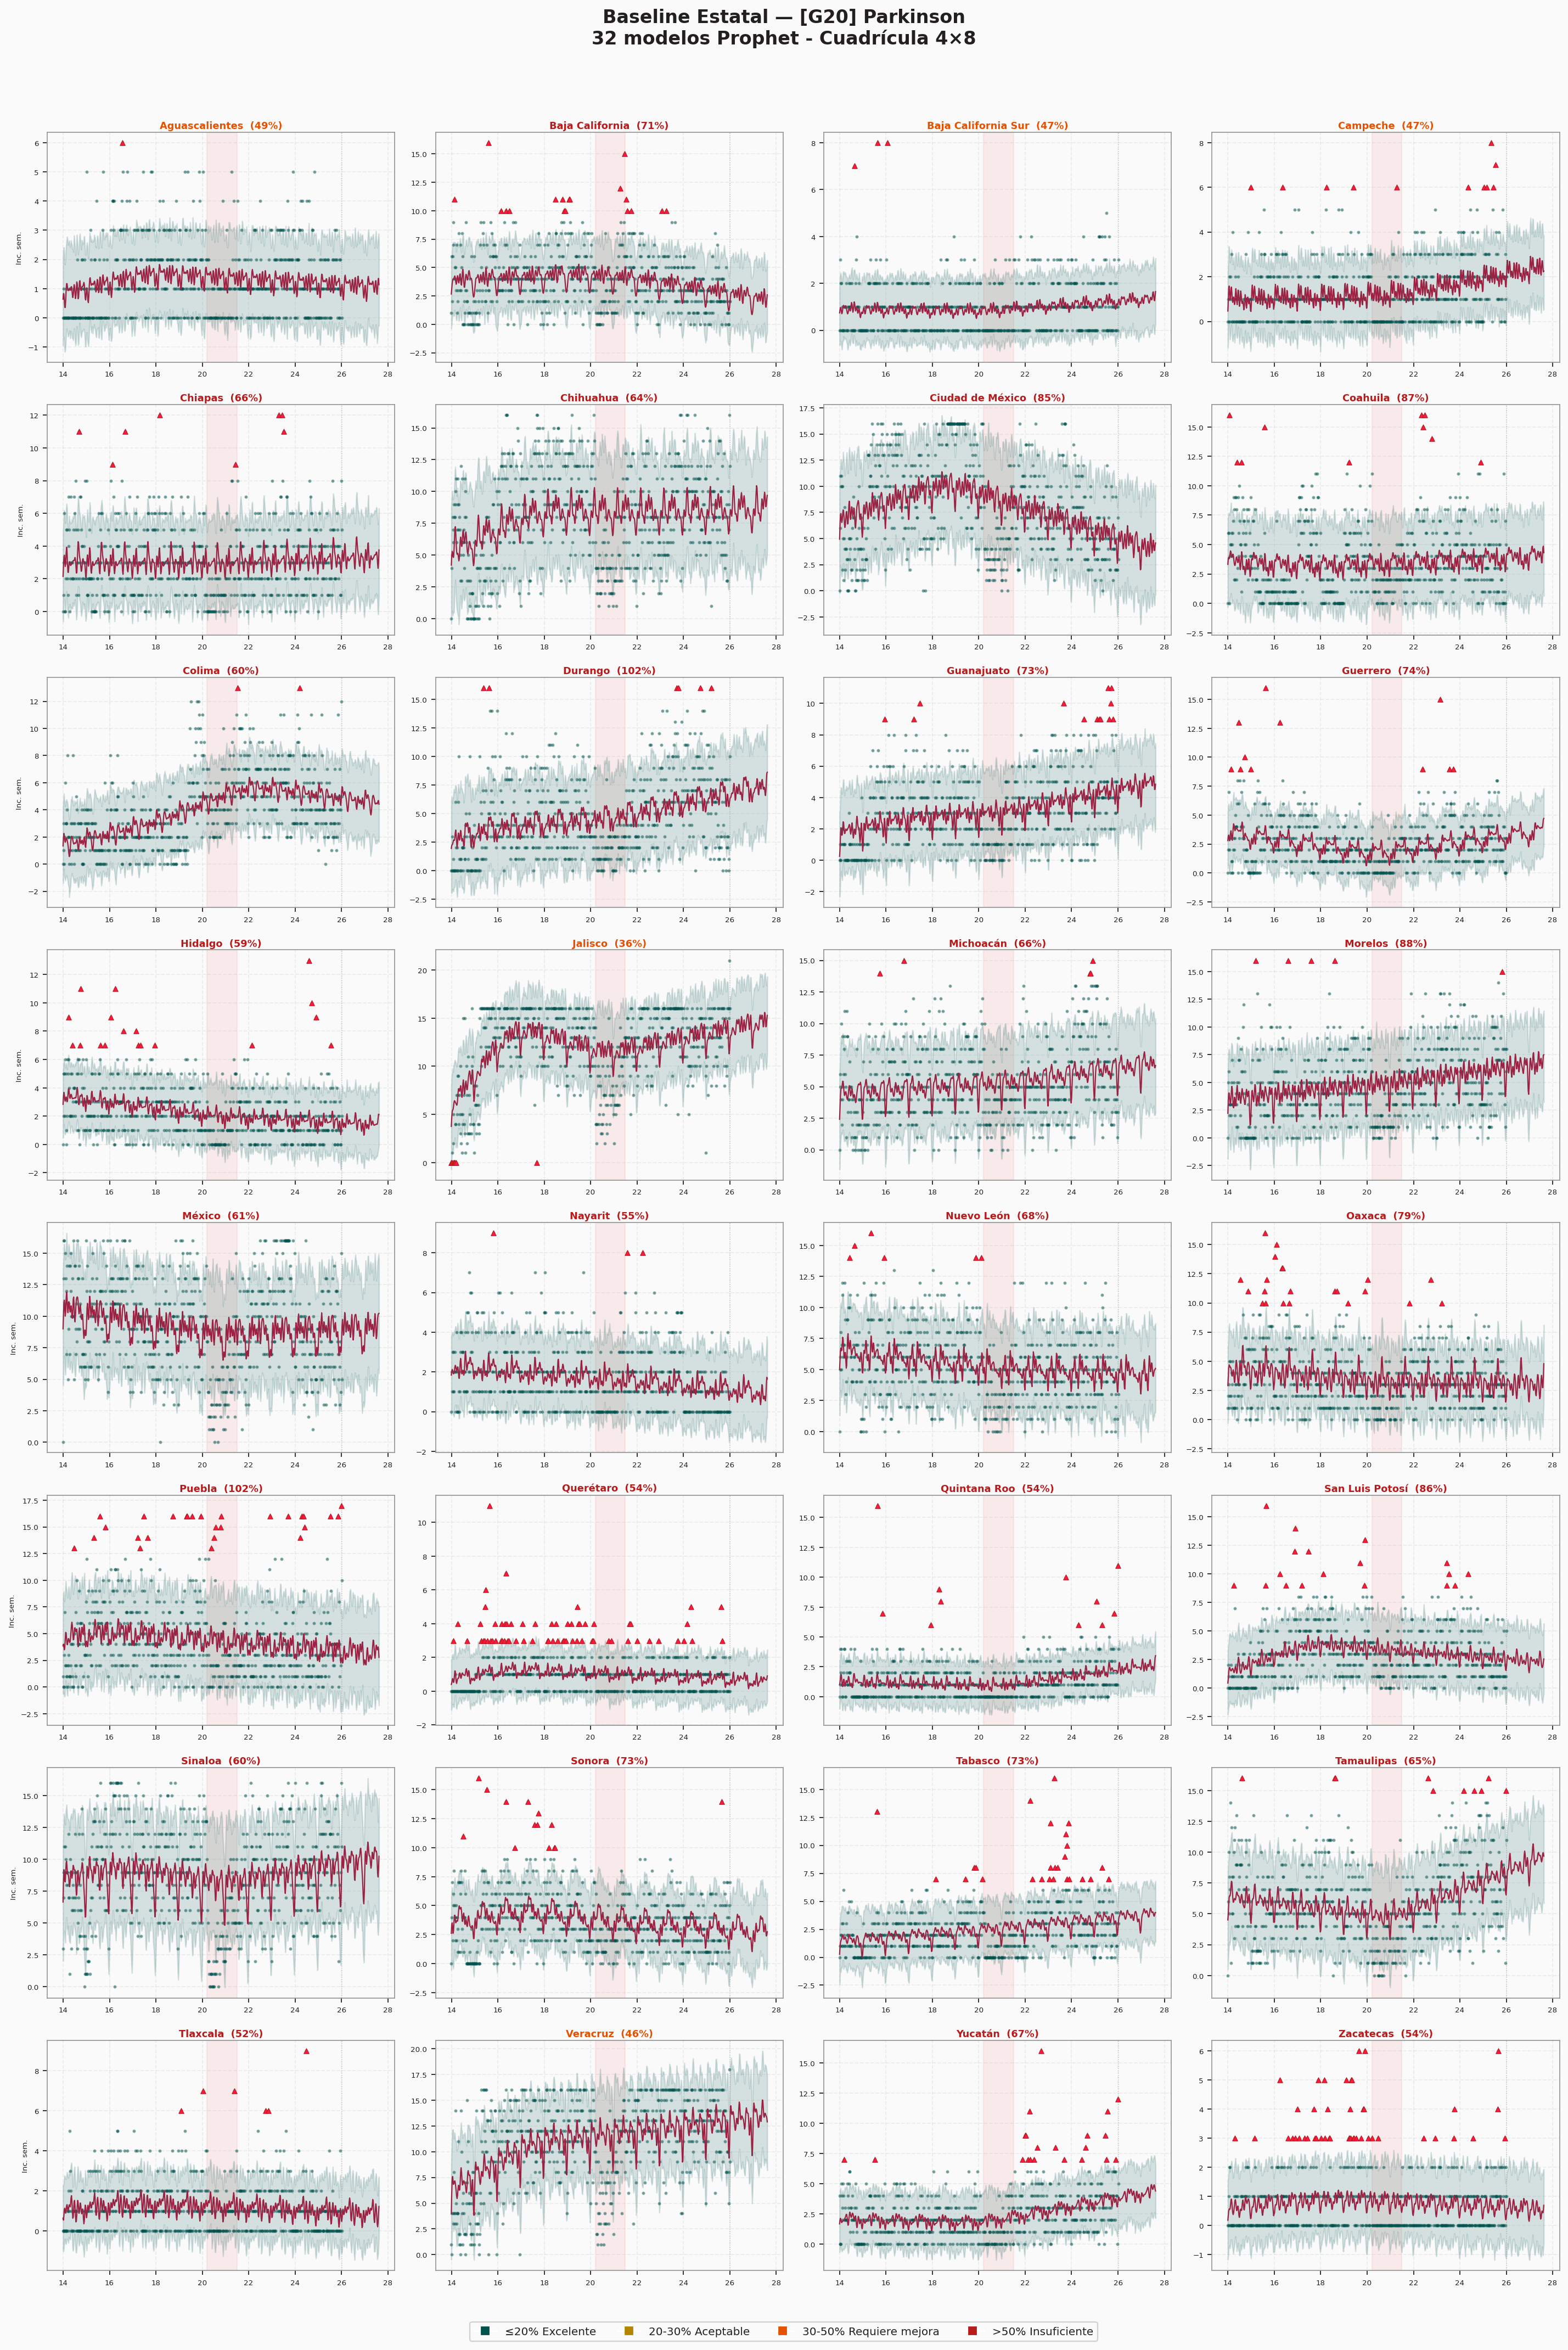
\includegraphics[width=\textwidth]{fig_20_sec13_3_cuadricula_G20_Parkinson.png}
\caption{Cuadrícula de 32 modelos estatales — Parkinson (G20). Nótense las bandas de predicción amplias y la predominancia de clasificaciones \emph{Insuficiente} (rojo) y \emph{Requiere mejora} (naranja).}
\label{fig:cuadricula-g20}
\end{figure}

\subsubsection{Cuadrícula Estatal — Alzheimer (G30)}

Alzheimer (Figura~\ref{fig:cuadricula-g30}) se ubica en una posición intermedia. Las series presentan volúmenes de incidencia aún menores que Parkinson (0--4 casos semanales por 100,000~habitantes), pero con un comportamiento más estable y estacional que facilita parcialmente el modelado. La mayoría de los estados se clasifica como \emph{Requiere mejora} (21 de 32), lo cual indica que los patrones temporales son detectables pero insuficientemente capturados por los hiperparámetros por defecto. Los estados con mejor desempeño — San Luis Potosí (39\%), Chiapas (40\%) y Tabasco (41\%) — comparten la característica de presentar series con tendencia plana y estacionalidad regular. En el extremo opuesto, Baja California Sur (75\%) muestra una serie con quiebres abruptos que el modelo no logra seguir, posiblemente vinculados a cambios en los protocolos de diagnóstico locales.

\begin{figure}[H]
\centering
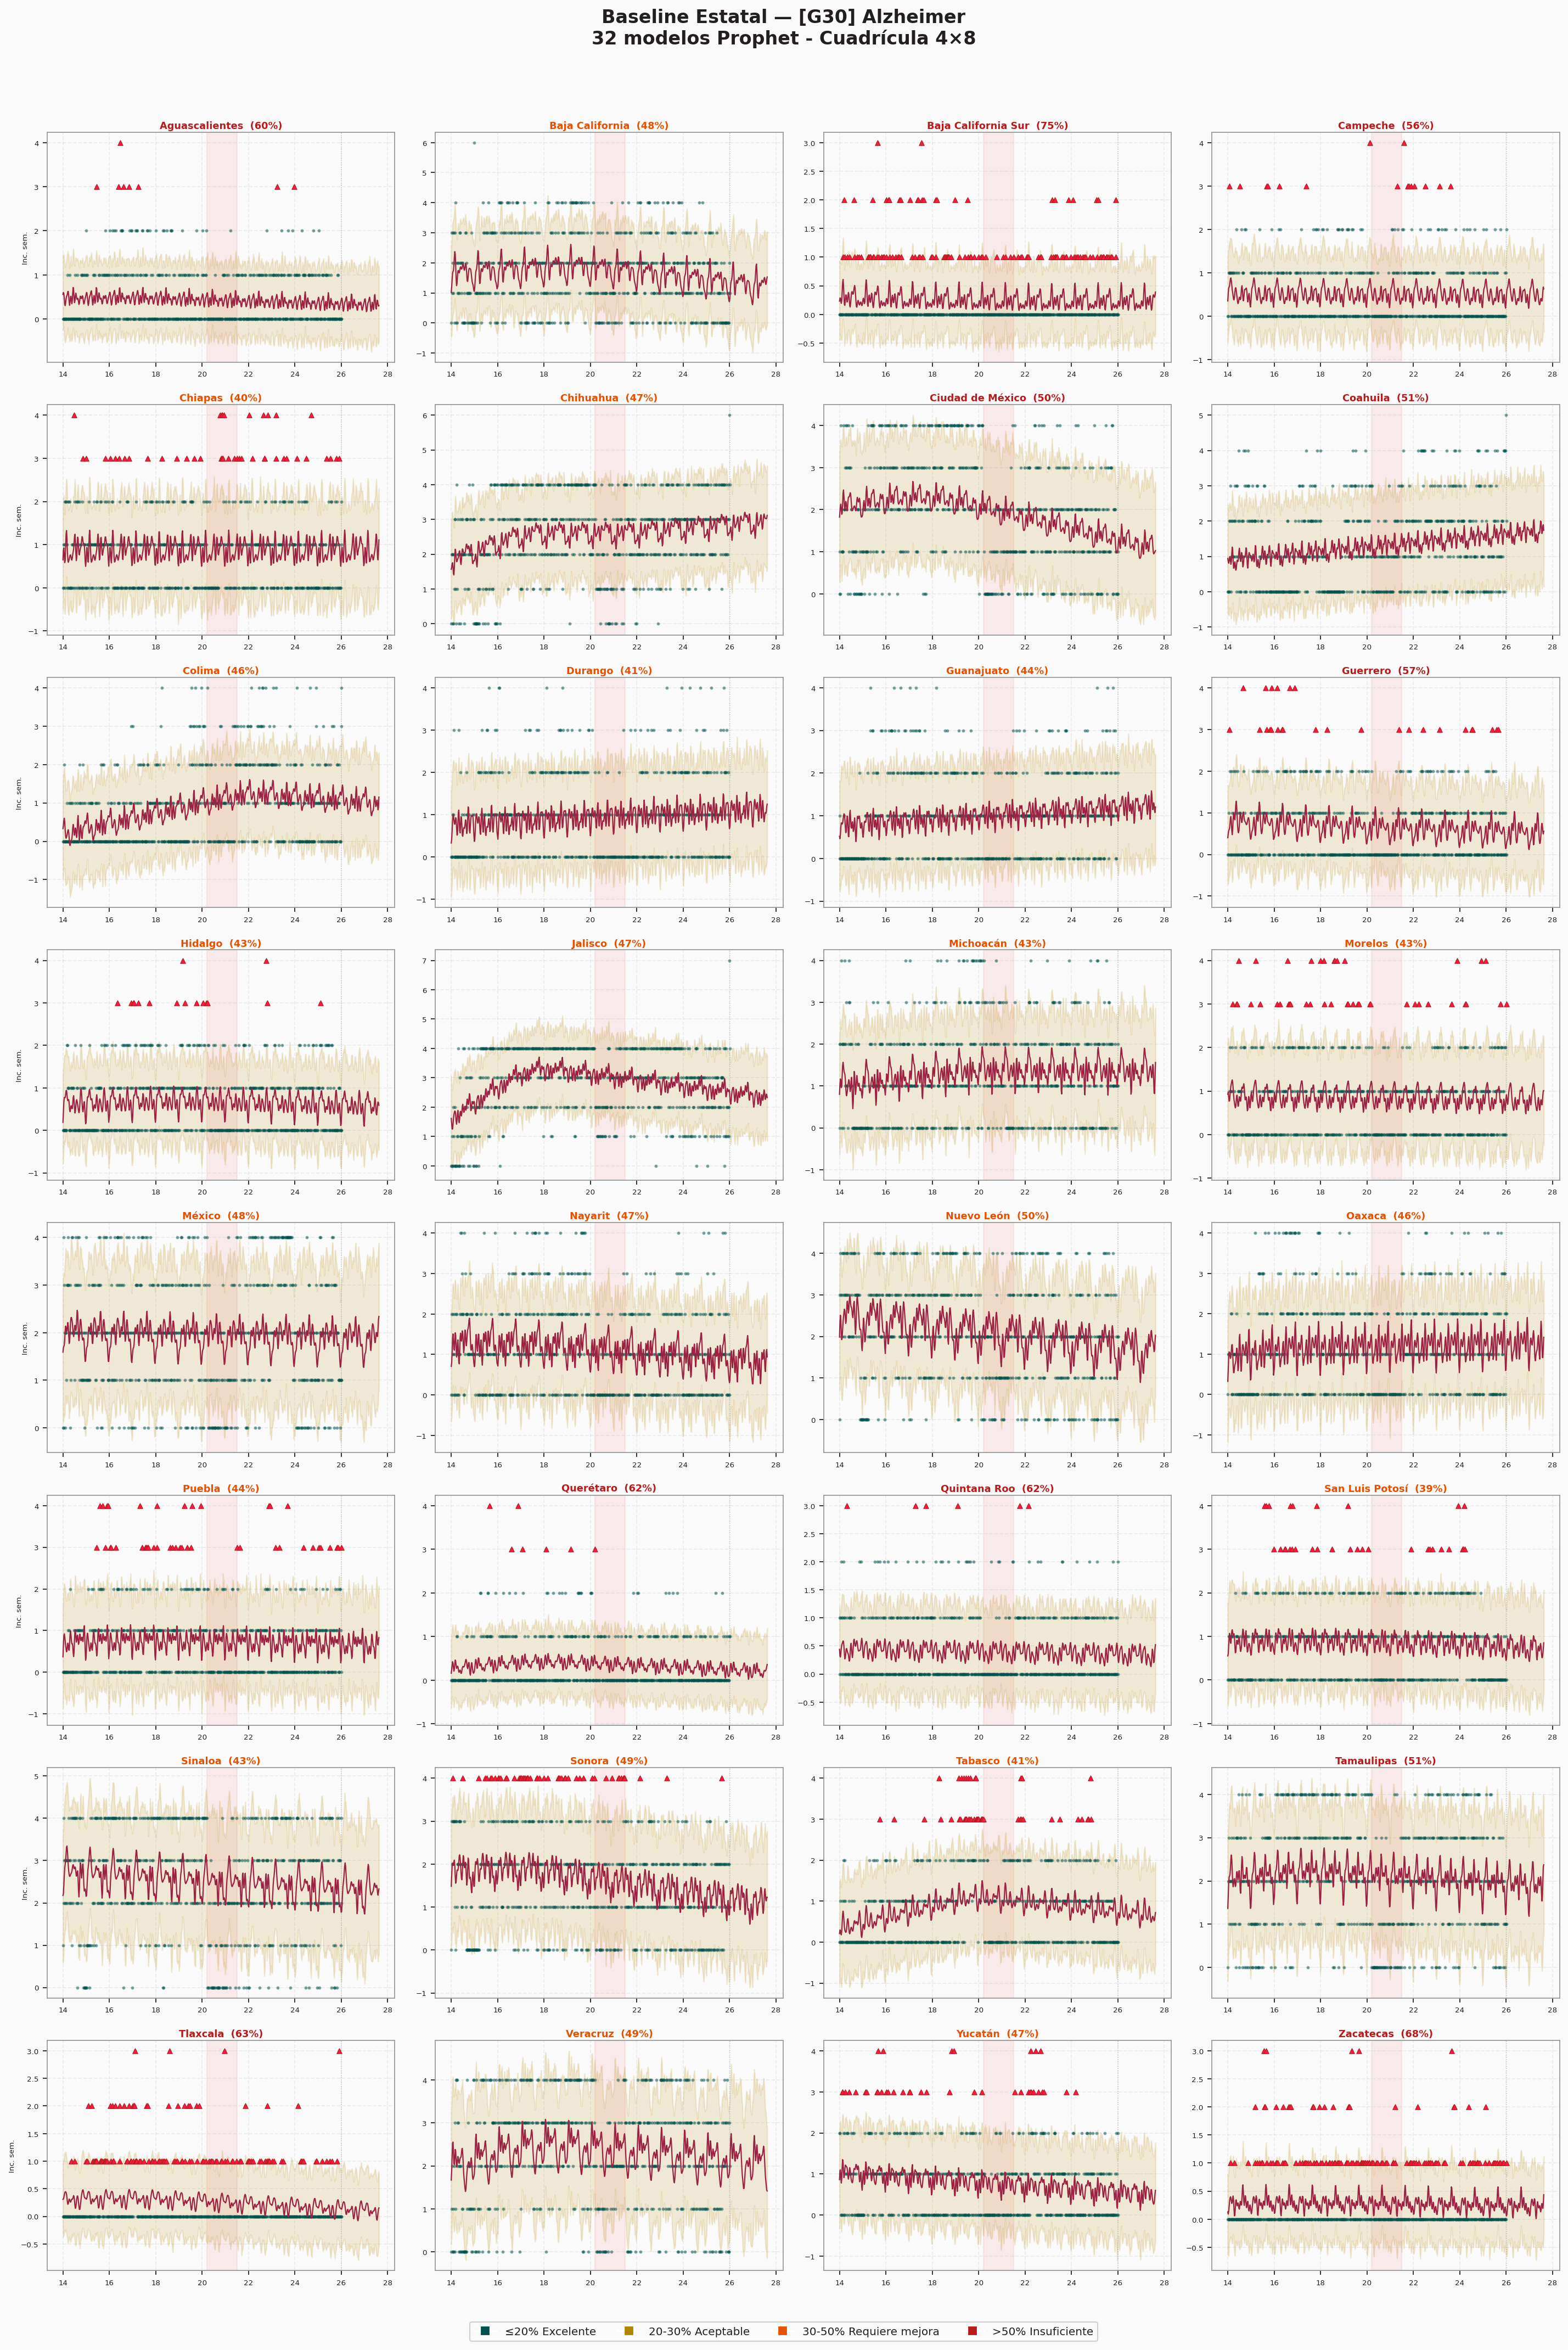
\includegraphics[width=\textwidth]{fig_21_sec13_3_cuadricula_G30_Alzheimer.png}
\caption{Cuadrícula de 32 modelos estatales — Alzheimer (G30). La clasificación predominante es \emph{Requiere mejora} (naranja), con una menor dispersión inter-estatal que Depresión.}
\label{fig:cuadricula-g30}
\end{figure}

La comparación visual entre las tres cuadrículas permite identificar un patrón transversal: los estados con infraestructura de vigilancia epidemiológica más robusta (Ciudad de México, Jalisco, Estado de México) tienden a presentar series más predecibles independientemente del padecimiento, mientras que entidades con sistemas de captura menos consolidados generan series ruidosas que degradan el desempeño de cualquier modelo estadístico. Esta observación refuerza la recomendación de la Dra.\ Grettel de evaluar la incorporación de indicadores de calidad de captura como variable exógena en el Avance~4.

La Tabla~\ref{tab:top5} y la Tabla~\ref{tab:bottom5} cuantifican los cinco estados con mejor y peor desempeño por padecimiento, confirmando numéricamente los patrones observados en las cuadrículas.

\begin{table}[H]
\centering
\caption{Top~5 estados con mejor desempeño (menor MAPE) por padecimiento.}
\label{tab:top5}
\resizebox{\textwidth}{!}{%
\begin{tabular}{@{}c l r l r l r@{}}
\toprule
\textbf{Rank} & \multicolumn{2}{c}{\textbf{Depresión}} & \multicolumn{2}{c}{\textbf{Parkinson}} & \multicolumn{2}{c}{\textbf{Alzheimer}} \\
\cmidrule(lr){2-3} \cmidrule(lr){4-5} \cmidrule(lr){6-7}
 & \textbf{Estado} & \textbf{MAPE} & \textbf{Estado} & \textbf{MAPE} & \textbf{Estado} & \textbf{MAPE} \\
\midrule
1 & Cd.\ de México & 4.79 & Jalisco & 36.04 & San Luis Potosí & 38.69 \\
2 & Jalisco & 14.20 & Veracruz & 46.24 & Chiapas & 40.13 \\
3 & México & 22.27 & Campeche & 46.56 & Tabasco & 40.92 \\
4 & Chihuahua & 24.21 & Baja Calif.\ Sur & 47.23 & Durango & 41.49 \\
5 & Michoacán & 25.10 & Aguascalientes & 48.82 & Hidalgo & 42.63 \\
\bottomrule
\end{tabular}%
}
\end{table}

\begin{table}[H]
\centering
\caption{Bottom~5 estados con peor desempeño (mayor MAPE) por padecimiento.}
\label{tab:bottom5}
\resizebox{\textwidth}{!}{%
\begin{tabular}{@{}c l r l r l r@{}}
\toprule
\textbf{Rank} & \multicolumn{2}{c}{\textbf{Depresión}} & \multicolumn{2}{c}{\textbf{Parkinson}} & \multicolumn{2}{c}{\textbf{Alzheimer}} \\
\cmidrule(lr){2-3} \cmidrule(lr){4-5} \cmidrule(lr){6-7}
 & \textbf{Estado} & \textbf{MAPE} & \textbf{Estado} & \textbf{MAPE} & \textbf{Estado} & \textbf{MAPE} \\
\midrule
1 & Guerrero & 77.43 & Puebla & 102.27 & Baja Calif.\ Sur & 74.74 \\
2 & Puebla & 72.92 & Durango & 101.63 & Zacatecas & 67.56 \\
3 & Coahuila & 66.16 & Morelos & 87.73 & Tlaxcala & 63.27 \\
4 & Tabasco & 54.49 & Coahuila & 86.67 & Quintana Roo & 62.43 \\
5 & Baja Calif.\ Sur & 53.64 & San Luis Potosí & 86.31 & Querétaro & 61.56 \\
\bottomrule
\end{tabular}%
}
\end{table}

Se observa una heterogeneidad notable: Ciudad de México alcanza un MAPE de apenas 4.79\% en Depresión, mientras que Puebla supera el 100\% en Parkinson, reflejando las diferencias en infraestructura de captura de datos entre entidades federativas.

\subsection{Heatmaps por Sexo}\label{sec:heatmaps-sexo}

Las Figuras~\ref{fig:heatmap-f32}--\ref{fig:heatmap-g30} presentan los heatmaps del MAPE estatal desagregado por sexo para cada padecimiento.

\begin{figure}[H]
\centering
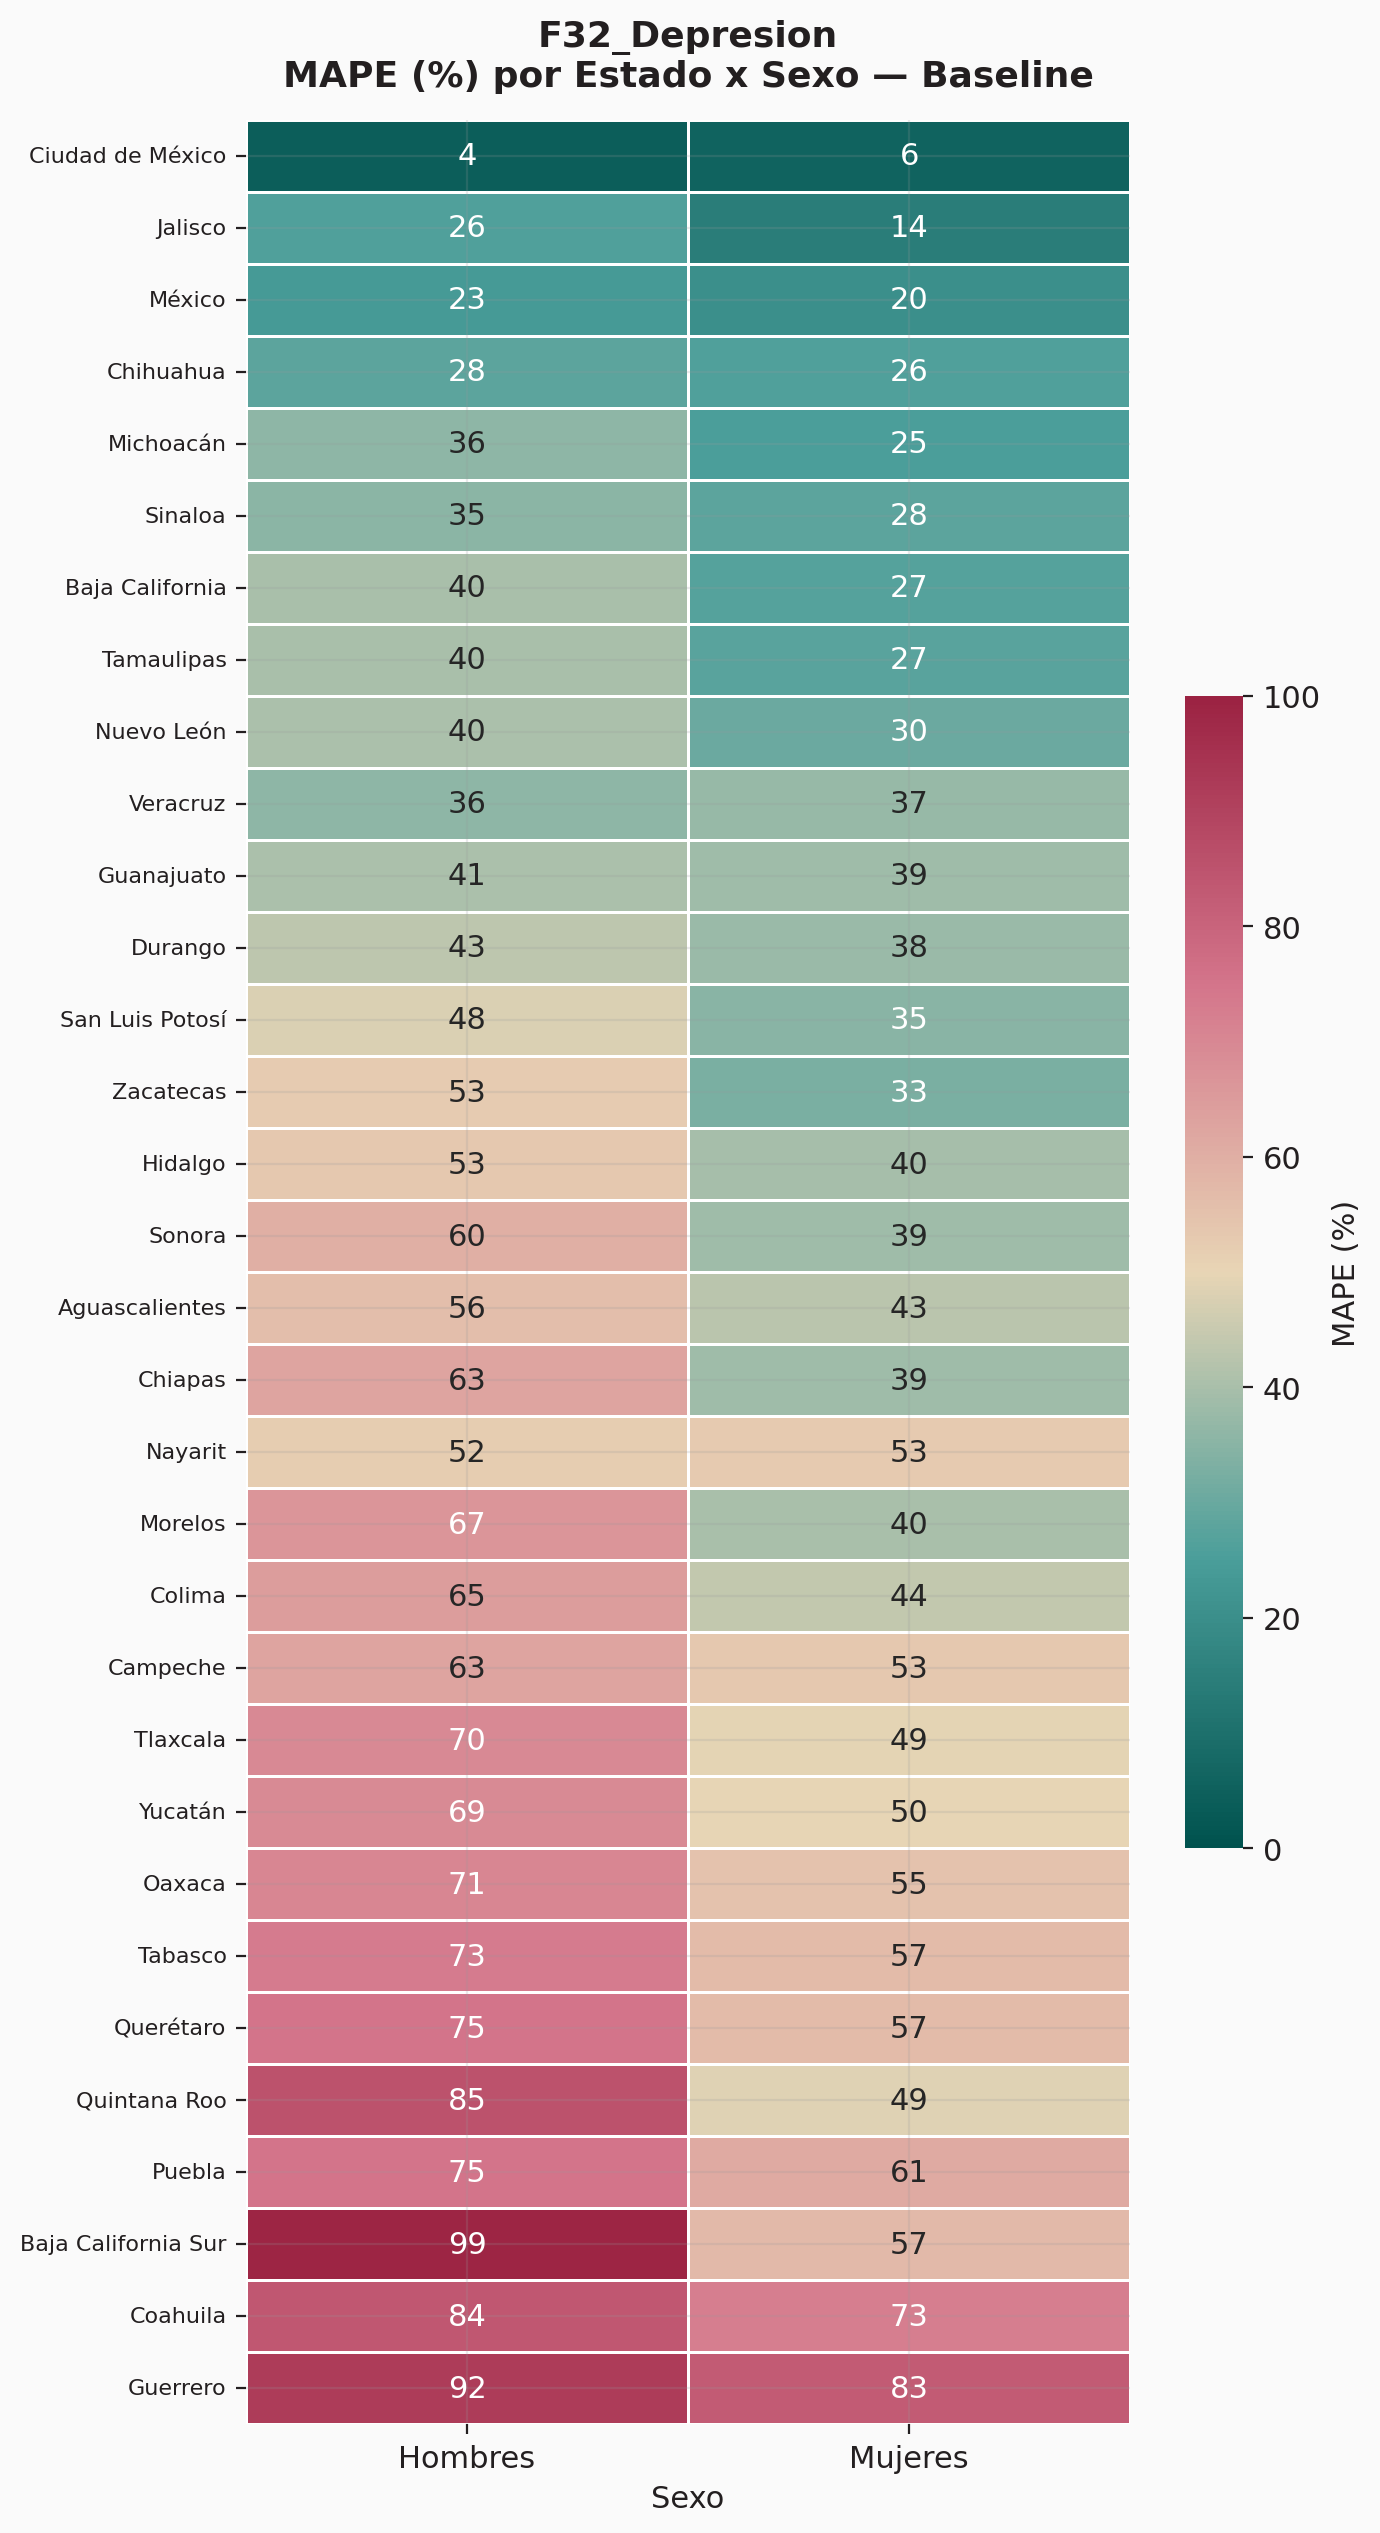
\includegraphics[width=0.85\textwidth]{fig_16_sec13_5_heatmap_sexo_F32_Depresion.png}
\caption{Heatmap MAPE por estado y sexo — Depresión (F32).}
\label{fig:heatmap-f32}
\end{figure}

\begin{figure}[H]
\centering
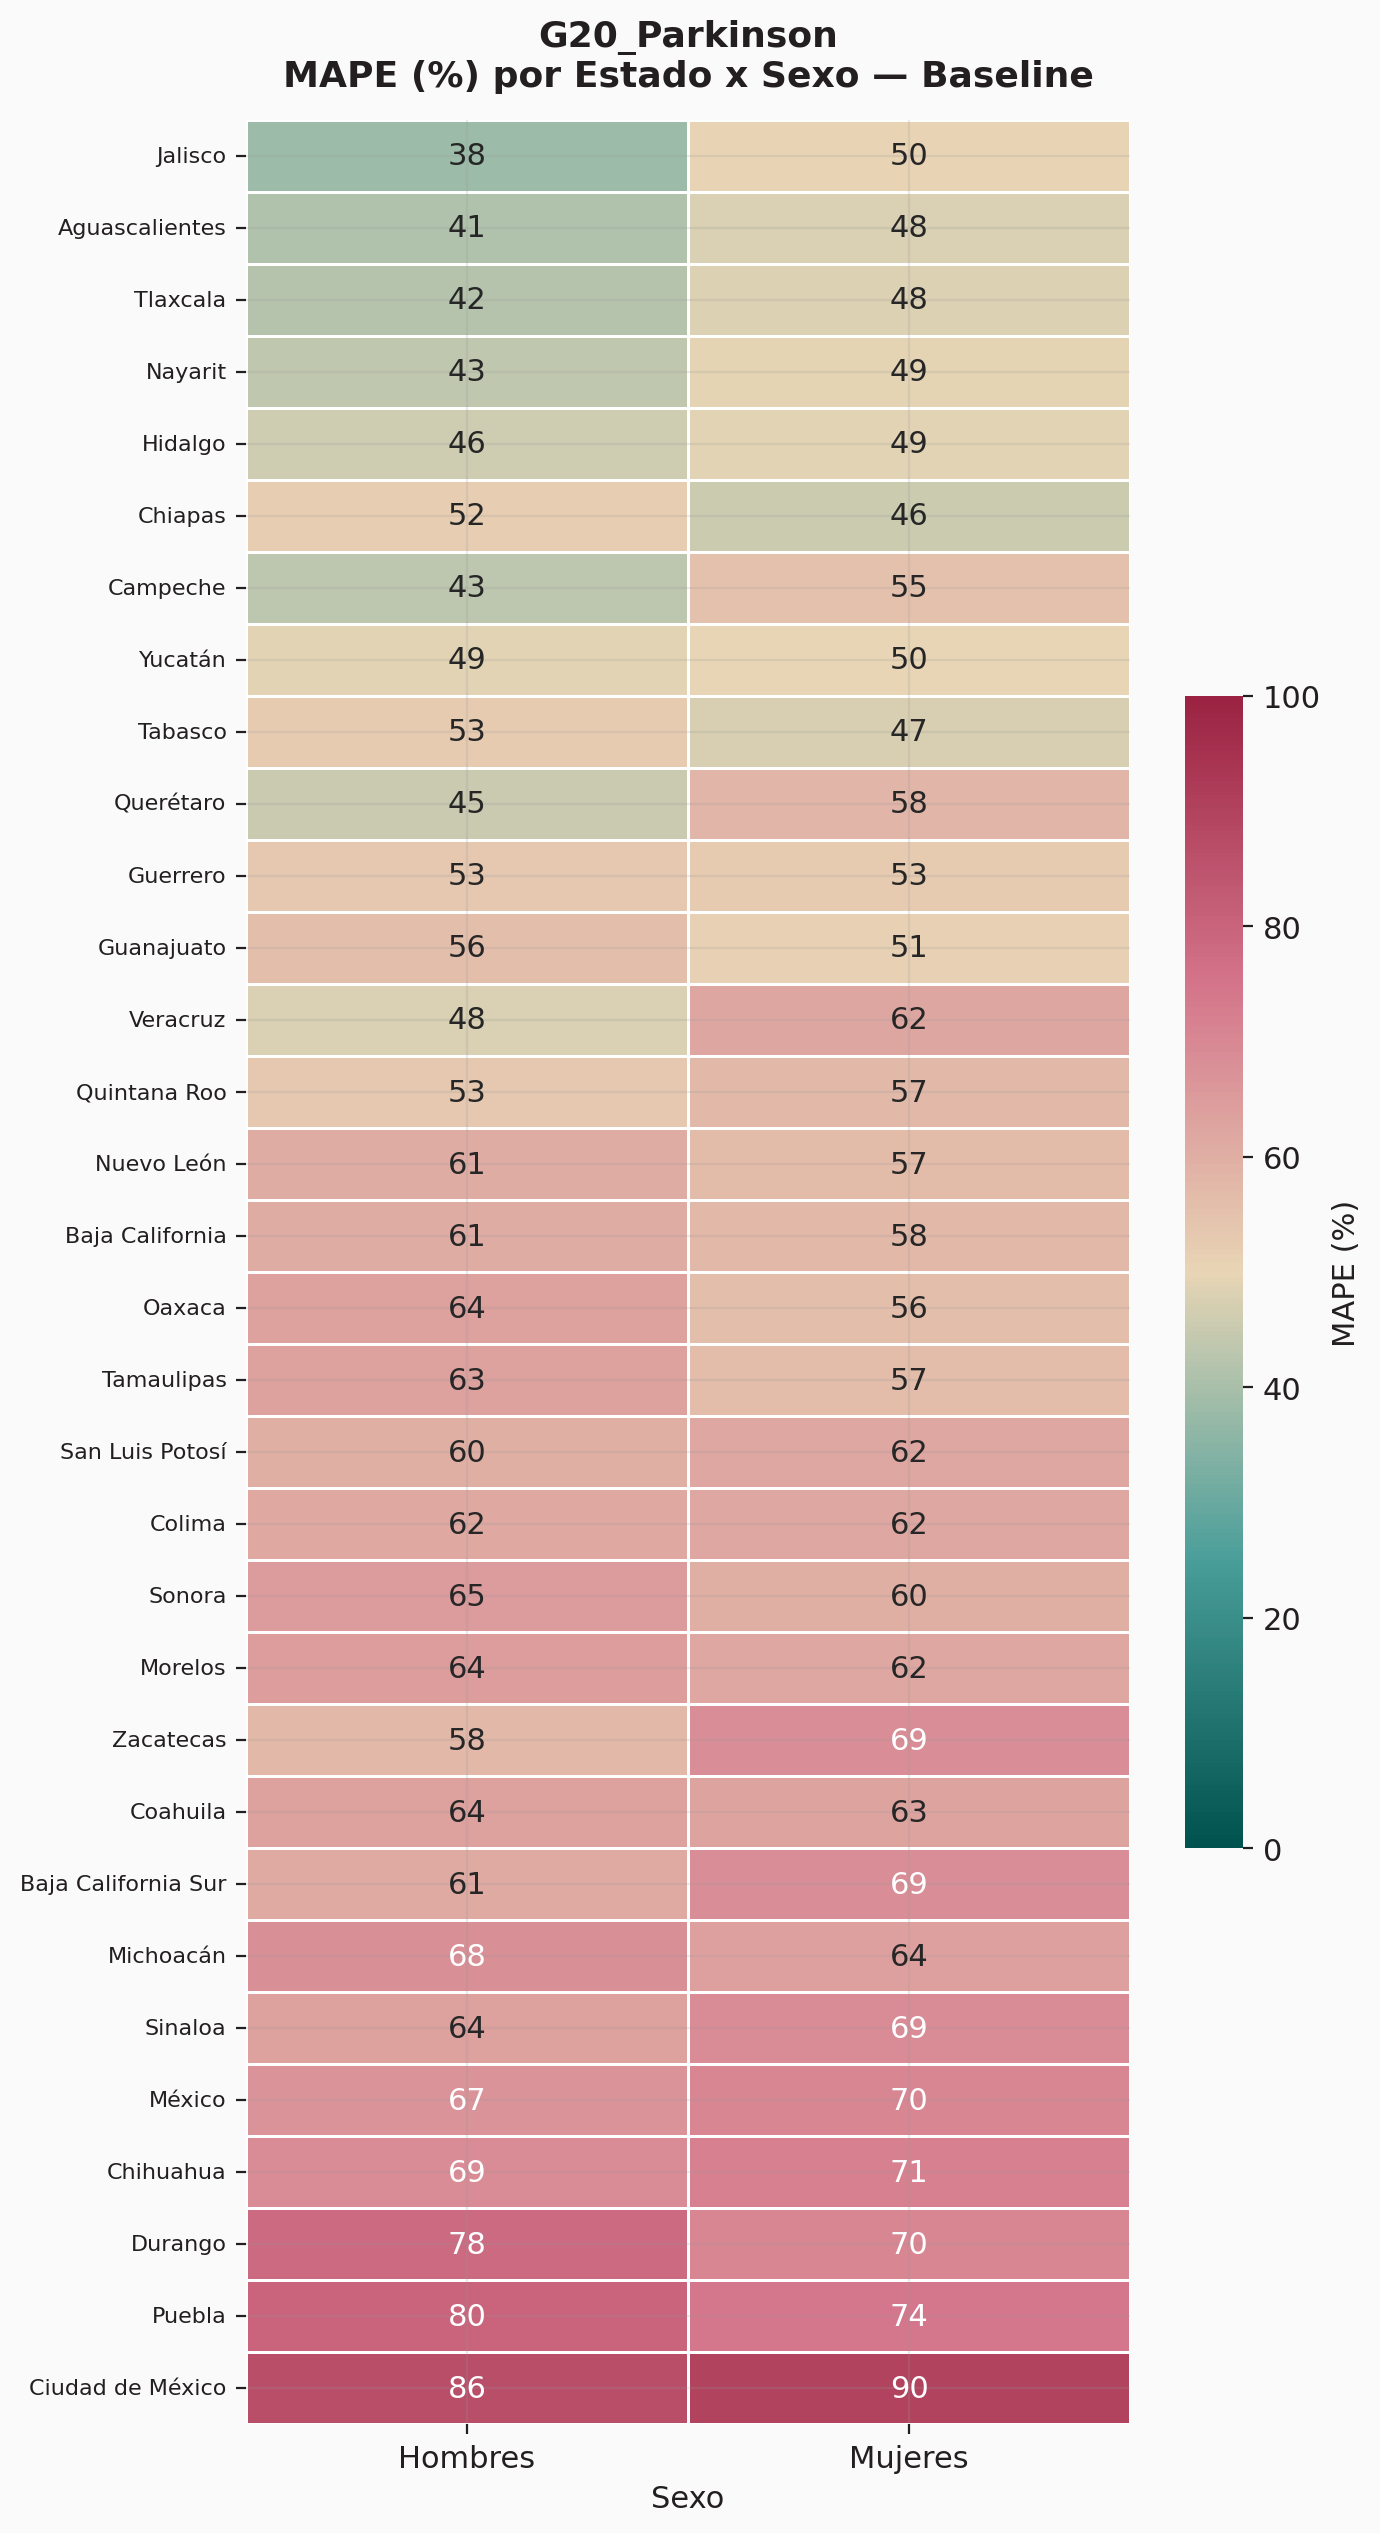
\includegraphics[width=0.85\textwidth]{fig_17_sec13_5_heatmap_sexo_G20_Parkinson.png}
\caption{Heatmap MAPE por estado y sexo — Parkinson (G20).}
\label{fig:heatmap-g20}
\end{figure}

\begin{figure}[H]
\centering
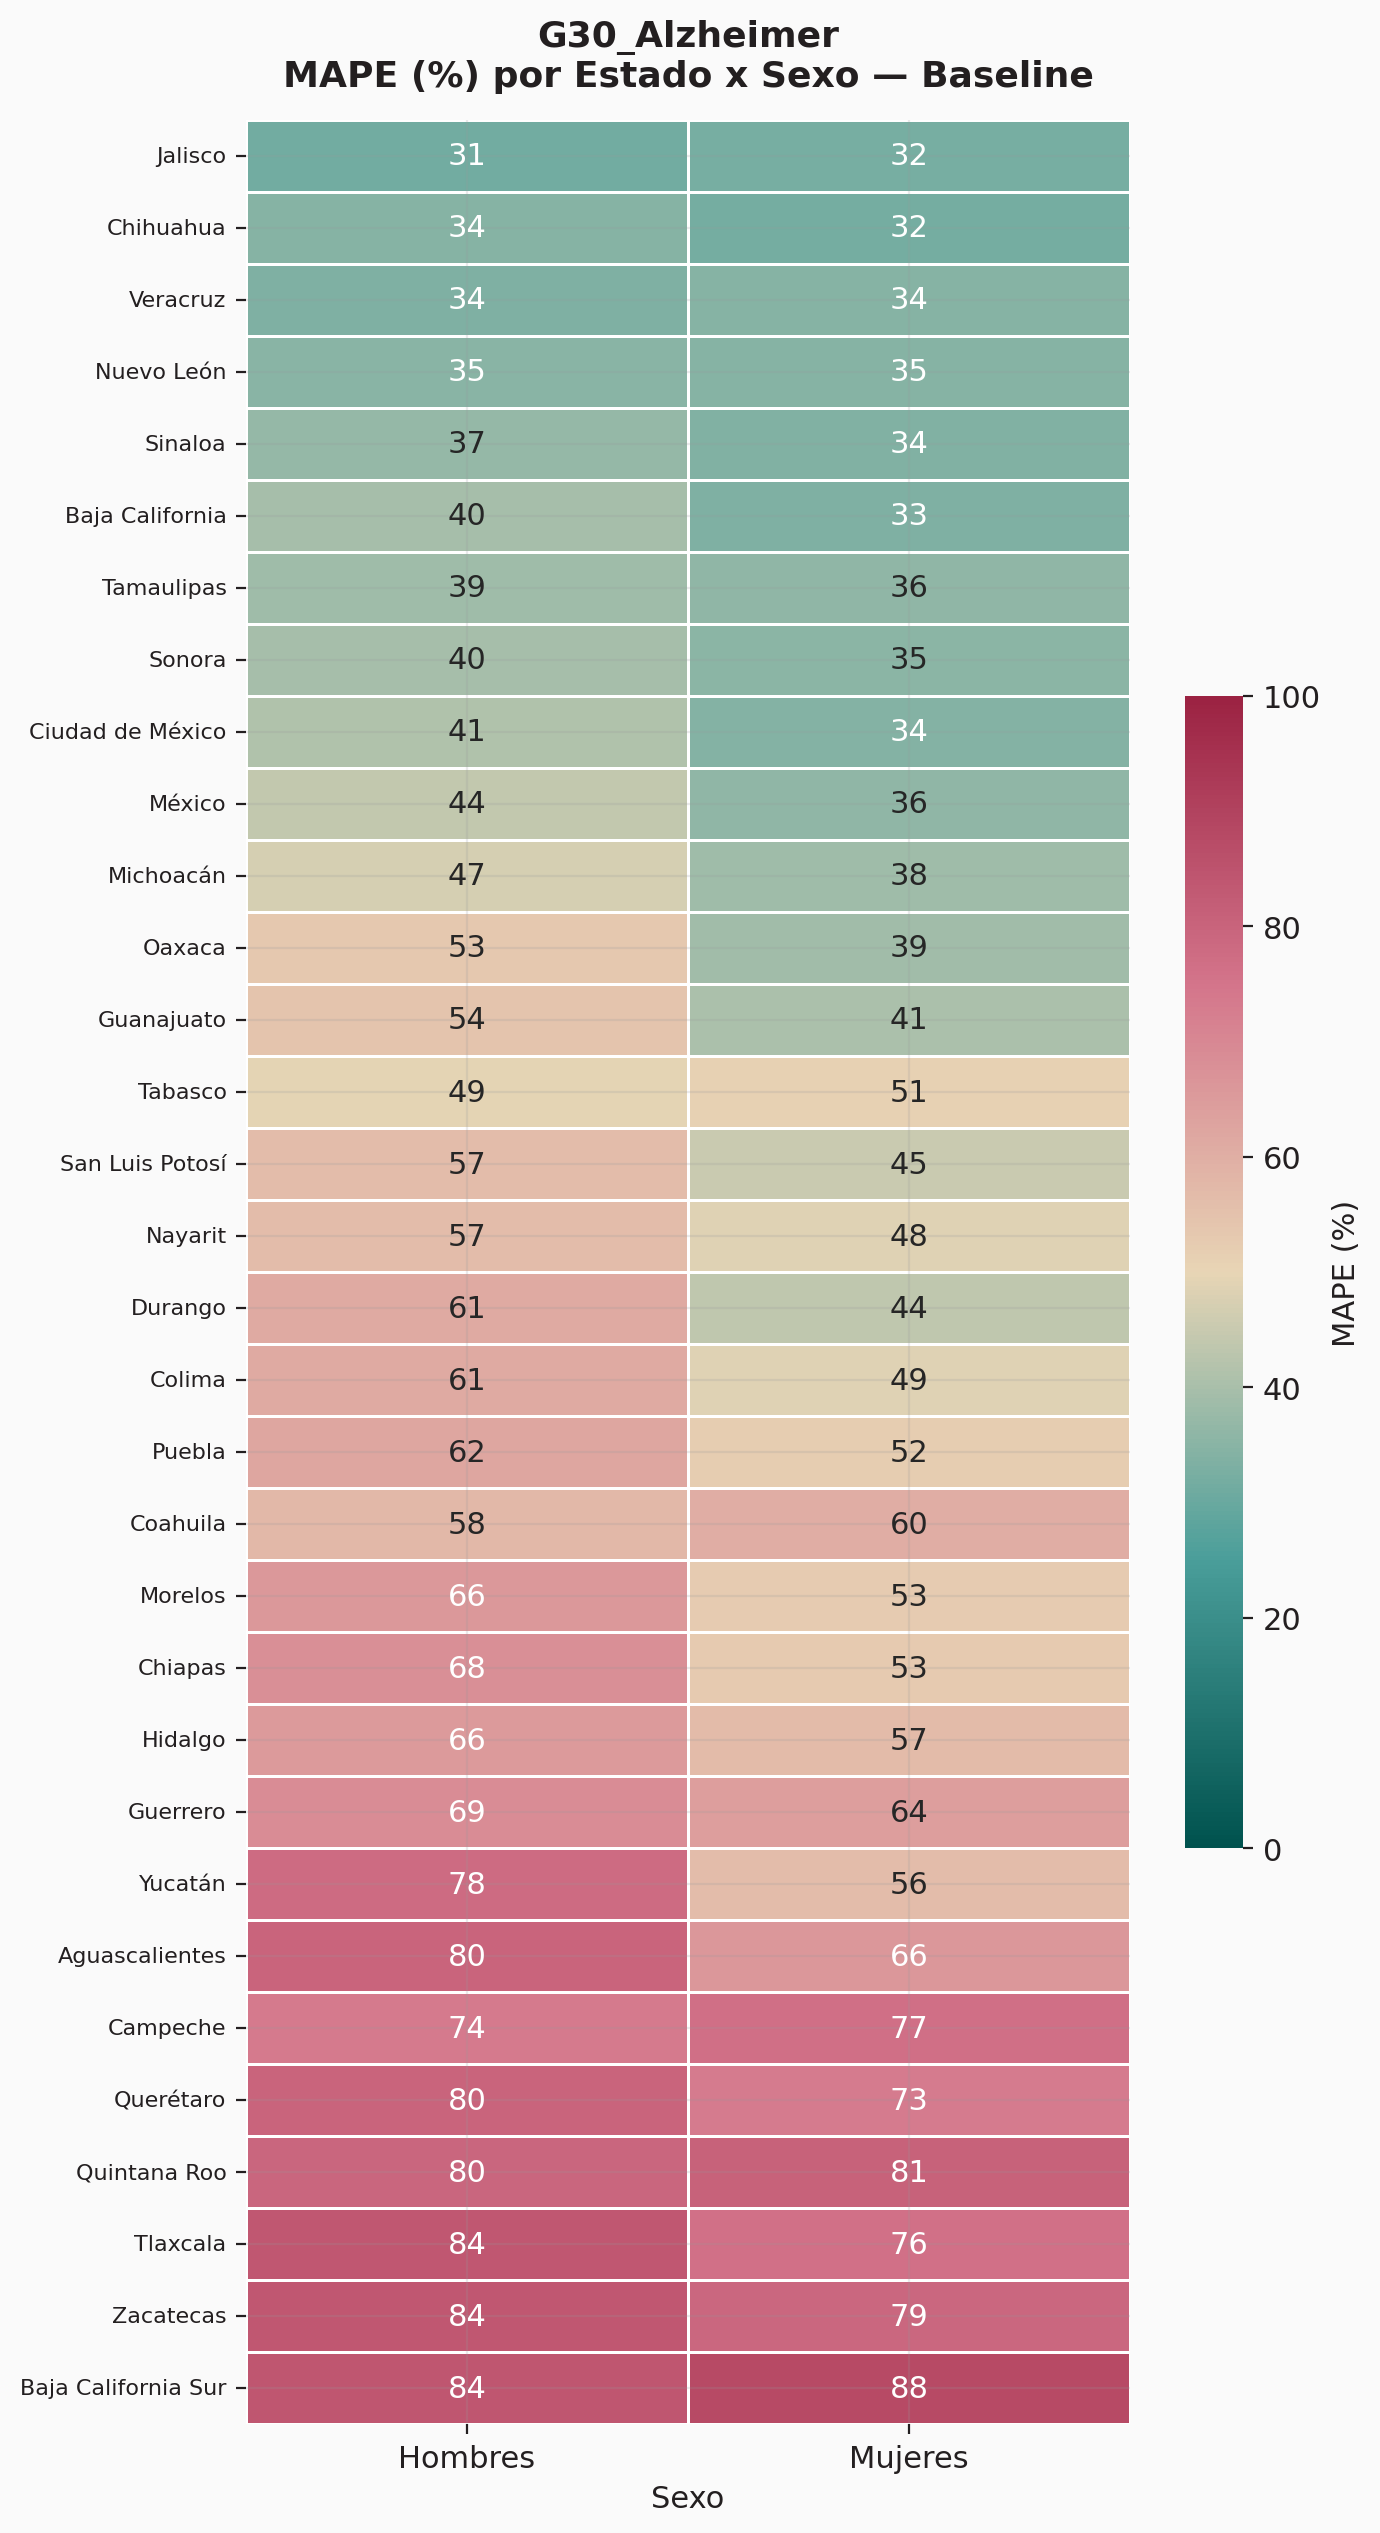
\includegraphics[width=0.85\textwidth]{fig_18_sec13_5_heatmap_sexo_G30_Alzheimer.png}
\caption{Heatmap MAPE por estado y sexo — Alzheimer (G30).}
\label{fig:heatmap-g30}
\end{figure}

\subsection{Dashboard Integral del Modelo Baseline}\label{sec:dashboard-integral}

La Figura~\ref{fig:dashboard-integral} consolida en un único panel los indicadores clave de los 297~modelos baseline. El dashboard se organiza en siete filas por padecimiento: (1)~tarjetas KPI con MAPE nacional, RMSE, mediana estatal y total de modelos; (2)~gráficos de dona con la distribución semáforo de las 32~entidades; (3)~rankings de los tres mejores y peores estados; (4)~barras horizontales con el ranking completo de MAPE por entidad; (5)~comparativa Hombres vs.\ Mujeres a nivel nacional; (6)~diagramas de dispersión Train vs.\ CV para diagnóstico de sub/sobreajuste; y (7)~resumen de calidad con outliers, volatilidad y brecha de generalización.

La lectura transversal del dashboard permite identificar con claridad las asimetrías entre padecimientos: Depresión concentra 10 de 32 estados en categorías \emph{Excelente} o \emph{Aceptable} (31.3\%), mientras que Parkinson no logra ubicar ningún estado por debajo del 30\% de MAPE. Alzheimer se sitúa en una posición intermedia con la menor dispersión inter-estatal (desviación estándar de 8.6\%) pero sin estados en las categorías superiores. La fila de sub/sobreajuste confirma que los tres padecimientos presentan puntos consistentemente por encima de la diagonal, indicando que la brecha Train--CV es generalizada y no producto de casos aislados.

\begin{figure}[H]
\centering
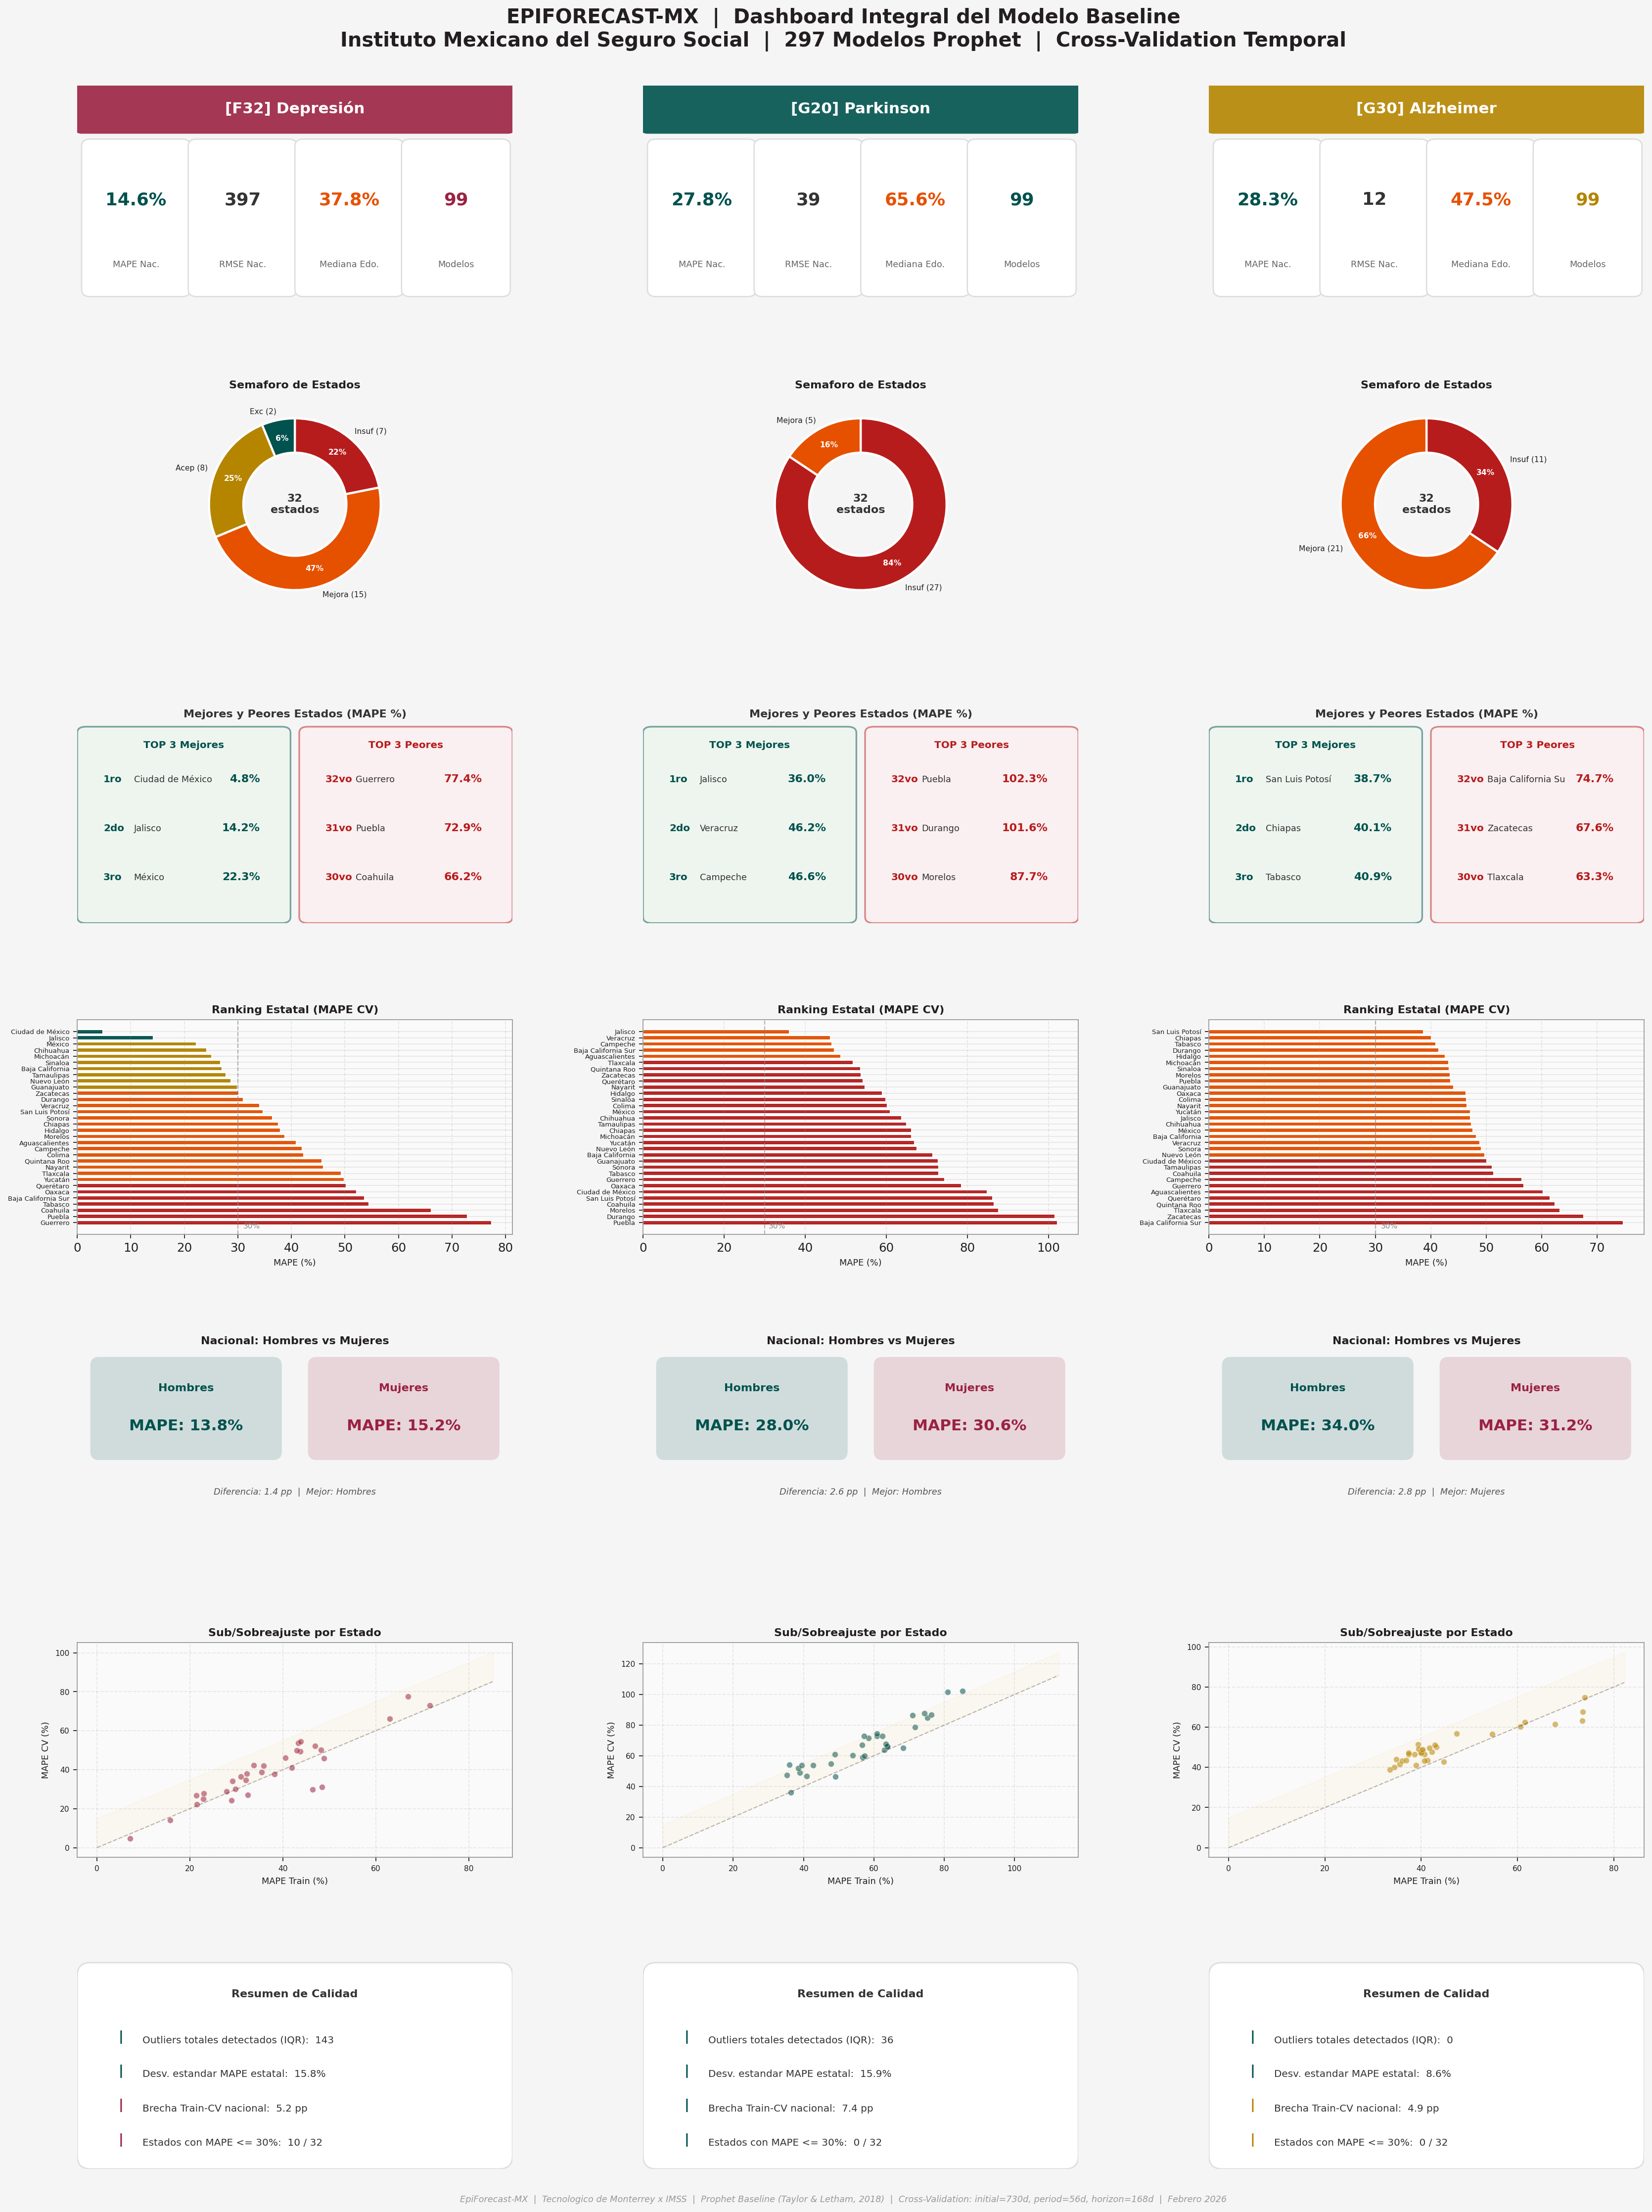
\includegraphics[width=\textwidth]{fig_22_sec13_7_dashboard_integral.png}
\caption{Dashboard integral del modelo baseline — EpiForecast-MX. Panorama comparativo de los tres padecimientos con KPIs, semáforo estatal, rankings, comparativa por sexo, diagnóstico de ajuste y resumen de calidad para los 297~modelos Prophet.}
\label{fig:dashboard-integral}
\end{figure}

% =============================================================================
%  9. DASHBOARD TABLEAU — DOCUMENTACIÓN TÉCNICA
% =============================================================================
\section{Dashboard Tableau — Documentación Técnica}\label{sec:tableau}

El dashboard interactivo en Tableau Public (\url{https://proyectointegrador.org/epidashboard}) fue actualizado con base en el \emph{feedback} recibido de la Dra.\ Ruth Pérez, la Dra.\ Lina Díaz Castro y la Dra.\ Grettel Barceló durante las reuniones de seguimiento semanales. Esta sección documenta las decisiones técnicas implementadas.

\subsection{Filtrado Dinámico y Ajustes de Usabilidad}\label{sec:tableau-filtros}

Se incorporó un filtro por entidad federativa que mantiene la opción ``All'' para alternar entre análisis nacional y estatal. El filtro de padecimiento fue configurado en modo de selección única, eliminando la opción de selección múltiple y la alternativa ``All'', dado que la agregación simultánea de padecimientos no tiene una interpretación epidemiológica válida y puede inducir lecturas erróneas. Se realizaron ajustes de estandarización en tipografías, tamaños de fuente y colores para homogeneizar la jerarquía visual.

\begin{figure}[H]
\centering
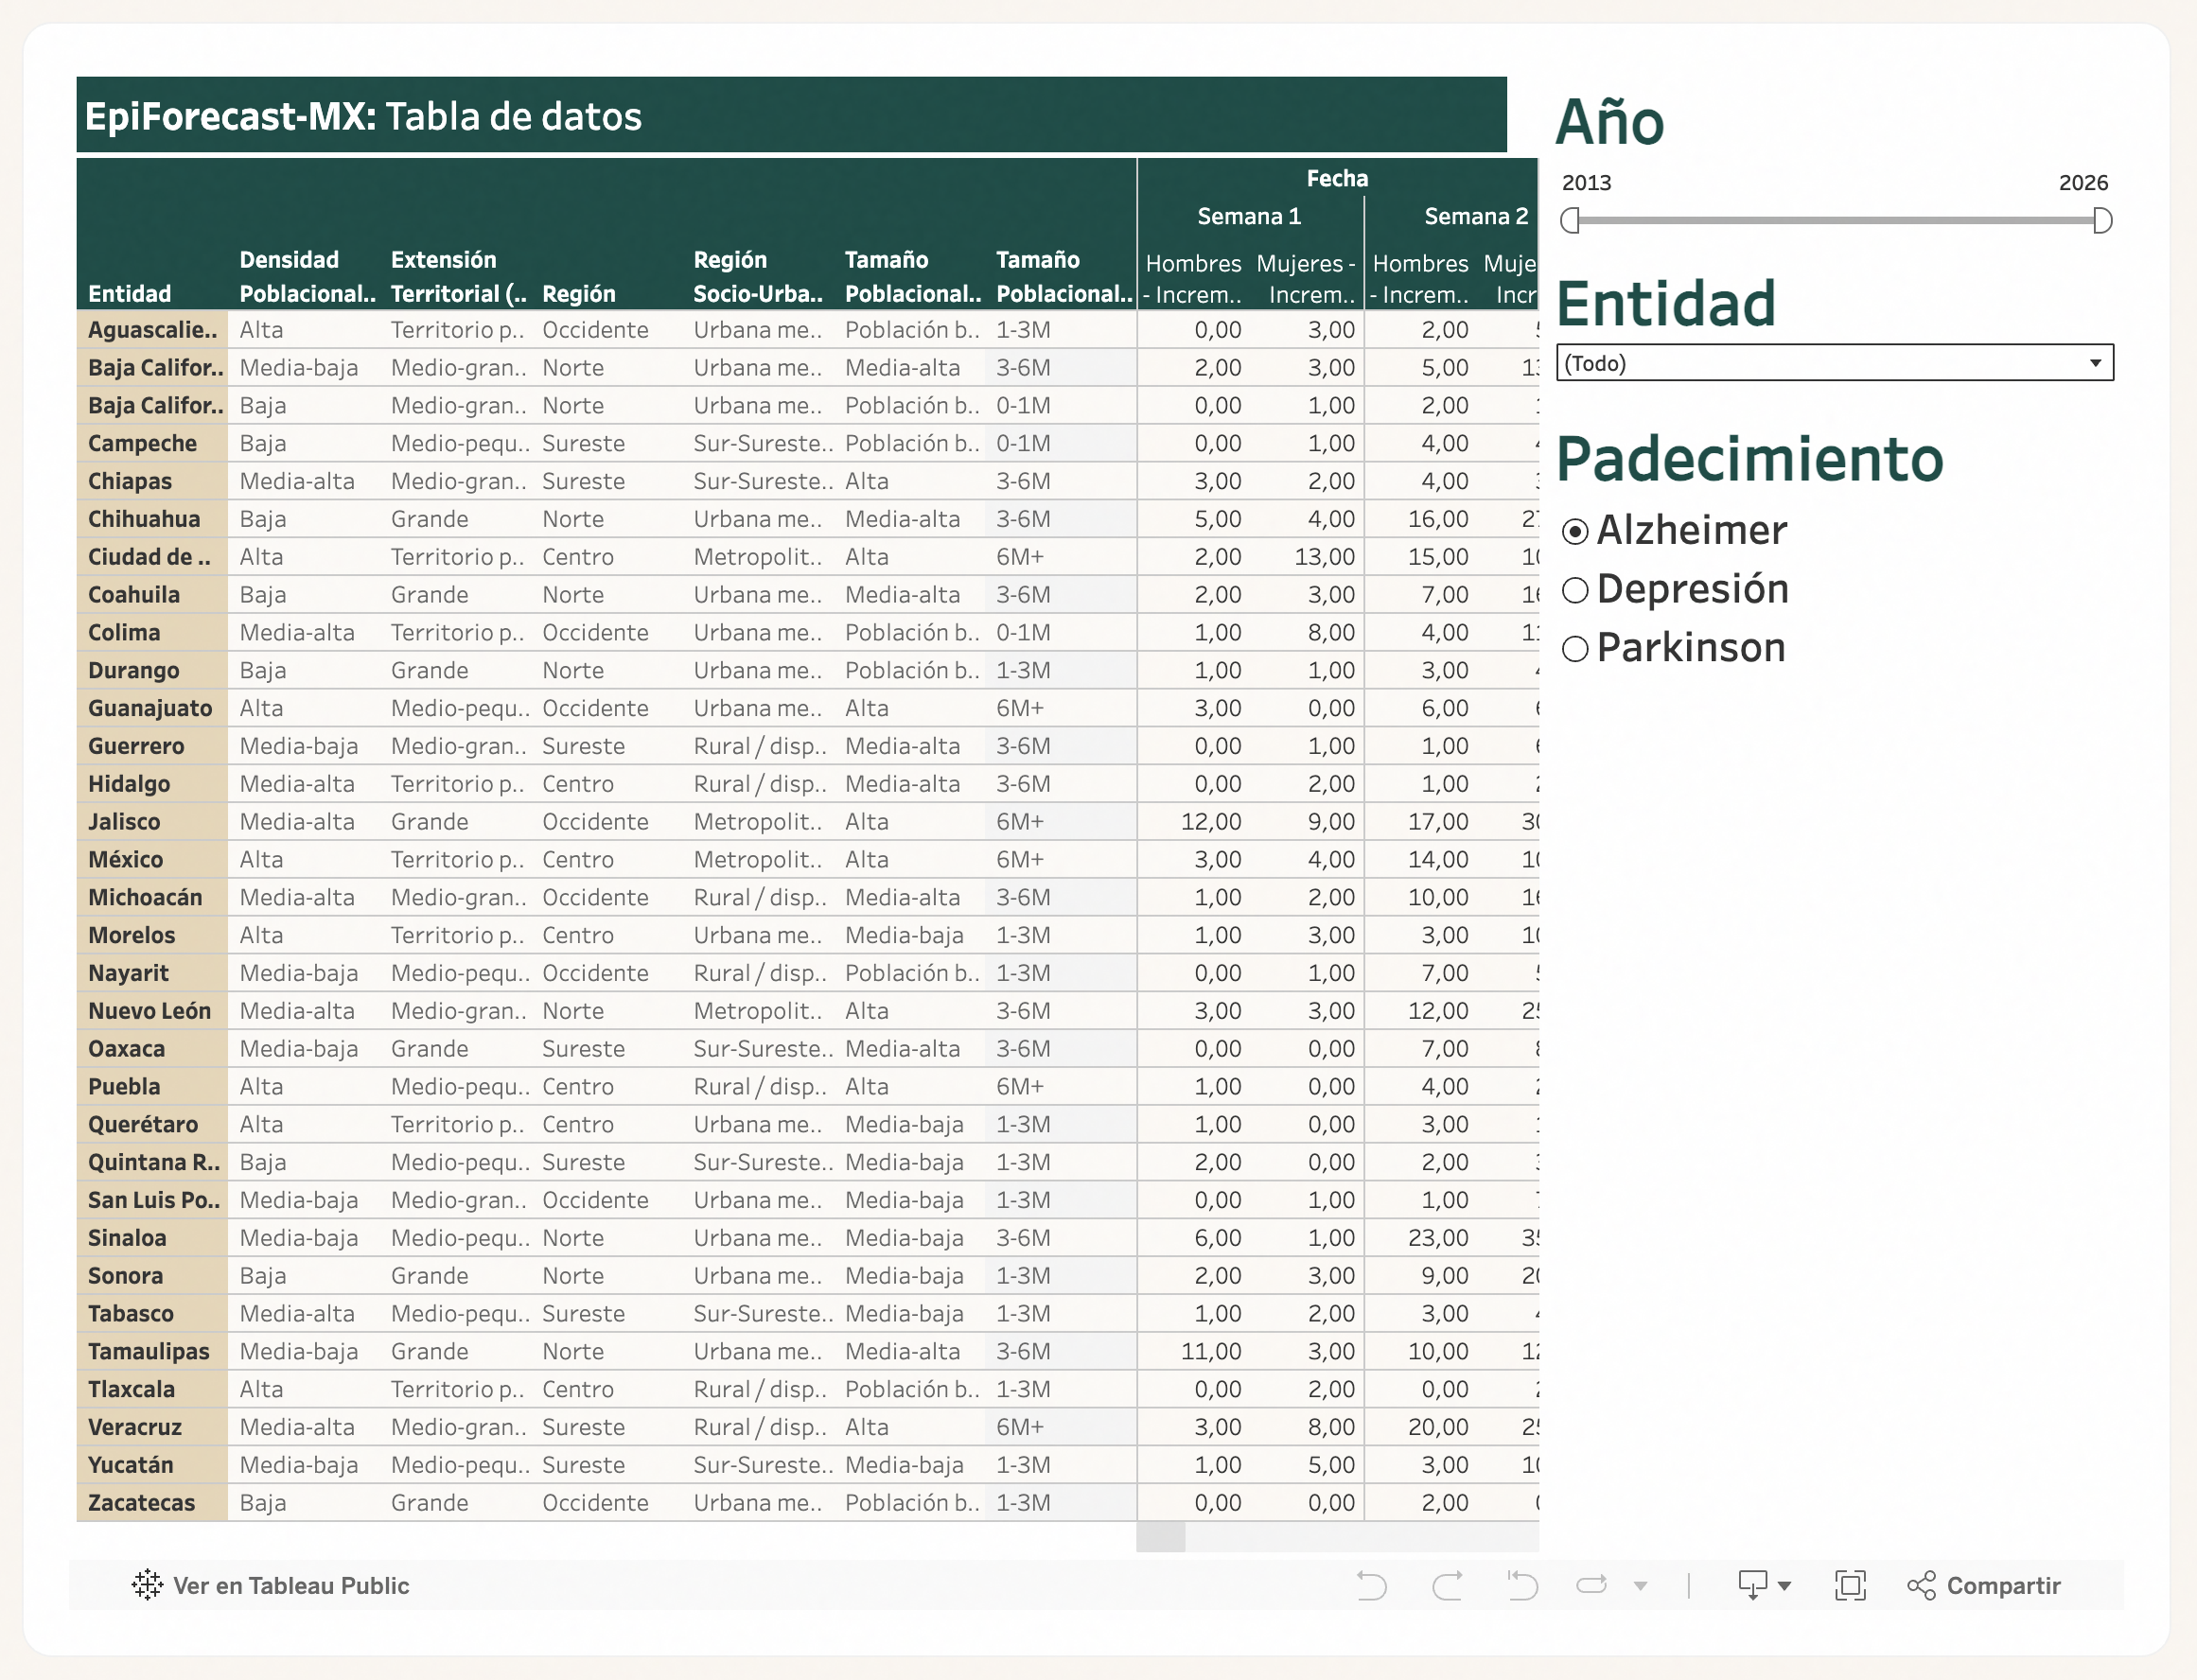
\includegraphics[width=0.75\textwidth]{tabla2.png}
\caption{Dashboard Tableau — Filtros de padecimiento (selección única) y entidad federativa con estandarización tipográfica.}
\label{fig:tableau-filtros}
\end{figure}

\subsection{Normalización Cromática Min-Max}\label{sec:tableau-norm}

Para la visualización de mapas que alternan entre variables continuas (densidad poblacional, incrementos de casos, superficie territorial), se implementó una normalización min-max exclusivamente para fines de representación cromática:

\begin{equation}
x_{\text{norm}} = \frac{x - \min(x)}{\max(x) - \min(x)}
\label{eq:minmax}
\end{equation}

En Tableau, la implementación robusta con agregación y protección contra división entre cero se expresa como:

\begin{lstlisting}[caption={Normalización min-max en Tableau (ejemplo con Densidad Territorial).}]
IF
    { FIXED : MAX(SUM([Densidad Territorial])) }
    = { FIXED : MIN(SUM([Densidad Territorial])) }
THEN
    0
ELSE
    ( SUM([Densidad Territorial])
      - { FIXED : MIN(SUM([Densidad Territorial])) } )
    /
    ( { FIXED : MAX(SUM([Densidad Territorial])) }
      - { FIXED : MIN(SUM([Densidad Territorial])) } )
END
\end{lstlisting}

Esta transformación permite que el gradiente de color sea consistente al alternar variables, garantizando una lectura visual homogénea. El valor real no normalizado se incorpora en el tooltip para preservar la interpretación cuantitativa.

\begin{figure}[H]
\centering
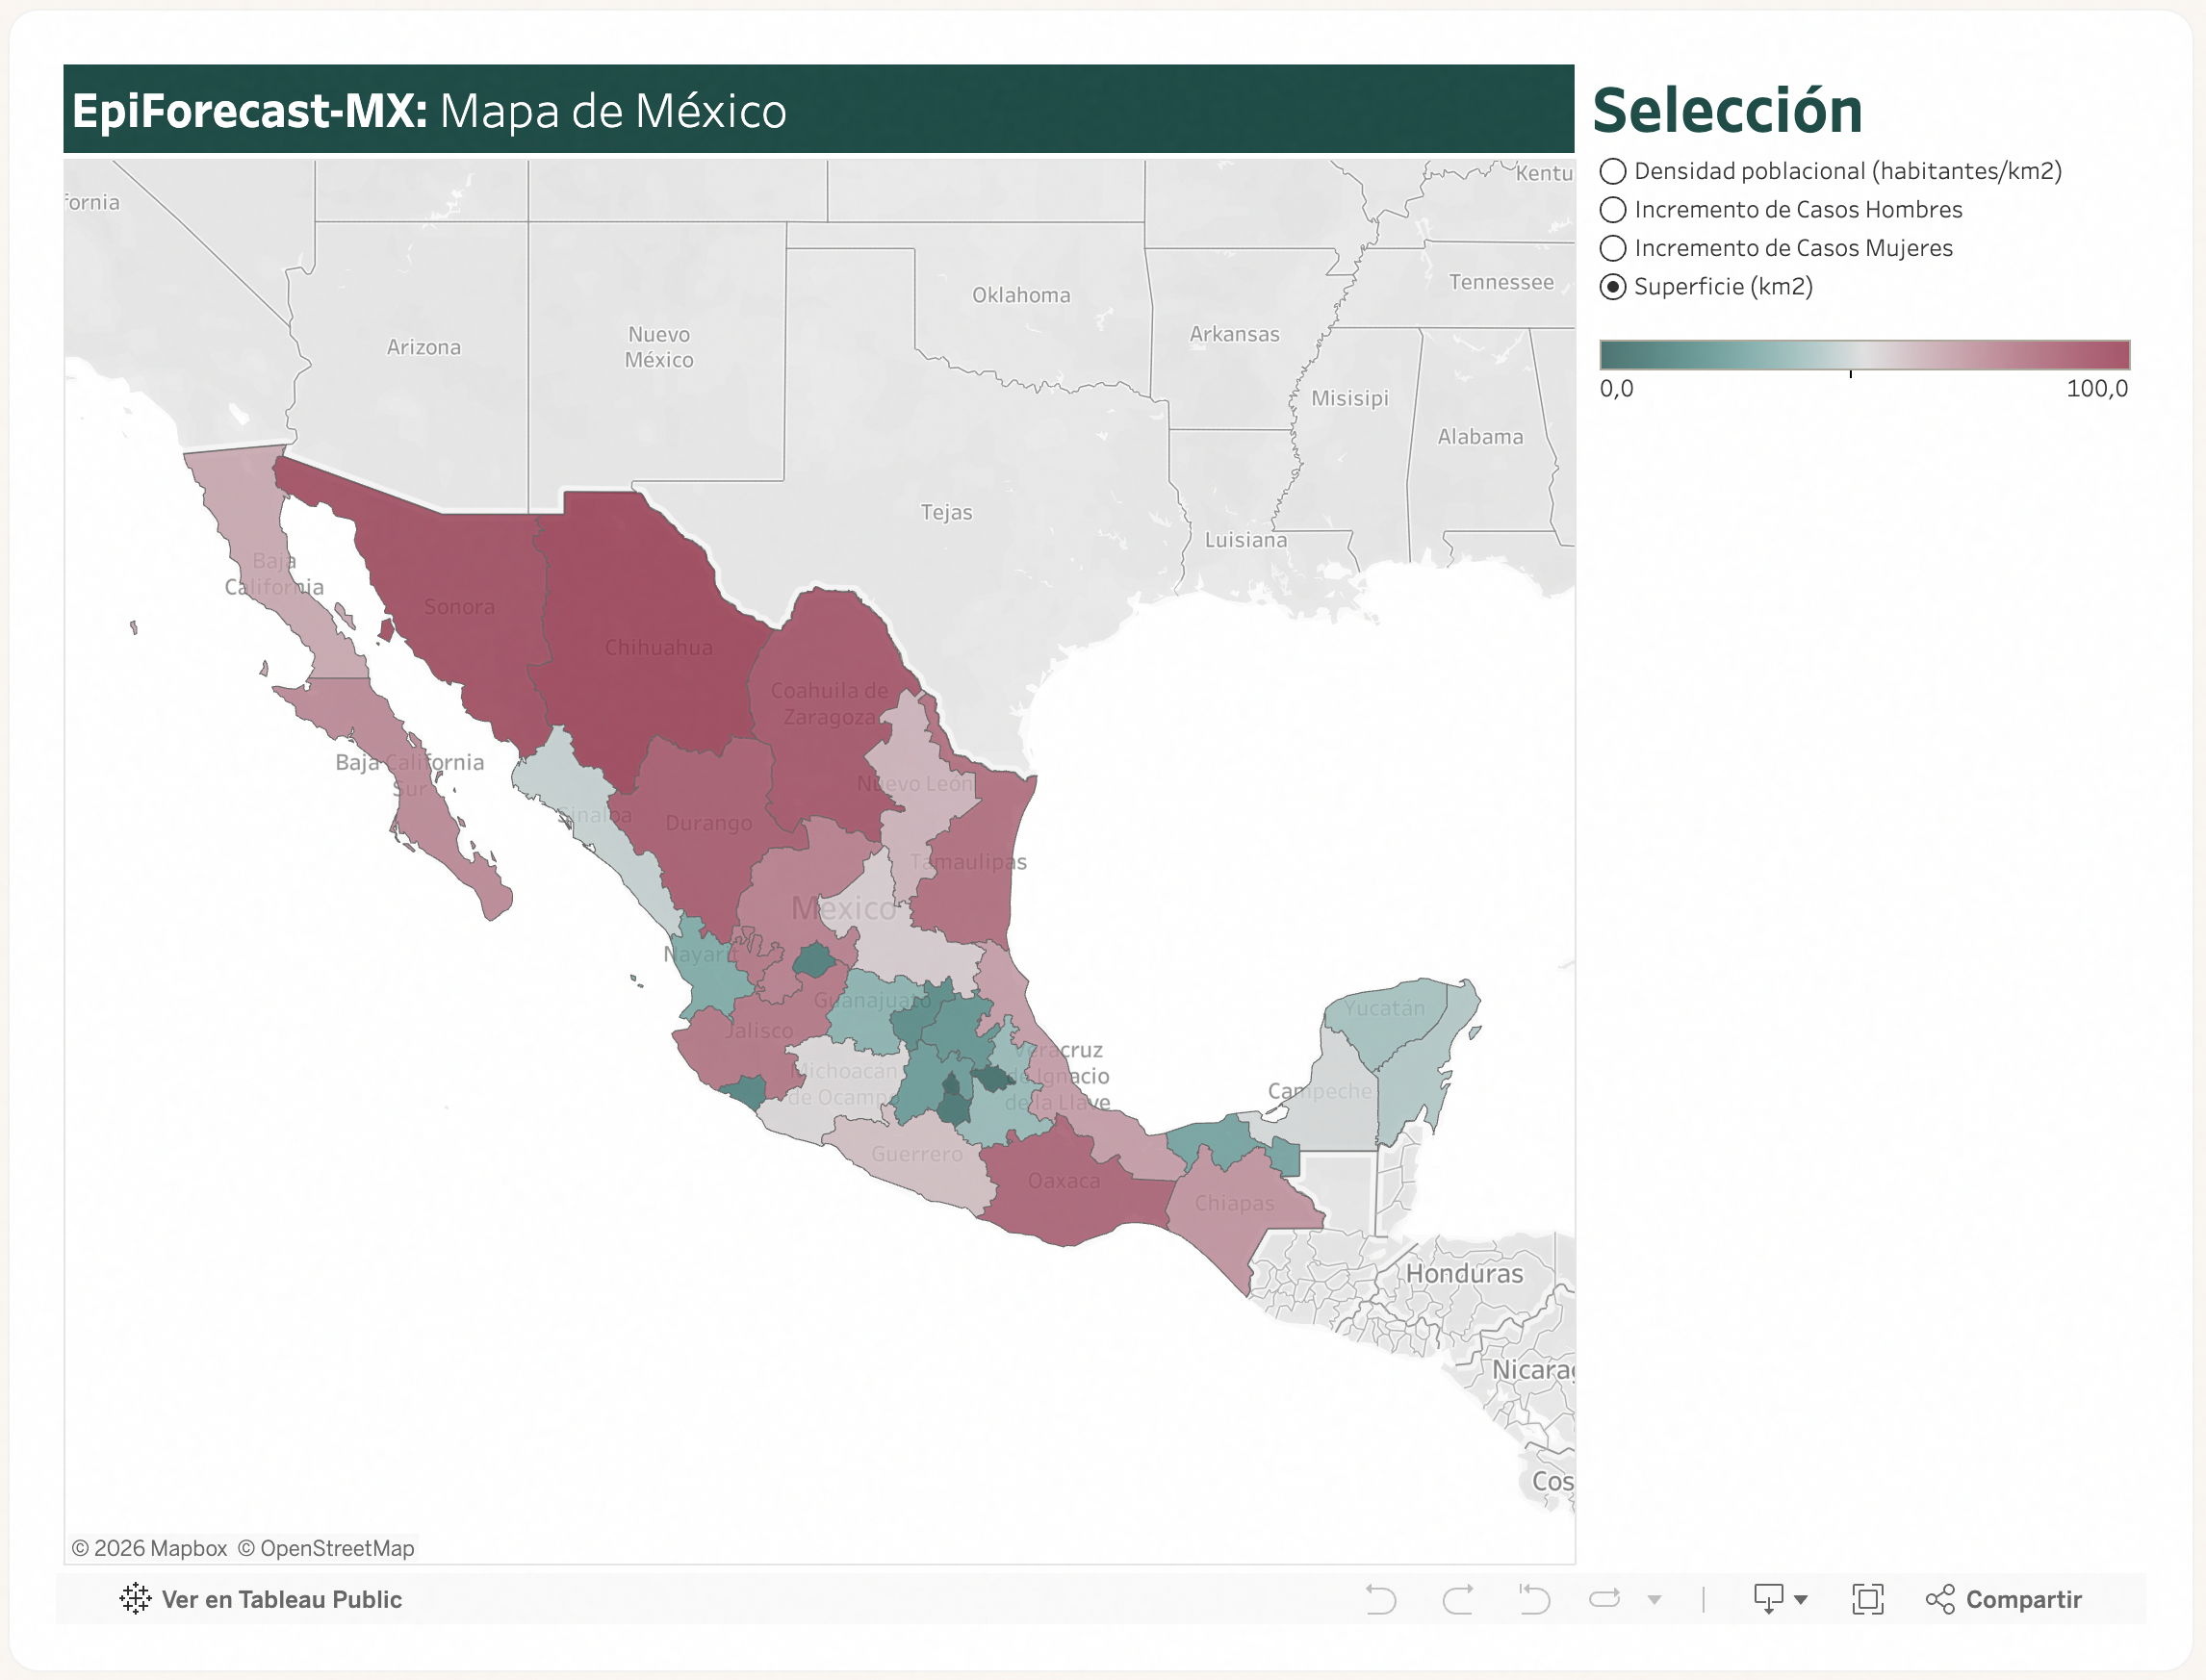
\includegraphics[width=0.75\textwidth]{mapa2.png}
\caption{Mapa coroplético con normalización min-max. El gradiente de color refleja la posición relativa dentro de la distribución de la variable seleccionada; el tooltip muestra el valor real sin normalizar.}
\label{fig:tableau-mapa}
\end{figure}

\subsection{Tasas Normalizadas y Recorte Visual de Valores Extremos}\label{sec:tableau-tasas}

El indicador principal se define como una tasa de incremento de casos por cada 100,000~habitantes, calculada a nivel agregado:

\begin{equation}
\text{Tasa}_{100k} = \frac{\sum \text{Casos}}{\sum \text{Población}} \times 100{,}000
\label{eq:tasa}
\end{equation}

Para mitigar la distorsión visual producida por valores extremos (particularmente en la captura anormal de 2016), se implementó un recorte visual (\emph{capping}) basado en el percentil~99:

\begin{equation}
\text{Valor}_{\text{cap}} =
\begin{cases}
\text{Tasa}_{100k}, & \text{si } \text{Tasa}_{100k} \le P_{99} \\
P_{99}, & \text{si } \text{Tasa}_{100k} > P_{99}
\end{cases}
\label{eq:capping}
\end{equation}

La implementación en Tableau utiliza \texttt{WINDOW\_PERCENTILE()} como \emph{table calculation} dinámica:

\begin{lstlisting}[caption={Recorte visual con percentil~99 en Tableau (ejemplo para hombres).}]
IF
    ( (SUM([Hombres - Incrementos de casos])
       / SUM([Habitantes (Hombres)])) * 100000 )
    <= WINDOW_PERCENTILE(
        ( (SUM([Hombres - Incrementos de casos])
           / SUM([Habitantes (Hombres)])) * 100000 ),
        0.99
    )
THEN
    (SUM([Hombres - Incrementos de casos])
     / SUM([Habitantes (Hombres)])) * 100000
ELSE
    WINDOW_PERCENTILE(
        ( (SUM([Hombres - Incrementos de casos])
           / SUM([Habitantes (Hombres)])) * 100000 ),
        0.99
    )
END
\end{lstlisting}

La configuración de \texttt{Compute Using} se ajusta según la escala temporal: dimensión anual para series anuales y dimensión semanal para series semanales, garantizando que el percentil~99 se calcule sobre el conjunto temporal correcto.

\begin{figure}[H]
\centering
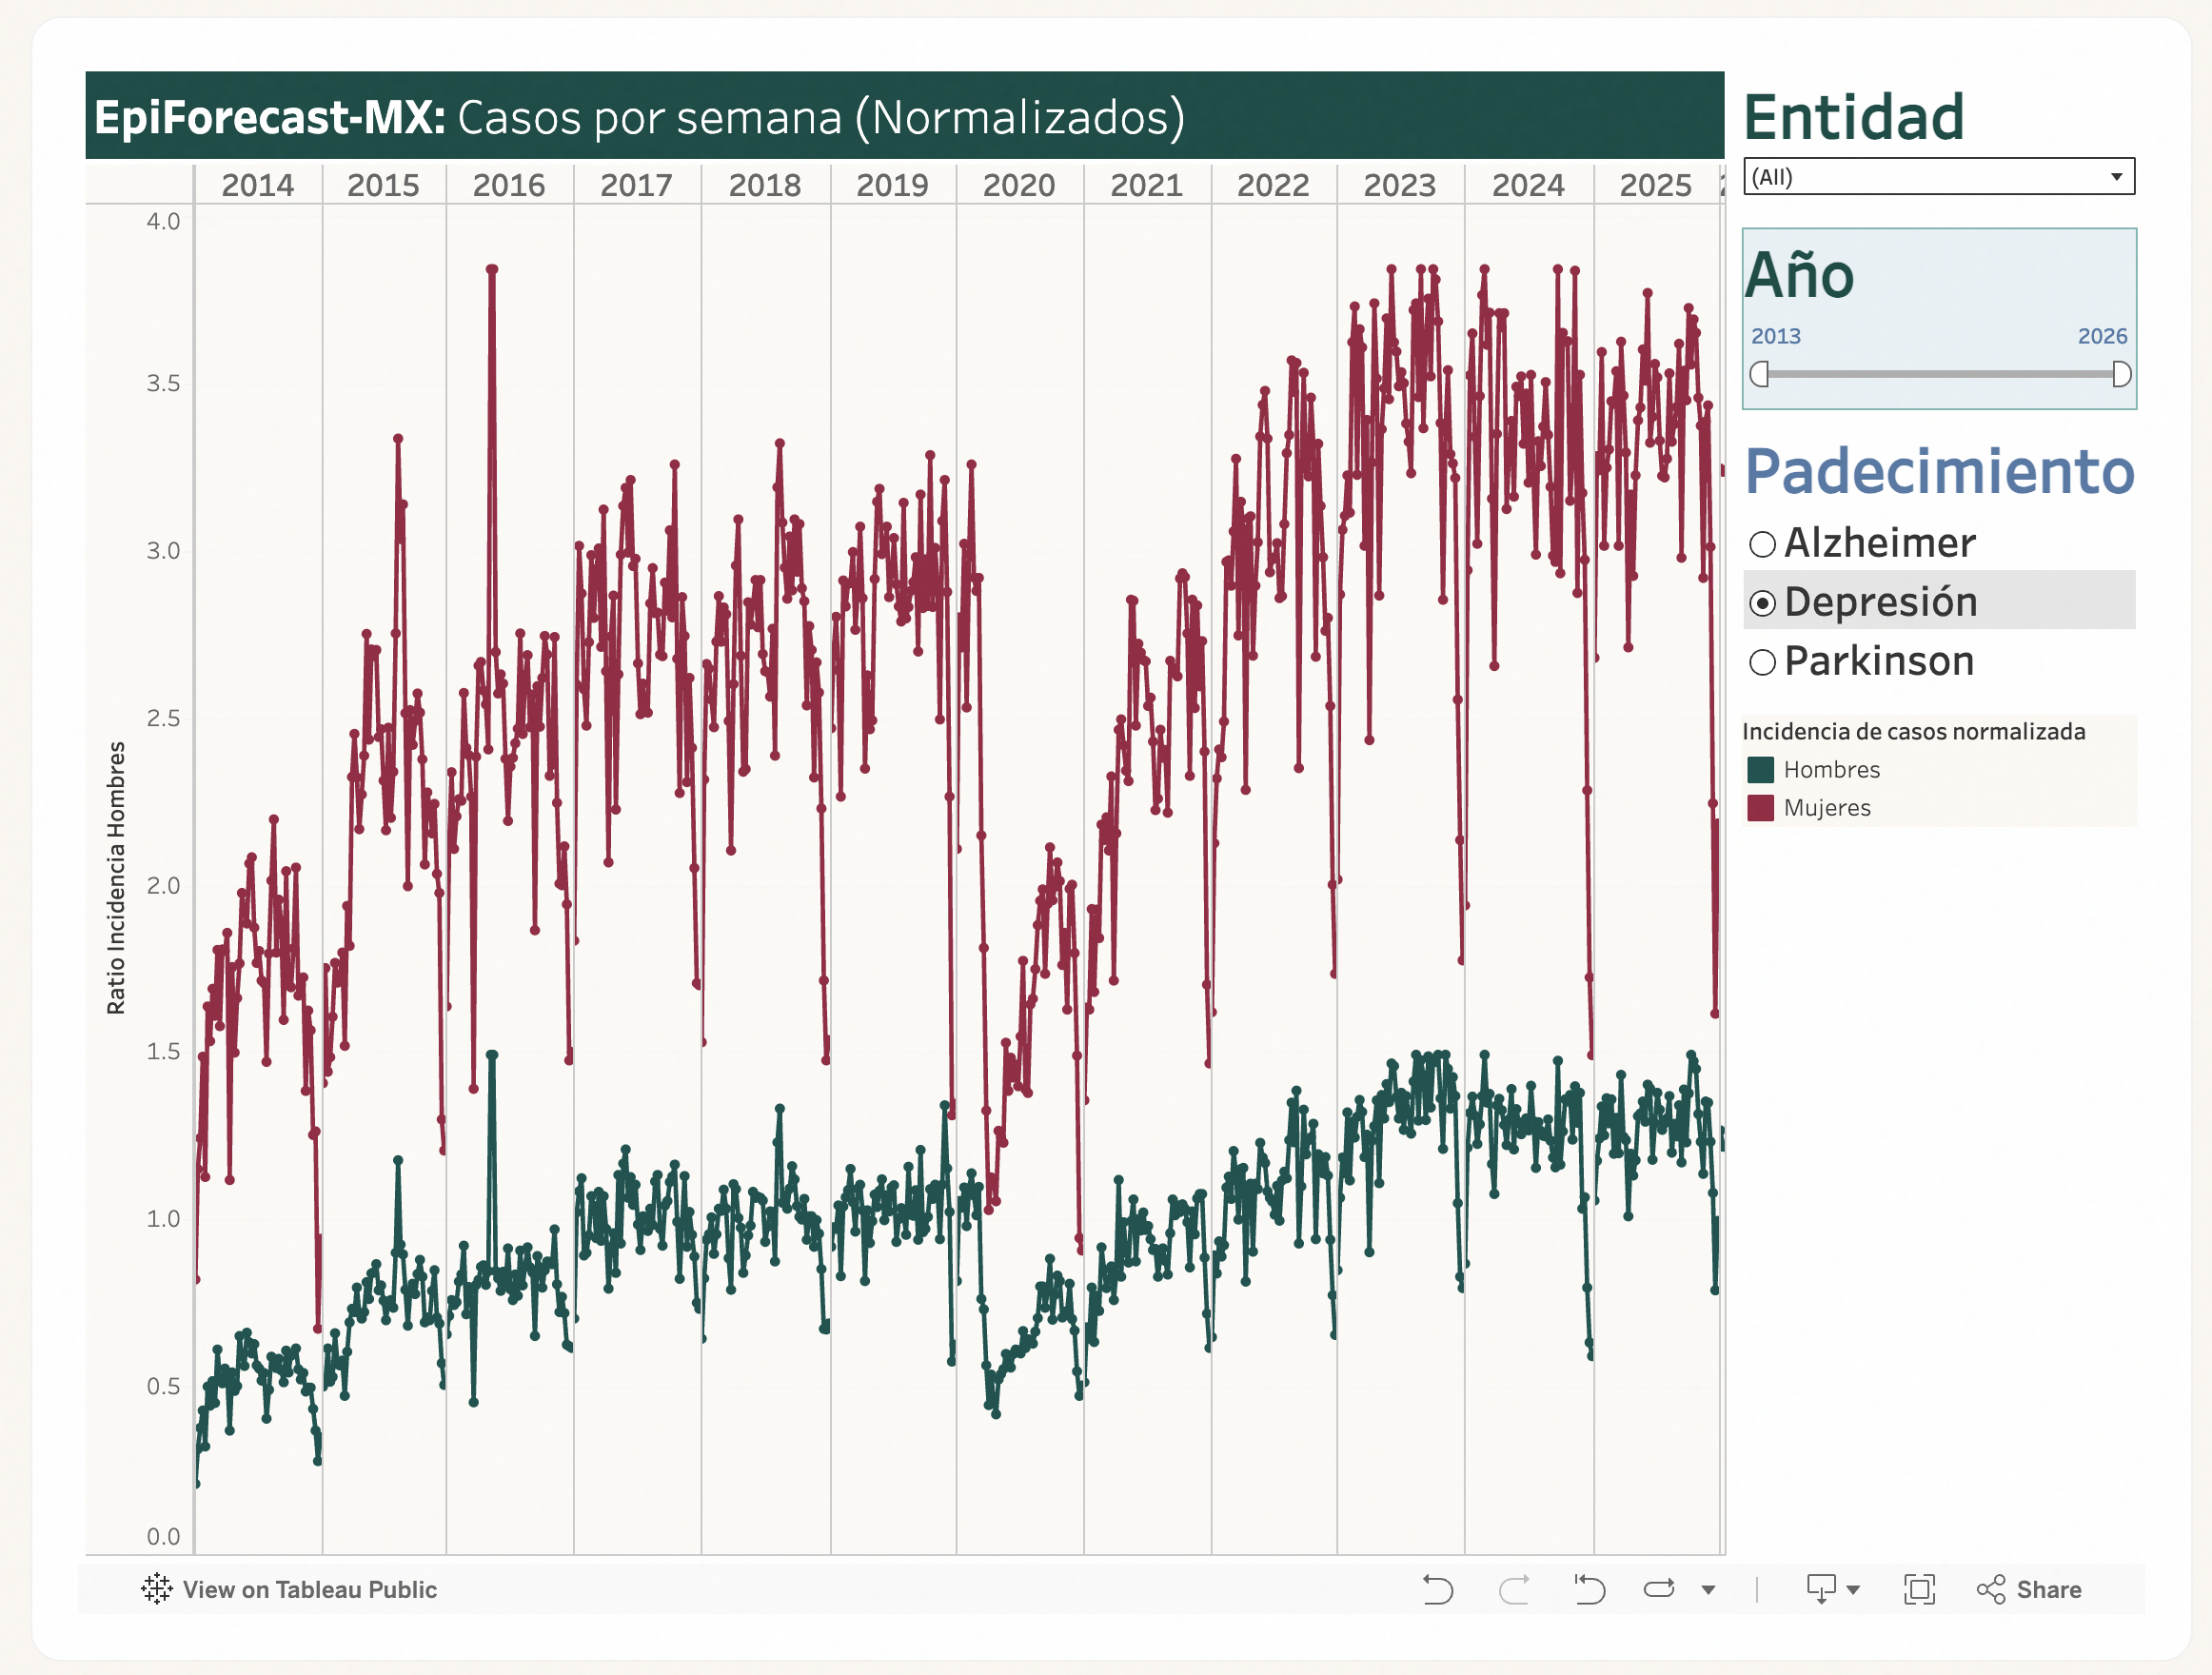
\includegraphics[width=0.75\textwidth]{norm1.png}
\caption{Serie temporal antes del recorte visual — los valores extremos de 2016 comprimen la escala vertical y ocultan las tendencias relevantes.}
\label{fig:tableau-norm1}
\end{figure}

\begin{figure}[H]
\centering
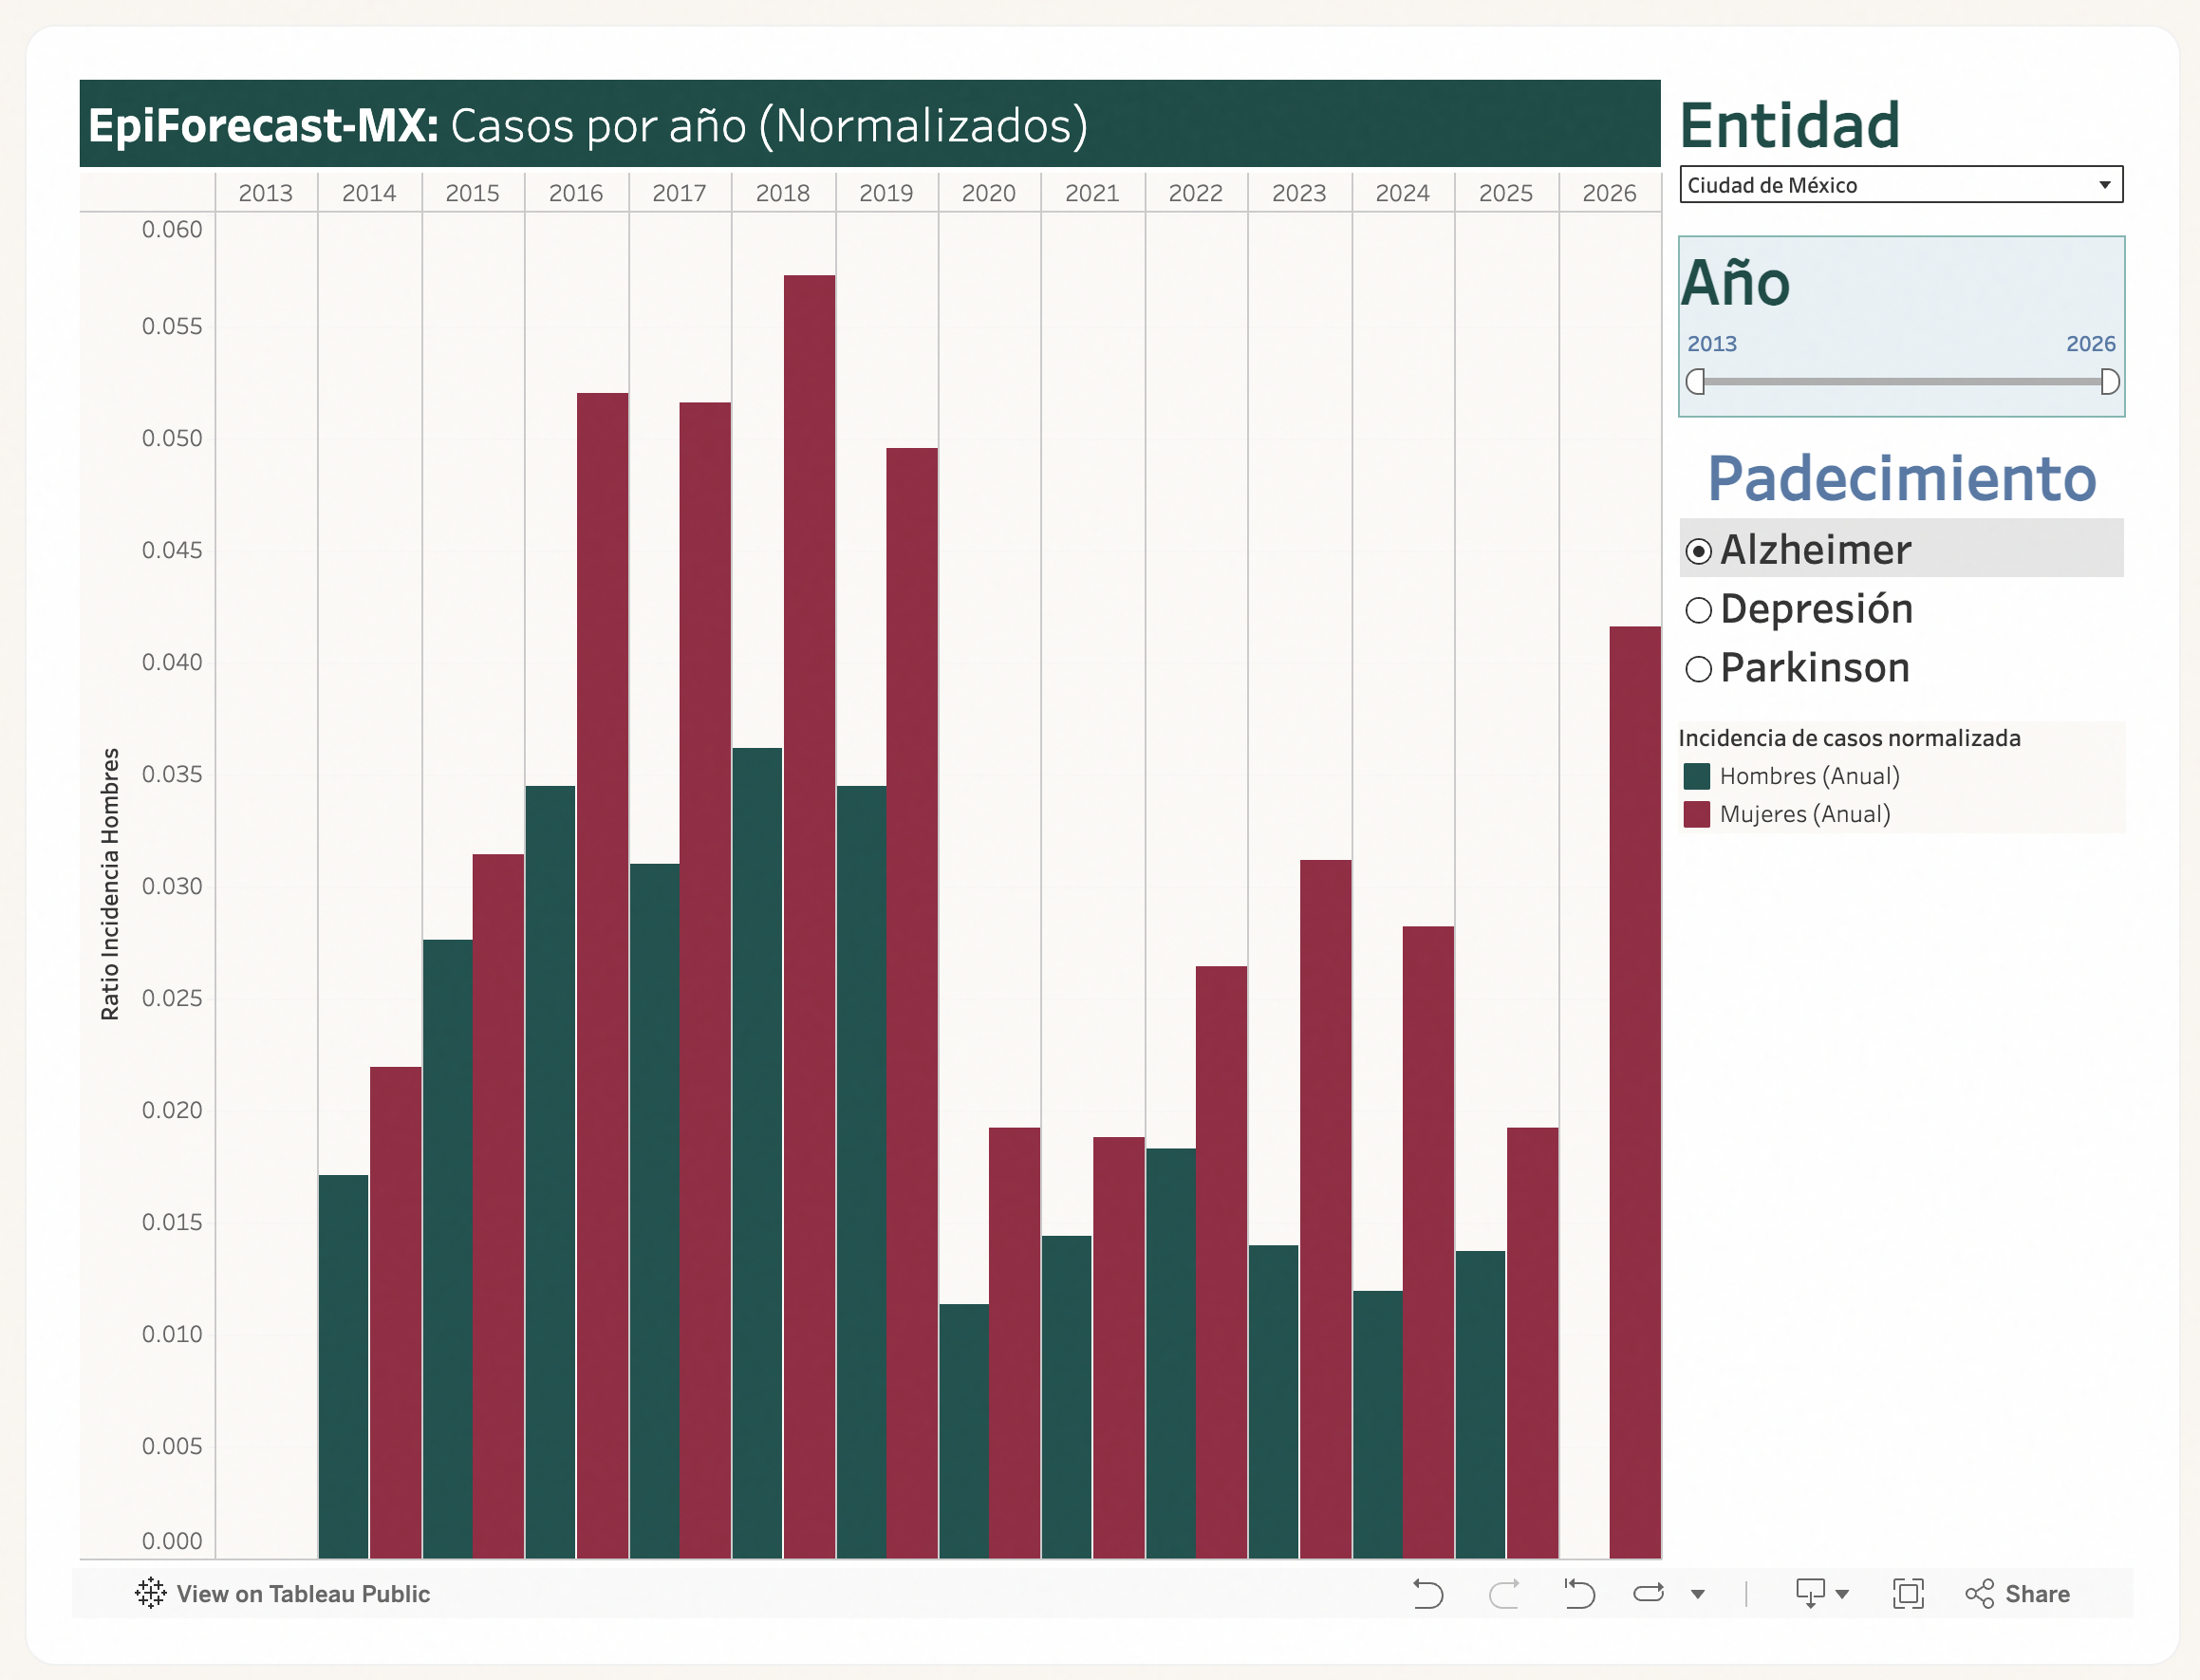
\includegraphics[width=0.75\textwidth]{norm2.png}
\caption{Serie temporal con \emph{capping} al percentil~99 aplicado. La escala vertical permite observar las variaciones estacionales y la disrupción COVID-19 sin distorsión por outliers extremos.}
\label{fig:tableau-norm2}
\end{figure}

% =============================================================================
%  10. CONCLUSIONES Y SIGUIENTES PASOS
% =============================================================================
\section{Conclusiones y Siguientes Pasos}\label{sec:conclusiones}

\subsection{Hallazgos Principales}

El desarrollo y evaluación de 297 modelos baseline permite establecer las siguientes conclusiones:

\textbf{Viabilidad confirmada para los tres padecimientos.} Prophet captura la dinámica temporal de Depresión, Parkinson y Alzheimer. El desempeño del baseline supera consistentemente al modelo naïve, validando la capacidad predictiva del enfoque propuesto.

\textbf{Cada padecimiento tiene un comportamiento epidemiológico distinto.} Se justifica plenamente la separación en modelos independientes, tal como recomendó la Dra.\ Grettel. Depresión muestra la mayor dominancia de tendencia (82.4\%), Parkinson un balance intermedio (60.3\%/39.7\%), y Alzheimer una preponderancia de la estacionalidad (54.4\%).

\textbf{El efecto COVID-19 fue capturado.} Los \emph{changepoints} detectados coinciden con el período de emergencia sanitaria (marzo 2020 -- junio 2021), validando la robustez del algoritmo ante quiebres estructurales.

\textbf{Variabilidad significativa entre estados.} La dispersión del MAPE estatal (desde 4.79\% en Ciudad de México hasta 102.27\% en Puebla) valida la decisión de entrenar modelos individuales por entidad y señala las diferencias en infraestructura de captura de datos.

\textbf{Diferencias por sexo documentadas.} Los modelos desagregados evidencian niveles de predecibilidad distintos entre hombres y mujeres, información relevante para la asignación diferenciada de recursos solicitada por las stakeholders del IMSS.

\textbf{Outliers identificados y contextualizados.} La detección sistemática mediante IQR identificó 143~outliers en Depresión, 36 en Parkinson y 0 en Alzheimer, permitiendo distinguir entre variabilidad epidemiológica genuina y anomalías en el reporte.

\subsection{Del Baseline al Modelo Tuneado (Avance~4)}

La Tabla~\ref{tab:tuning} presenta el espacio de exploración de hiperparámetros previsto para el Avance~4.

\begin{table}[H]
\centering
\caption{Hiperparámetros baseline y espacio de exploración para el Avance~4.}
\label{tab:tuning}
\small
\begin{tabularx}{\textwidth}{@{}l l X@{}}
\toprule
\textbf{Hiperparámetro} & \textbf{Valor Baseline} & \textbf{Exploración Avance~4} \\
\midrule
\texttt{seasonality\_mode} & \texttt{additive} & \texttt{multiplicative} para estados con estacionalidad proporcional \\
\texttt{changepoint\_prior\_scale} & 0.05 & Grid: [0.01, 0.05, 0.1, 0.5, 1.0] \\
\texttt{seasonality\_prior\_scale} & 10.0 & Grid: [0.1, 0.5, 1.0, 5.0, 10.0] \\
\texttt{holidays} & ninguno & Días festivos mexicanos y períodos vacacionales \\
\texttt{regressors} & ninguno & Variables exógenas (densidad, región socioeconómica) \\
\bottomrule
\end{tabularx}
\end{table}

\subsection{Alineación con Objetivos Estratégicos}

Desde la perspectiva académica, este avance cumple los objetivos~3.1 y 3.2 del Módulo~3 (TC5035): métricas de calidad establecidas y modelo de referencia funcional. Desde la perspectiva científica, constituye una línea base reproducible para los dos artículos en desarrollo y los congresos internacionales de Estocolmo y Portugal. Desde la perspectiva operativa, los pronósticos baseline son potencialmente útiles para planificación inicial en el IMSS; los modelos tuneados del Avance~4 mejorarán la precisión para uso institucional.

% =============================================================================
%  11. REFLEXIONES INDIVIDUALES
% =============================================================================
\section{Reflexiones Individuales}\label{sec:reflexiones}

\begin{wrapfigure}{l}{3.5cm}
    \vspace{-0.4cm}
    \centering
    
\includegraphics[width=3.2cm, height=3.2cm, keepaspectratio]{JARS3.png}
    \vspace{-0.4cm}
\end{wrapfigure}
\textbf{Javier Augusto Rebull Saucedo} --- \textit{``El Avance~3 representó un punto de inflexión en mi comprensión del proyecto. Diseñar y ejecutar 297~modelos baseline me obligó a pensar en escalabilidad desde el código: funciones reutilizables, pipelines parametrizados y visualizaciones que se generan automáticamente para cualquier combinación de padecimiento, estado y sexo. La retroalimentación de la Dra.\ Grettel sobre la necesidad de separar los padecimientos fue determinante; al modelarlos independientemente, las diferencias epidemiológicas entre Depresión, Parkinson y Alzheimer se hicieron evidentes no solo en las métricas, sino en la estructura misma de las series. Uno de los aprendizajes más valiosos fue entender que un baseline no es un modelo `malo' que se descarta: es la referencia objetiva que da sentido a toda optimización posterior. Además, la implementación del dashboard ejecutivo y las cuadrículas comparativas me enseñó que la comunicación visual de resultados es tan importante como los resultados mismos, especialmente cuando los stakeholders son médicos, no ingenieros.''}
\vspace{1em}

\begin{wrapfigure}{l}{3.5cm}
    \vspace{-0.4cm}
    \centering
    \includegraphics[width=3.2cm, height=3.2cm, keepaspectratio]{JARCOS3.png}
    \vspace{-0.4cm}
\end{wrapfigure}
\textbf{Juan Carlos Pérez Nava} --- \textit{``Como profesional de TI en el IMSS, este avance tiene un significado particular: estamos construyendo herramientas que podrían integrarse directamente en los procesos de planificación institucional. La validación cruzada temporal me permitió entender la importancia de evaluar modelos de manera realista —no con splits aleatorios que violan la temporalidad de los datos, sino con ventanas deslizantes que simulan el escenario real de pronóstico—. La detección de outliers fue reveladora: muchos de los valores atípicos coinciden con períodos de captura irregular que conozco de primera mano por mi trabajo en la institución. Esto refuerza la necesidad de que el sistema de pronóstico sea robusto ante las imperfecciones reales de los datos epidemiológicos. El hecho de que Prophet capture los changepoints del COVID-19 sin intervención manual valida su idoneidad para un entorno donde los quiebres estructurales no se pueden anticipar. De cara al Avance~4, mi principal interés es explorar cómo la incorporación de variables exógenas —particularmente las que manejamos internamente en el IMSS— puede mejorar la precisión estatal.''}
\vspace{1em}

\begin{wrapfigure}{l}{3.5cm}
    \vspace{-0.4cm}
    \centering
    
\includegraphics[width=3.2cm, height=3.2cm, keepaspectratio]{Luis3.png}
    \vspace{-0.4cm}
\end{wrapfigure}
\textbf{Luis Gerardo Sánchez Salazar} --- \textit{``Mi experiencia en ingeniería de controles en Tesla me ha dado una perspectiva particular sobre sistemas dinámicos, y las series de tiempo epidemiológicas comparten más de lo esperado con los sistemas que modelo profesionalmente: tendencias, estacionalidades, perturbaciones externas y la necesidad de intervalos de confianza para la toma de decisiones. El aspecto que más me impactó de este avance fue la heterogeneidad entre estados. Mientras que algunos estados presentan series limpias y predecibles (MAPE~$<$~20\%), otros son prácticamente impredecibles con un modelo baseline, lo cual apunta directamente a diferencias en la infraestructura de captura de datos, no necesariamente en la dinámica epidemiológica subyacente. La construcción del dashboard y las visualizaciones comparativas del Tableau me reforzaron la importancia de traducir resultados técnicos a formatos consumibles por tomadores de decisiones. El Avance~4 será la prueba de fuego: ¿cuánto podemos mejorar con tuning inteligente de hiperparámetros y qué estados realmente se beneficiarán del ajuste fino?''}

% =============================================================================
%  REFERENCIAS
% =============================================================================
\newpage
\section{Referencias}\label{sec:referencias}

\begingroup
\renewcommand{\section}[2]{}% Suprimir título de bibliografía
\begin{thebibliography}{99}

% --- Algoritmo y Metodología ---
\bibitem[Taylor y Letham(2018)]{taylor2018forecasting}
Taylor, S.~J. y Letham, B. (2018).
\newblock Forecasting at scale.
\newblock \emph{The American Statistician}, \emph{72}(1), 37--45.
\newblock \url{https://doi.org/10.1080/00031305.2017.1380080}

\bibitem[Studer et~al.(2021)]{studer2021crisp}
Studer, S., Bui, T.~B., Drescher, C., Hanuschkin, A., Winkler, L., Peters, S. y Müller, K.-R. (2021).
\newblock Towards CRISP-ML(Q): A machine learning process model with quality assurance methodology.
\newblock \emph{Machine Learning and Knowledge Extraction}, \emph{3}(2), 392--413.
\newblock \url{https://doi.org/10.3390/make3020020}

\bibitem[Géron(2022)]{geron2022hands}
Géron, A. (2022).
\newblock \emph{Hands-on machine learning with Scikit-Learn, Keras, and TensorFlow} (3.ª~ed.).
\newblock O'Reilly Media.

% --- Métricas de Desempeño y Validación ---
\bibitem[Hyndman y Koehler(2006)]{hyndman2006another}
Hyndman, R.~J. y Koehler, A.~B. (2006).
\newblock Another look at measures of forecast accuracy.
\newblock \emph{International Journal of Forecasting}, \emph{22}(4), 679--688.
\newblock \url{https://doi.org/10.1016/j.ijforecast.2006.03.001}

\bibitem[Hyndman y Athanasopoulos(2021)]{hyndman2021forecasting}
Hyndman, R.~J. y Athanasopoulos, G. (2021).
\newblock \emph{Forecasting: Principles and practice} (3.ª~ed.).
\newblock OTexts.
\newblock \url{https://otexts.com/fpp3/}

\bibitem[Bergmeir y Benítez(2012)]{bergmeir2012use}
Bergmeir, C. y Benítez, J.~M. (2012).
\newblock On the use of cross-validation for time series predictor evaluation.
\newblock \emph{Information Sciences}, \emph{191}, 192--213.
\newblock \url{https://doi.org/10.1016/j.ins.2011.12.028}

% --- Sub/Sobreajuste y Selección de Modelos ---
\bibitem[Hastie et~al.(2009)]{hastie2009elements}
Hastie, T., Tibshirani, R. y Friedman, J. (2009).
\newblock \emph{The elements of statistical learning: Data mining, inference, and prediction} (2.ª~ed.).
\newblock Springer.
\newblock \url{https://doi.org/10.1007/978-0-387-84858-7}

\bibitem[James et~al.(2021)]{james2021introduction}
James, G., Witten, D., Hastie, T. y Tibshirani, R. (2021).
\newblock \emph{An introduction to statistical learning with applications in R} (2.ª~ed.).
\newblock Springer.
\newblock \url{https://doi.org/10.1007/978-1-0716-1418-1}

% --- Detección de Outliers y Descomposición ---
\bibitem[Tukey(1977)]{tukey1977exploratory}
Tukey, J.~W. (1977).
\newblock \emph{Exploratory data analysis}.
\newblock Addison-Wesley.

\bibitem[Cleveland et~al.(1990)]{cleveland1990stl}
Cleveland, R.~B., Cleveland, W.~S., McRae, J.~E. y Terpenning, I. (1990).
\newblock STL: A seasonal-trend decomposition procedure based on loess.
\newblock \emph{Journal of Official Statistics}, \emph{6}(1), 3--33.

% --- Epidemiología en México ---
\bibitem[Morales-Chainé et~al.(2023)]{morales2023incidence}
Morales-Chainé, S., López-Montoya, A., Bosch-Maldonado, A., Beristain-Aguirre, A., Robles-García, R. y López-Rosales, F. (2023).
\newblock Incidence of depression and suicide rate in Mexico.
\newblock \emph{Salud Mental}, \emph{46}(5), 131--139.
\newblock \url{https://doi.org/10.17711/SM.0185-3325.2023.017}

\bibitem[Romero-Guerrero et~al.(2024)]{romero2024prevalencia}
Romero-Guerrero, X.~R., Cortés-García, H., Alcántar-Chávez, F., Miranda-García, M., Almazán-Farfán, V. y Victoria-Carrasco, O.~Y. (2024).
\newblock Prevalencia relacionada a trastornos mentales y del comportamiento en población derechohabiente del IMSS, 2021.
\newblock \emph{Revista Médica del Instituto Mexicano del Seguro Social}, \emph{62}(3), 1--8.
\newblock \url{https://doi.org/10.5281/zenodo.10998791}

% --- Impacto del COVID-19 ---
\bibitem[Antonio-Villa et~al.(2022)]{antoniovilla2022socio}
Antonio-Villa, N.~E., Bello-Chavolla, O.~Y., Fermín-Martínez, C.~A., Aburto, J.~M., Fernández-Chirino, L., Ramírez-García, D., \ldots\ y Barquera, S. (2022).
\newblock Socio-demographic inequalities and excess non-COVID-19 mortality during the COVID-19 pandemic: A data-driven analysis of 1,069,174 death certificates in Mexico.
\newblock \emph{International Journal of Epidemiology}, \emph{51}(6), 1711--1723.
\newblock \url{https://doi.org/10.1093/ije/dyac184}

\bibitem[Hernández-Díaz et~al.(2022)]{hernandez2022mental}
Hernández-Díaz, Y., Genis-Mendoza, A.~D., Ramos-Méndez, M.~A., Juárez-Rojop, I.~E., Tovilla-Zárate, C.~A., González-Castro, T.~B., López-Narváez, M.~L. y Nicolini, H. (2022).
\newblock Mental health impact of the COVID-19 pandemic on Mexican population: A systematic review.
\newblock \emph{International Journal of Environmental Research and Public Health}, \emph{19}(11), 6953.
\newblock \url{https://doi.org/10.3390/ijerph19116953}

% --- Normalización Epidemiológica y Visualización ---
\bibitem[Rothman et~al.(2008)]{rothman2008modern}
Rothman, K.~J., Greenland, S. y Lash, T.~L. (2008).
\newblock \emph{Modern epidemiology} (3.ª~ed.).
\newblock Lippincott Williams \& Wilkins.

\bibitem[Few(2006)]{few2006information}
Few, S. (2006).
\newblock \emph{Information dashboard design: The effective visual communication of data}.
\newblock O'Reilly Media.

\bibitem[Midway(2020)]{midway2020principles}
Midway, S.~R. (2020).
\newblock Principles of effective data visualization.
\newblock \emph{Patterns}, \emph{1}(9), 100141.
\newblock \url{https://doi.org/10.1016/j.patter.2020.100141}

% --- MLOps y Reproducibilidad ---
\bibitem[Kreuzberger et~al.(2023)]{kreuzberger2023mlops}
Kreuzberger, D., Kühl, N. y Hirschl, S. (2023).
\newblock Machine learning operations (MLOps): Overview, definition, and architecture.
\newblock \emph{IEEE Access}, \emph{11}, 31866--31879.
\newblock \url{https://doi.org/10.1109/ACCESS.2023.3262138}

\bibitem[Visengeriyeva(2023)]{visengeriyeva2023crisp}
Visengeriyeva, L. (2023).
\newblock \emph{CRISP-ML(Q). The ML lifecycle process}.
\newblock ML-Ops.org.
\newblock \url{https://ml-ops.org/content/crisp-ml}

% --- Recursos Complementarios ---
\bibitem[Data Science Dojo(2023)]{dsd2023algorithms}
Data Science Dojo. (2023).
\newblock \emph{101 machine learning algorithms for data science with cheat sheets}.
\newblock \url{https://datasciencedojo.com/blog/machine-learning-algorithms/}

\bibitem[Iterative(2024)]{iterative2024dvc}
Iterative. (2024).
\newblock \emph{DVC: Data version control}.
\newblock \url{https://dvc.org/doc}

\end{thebibliography}
\endgroup

\end{document}
